% Options for packages loaded elsewhere
\PassOptionsToPackage{unicode}{hyperref}
\PassOptionsToPackage{hyphens}{url}
%
\documentclass[
  ignorenonframetext,
]{beamer}
\usepackage{pgfpages}
\setbeamertemplate{caption}[numbered]
\setbeamertemplate{caption label separator}{: }
\setbeamercolor{caption name}{fg=normal text.fg}
\beamertemplatenavigationsymbolshorizontal
% Prevent slide breaks in the middle of a paragraph
\widowpenalties 1 10000
\raggedbottom
\setbeamertemplate{part page}{
  \centering
  \begin{beamercolorbox}[sep=16pt,center]{part title}
    \usebeamerfont{part title}\insertpart\par
  \end{beamercolorbox}
}
\setbeamertemplate{section page}{
  \centering
  \begin{beamercolorbox}[sep=12pt,center]{part title}
    \usebeamerfont{section title}\insertsection\par
  \end{beamercolorbox}
}
\setbeamertemplate{subsection page}{
  \centering
  \begin{beamercolorbox}[sep=8pt,center]{part title}
    \usebeamerfont{subsection title}\insertsubsection\par
  \end{beamercolorbox}
}
\AtBeginPart{
  \frame{\partpage}
}
\AtBeginSection{
  \ifbibliography
  \else
    \frame{\sectionpage}
  \fi
}
\AtBeginSubsection{
  \frame{\subsectionpage}
}

\usepackage{amsmath,amssymb}
\usepackage{iftex}
\ifPDFTeX
  \usepackage[T1]{fontenc}
  \usepackage[utf8]{inputenc}
  \usepackage{textcomp} % provide euro and other symbols
\else % if luatex or xetex
  \usepackage{unicode-math}
  \defaultfontfeatures{Scale=MatchLowercase}
  \defaultfontfeatures[\rmfamily]{Ligatures=TeX,Scale=1}
\fi
\usepackage{lmodern}
\usetheme[]{metropolis}
\ifPDFTeX\else  
    % xetex/luatex font selection
\fi
% Use upquote if available, for straight quotes in verbatim environments
\IfFileExists{upquote.sty}{\usepackage{upquote}}{}
\IfFileExists{microtype.sty}{% use microtype if available
  \usepackage[]{microtype}
  \UseMicrotypeSet[protrusion]{basicmath} % disable protrusion for tt fonts
}{}
\makeatletter
\@ifundefined{KOMAClassName}{% if non-KOMA class
  \IfFileExists{parskip.sty}{%
    \usepackage{parskip}
  }{% else
    \setlength{\parindent}{0pt}
    \setlength{\parskip}{6pt plus 2pt minus 1pt}}
}{% if KOMA class
  \KOMAoptions{parskip=half}}
\makeatother
\usepackage{xcolor}
\newif\ifbibliography
\setlength{\emergencystretch}{3em} % prevent overfull lines
\setcounter{secnumdepth}{-\maxdimen} % remove section numbering


\providecommand{\tightlist}{%
  \setlength{\itemsep}{0pt}\setlength{\parskip}{0pt}}\usepackage{longtable,booktabs,array}
\usepackage{calc} % for calculating minipage widths
\usepackage{caption}
% Make caption package work with longtable
\makeatletter
\def\fnum@table{\tablename~\thetable}
\makeatother
\usepackage{graphicx}
\makeatletter
\def\maxwidth{\ifdim\Gin@nat@width>\linewidth\linewidth\else\Gin@nat@width\fi}
\def\maxheight{\ifdim\Gin@nat@height>\textheight\textheight\else\Gin@nat@height\fi}
\makeatother
% Scale images if necessary, so that they will not overflow the page
% margins by default, and it is still possible to overwrite the defaults
% using explicit options in \includegraphics[width, height, ...]{}
\setkeys{Gin}{width=\maxwidth,height=\maxheight,keepaspectratio}
% Set default figure placement to htbp
\makeatletter
\def\fps@figure{htbp}
\makeatother
% definitions for citeproc citations
\NewDocumentCommand\citeproctext{}{}
\NewDocumentCommand\citeproc{mm}{%
  \begingroup\def\citeproctext{#2}\cite{#1}\endgroup}
\makeatletter
 % allow citations to break across lines
 \let\@cite@ofmt\@firstofone
 % avoid brackets around text for \cite:
 \def\@biblabel#1{}
 \def\@cite#1#2{{#1\if@tempswa , #2\fi}}
\makeatother
\newlength{\cslhangindent}
\setlength{\cslhangindent}{1.5em}
\newlength{\csllabelwidth}
\setlength{\csllabelwidth}{3em}
\newenvironment{CSLReferences}[2] % #1 hanging-indent, #2 entry-spacing
 {\begin{list}{}{%
  \setlength{\itemindent}{0pt}
  \setlength{\leftmargin}{0pt}
  \setlength{\parsep}{0pt}
  % turn on hanging indent if param 1 is 1
  \ifodd #1
   \setlength{\leftmargin}{\cslhangindent}
   \setlength{\itemindent}{-1\cslhangindent}
  \fi
  % set entry spacing
  \setlength{\itemsep}{#2\baselineskip}}}
 {\end{list}}
\usepackage{calc}
\newcommand{\CSLBlock}[1]{\hfill\break\parbox[t]{\linewidth}{\strut\ignorespaces#1\strut}}
\newcommand{\CSLLeftMargin}[1]{\parbox[t]{\csllabelwidth}{\strut#1\strut}}
\newcommand{\CSLRightInline}[1]{\parbox[t]{\linewidth - \csllabelwidth}{\strut#1\strut}}
\newcommand{\CSLIndent}[1]{\hspace{\cslhangindent}#1}

\makeatletter
\@ifpackageloaded{tcolorbox}{}{\usepackage[skins,breakable]{tcolorbox}}
\@ifpackageloaded{fontawesome5}{}{\usepackage{fontawesome5}}
\definecolor{quarto-callout-color}{HTML}{909090}
\definecolor{quarto-callout-note-color}{HTML}{0758E5}
\definecolor{quarto-callout-important-color}{HTML}{CC1914}
\definecolor{quarto-callout-warning-color}{HTML}{EB9113}
\definecolor{quarto-callout-tip-color}{HTML}{00A047}
\definecolor{quarto-callout-caution-color}{HTML}{FC5300}
\definecolor{quarto-callout-color-frame}{HTML}{acacac}
\definecolor{quarto-callout-note-color-frame}{HTML}{4582ec}
\definecolor{quarto-callout-important-color-frame}{HTML}{d9534f}
\definecolor{quarto-callout-warning-color-frame}{HTML}{f0ad4e}
\definecolor{quarto-callout-tip-color-frame}{HTML}{02b875}
\definecolor{quarto-callout-caution-color-frame}{HTML}{fd7e14}
\makeatother
\makeatletter
\@ifpackageloaded{caption}{}{\usepackage{caption}}
\AtBeginDocument{%
\ifdefined\contentsname
  \renewcommand*\contentsname{Table of contents}
\else
  \newcommand\contentsname{Table of contents}
\fi
\ifdefined\listfigurename
  \renewcommand*\listfigurename{List of Figures}
\else
  \newcommand\listfigurename{List of Figures}
\fi
\ifdefined\listtablename
  \renewcommand*\listtablename{List of Tables}
\else
  \newcommand\listtablename{List of Tables}
\fi
\ifdefined\figurename
  \renewcommand*\figurename{Figure}
\else
  \newcommand\figurename{Figure}
\fi
\ifdefined\tablename
  \renewcommand*\tablename{Table}
\else
  \newcommand\tablename{Table}
\fi
}
\@ifpackageloaded{float}{}{\usepackage{float}}
\floatstyle{ruled}
\@ifundefined{c@chapter}{\newfloat{codelisting}{h}{lop}}{\newfloat{codelisting}{h}{lop}[chapter]}
\floatname{codelisting}{Listing}
\newcommand*\listoflistings{\listof{codelisting}{List of Listings}}
\makeatother
\makeatletter
\makeatother
\makeatletter
\@ifpackageloaded{caption}{}{\usepackage{caption}}
\@ifpackageloaded{subcaption}{}{\usepackage{subcaption}}
\makeatother
\ifLuaTeX
  \usepackage{selnolig}  % disable illegal ligatures
\fi
\usepackage{bookmark}

\IfFileExists{xurl.sty}{\usepackage{xurl}}{} % add URL line breaks if available
\urlstyle{same} % disable monospaced font for URLs
\hypersetup{
  pdftitle={Introduction to Infectious Disease Modelling},
  pdfauthor={James Mba Azam, PhD},
  hidelinks,
  pdfcreator={LaTeX via pandoc}}

\title{Introduction to Infectious Disease Modelling}
\author{James Mba Azam, PhD}
\date{2024-10-11}
\institute{Epiverse-TRACE Initiative, London School of Hygiene and
Tropical Medicine, UK}

\begin{document}
\frame{\titlepage}

\begin{frame}{An overview of infectious diseases}
\phantomsection\label{an-overview-of-infectious-diseases}
\begin{block}{What are infectious diseases}
\phantomsection\label{what-are-infectious-diseases}
\begin{center}
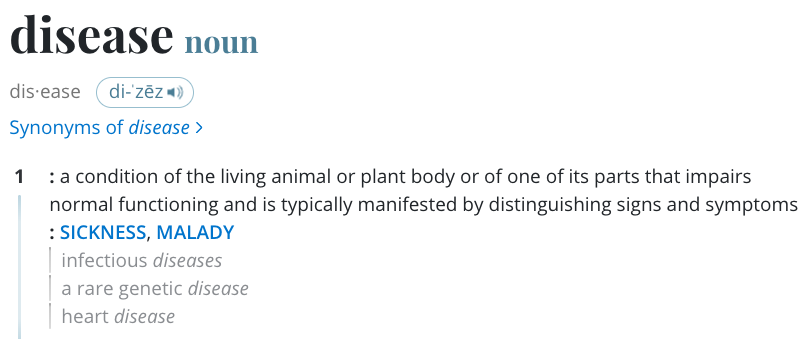
\includegraphics{images/disease_definition.png}
\end{center}
\end{block}
\end{frame}

\begin{frame}
\begin{columns}[T]
\begin{column}{0.45\textwidth}
\begin{figure}[H]

{\centering 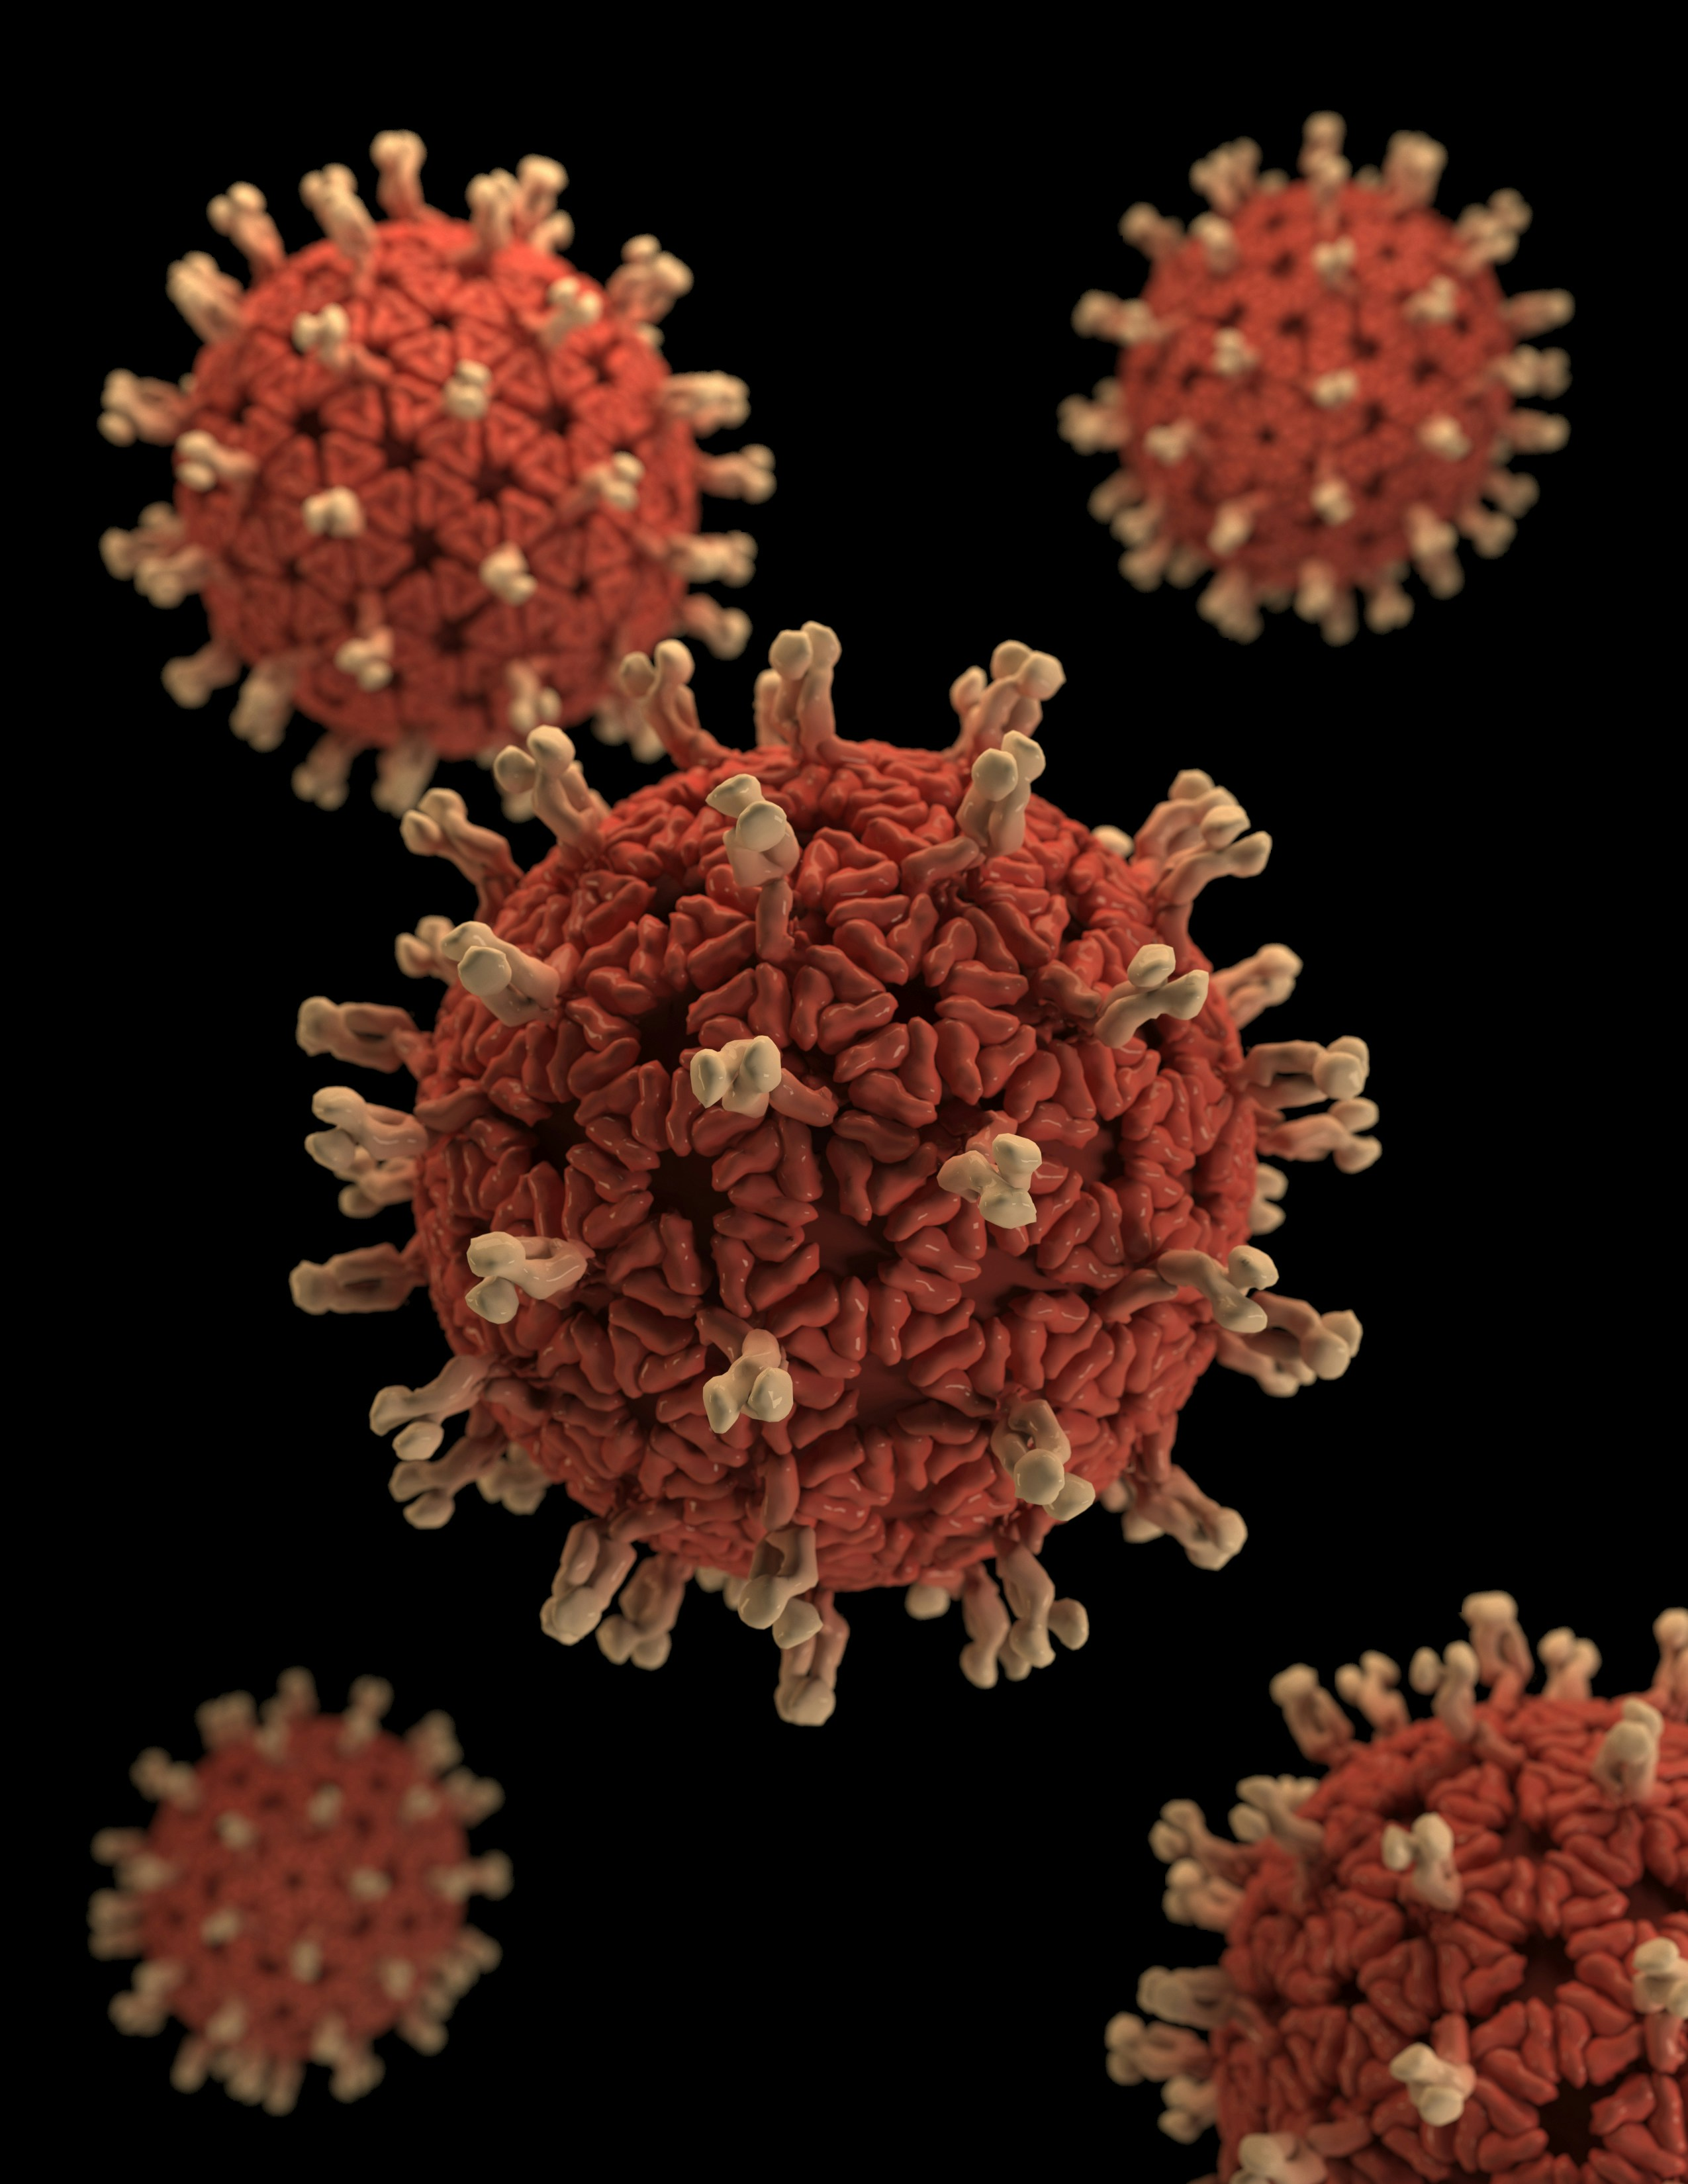
\includegraphics{images/rotavirus.jpeg}

}

\caption{A 3D graphical representation of Rotavirus virions.}

\end{figure}%
\end{column}

\begin{column}{0.55\textwidth}
Diseases can be classified according to:

\begin{itemize}
\tightlist
\item
  {Cause} (e.g., infectious, non-infectious)
\item
  {Duration} (e.g., acute, chronic)
\item
  {Mode of transmission} (direct or indirect)
\item
  {Impact} on the host (e.g., fatal, non-fatal)
\end{itemize}
\end{column}
\end{columns}
\end{frame}

\begin{frame}
Note that these classifications are not mutually exclusive. Hence, a
disease can be classified under more than one category at a time.
\end{frame}

\begin{frame}
\begin{block}{How are infectious diseases controlled?}
\phantomsection\label{sec-control-measures}
\begin{itemize}
\tightlist
\item
  In general, infectious disease control aims to reduce disease
  transmission.
\item
  The type of control used depends on the disease and its
  characteristics.
\item
  Broadly, there are two main types of control measures:

  \begin{itemize}
  \tightlist
  \item
    Pharmaceutical interventions (PIs)
  \item
    Non-pharmaceutical interventions (NPIs)
  \end{itemize}
\end{itemize}
\end{block}
\end{frame}

\begin{frame}
\begin{block}{Pharmaceutical interventions (PIs)}
\phantomsection\label{pharmaceutical-interventions-pis}
\begin{itemize}
\item
  Pharmaceutical Interventions are medical interventions that target the
  pathogen or the host.
\item
  Examples:

  \begin{itemize}
  \tightlist
  \item
    Vaccines,
  \item
    Antiviral drugs, and
  \item
    Antibiotics.
  \end{itemize}
\end{itemize}
\end{block}
\end{frame}

\begin{frame}
\begin{block}{Vaccination}
\phantomsection\label{sec-vaccination}
\begin{columns}[T]
\begin{column}{0.4\textwidth}
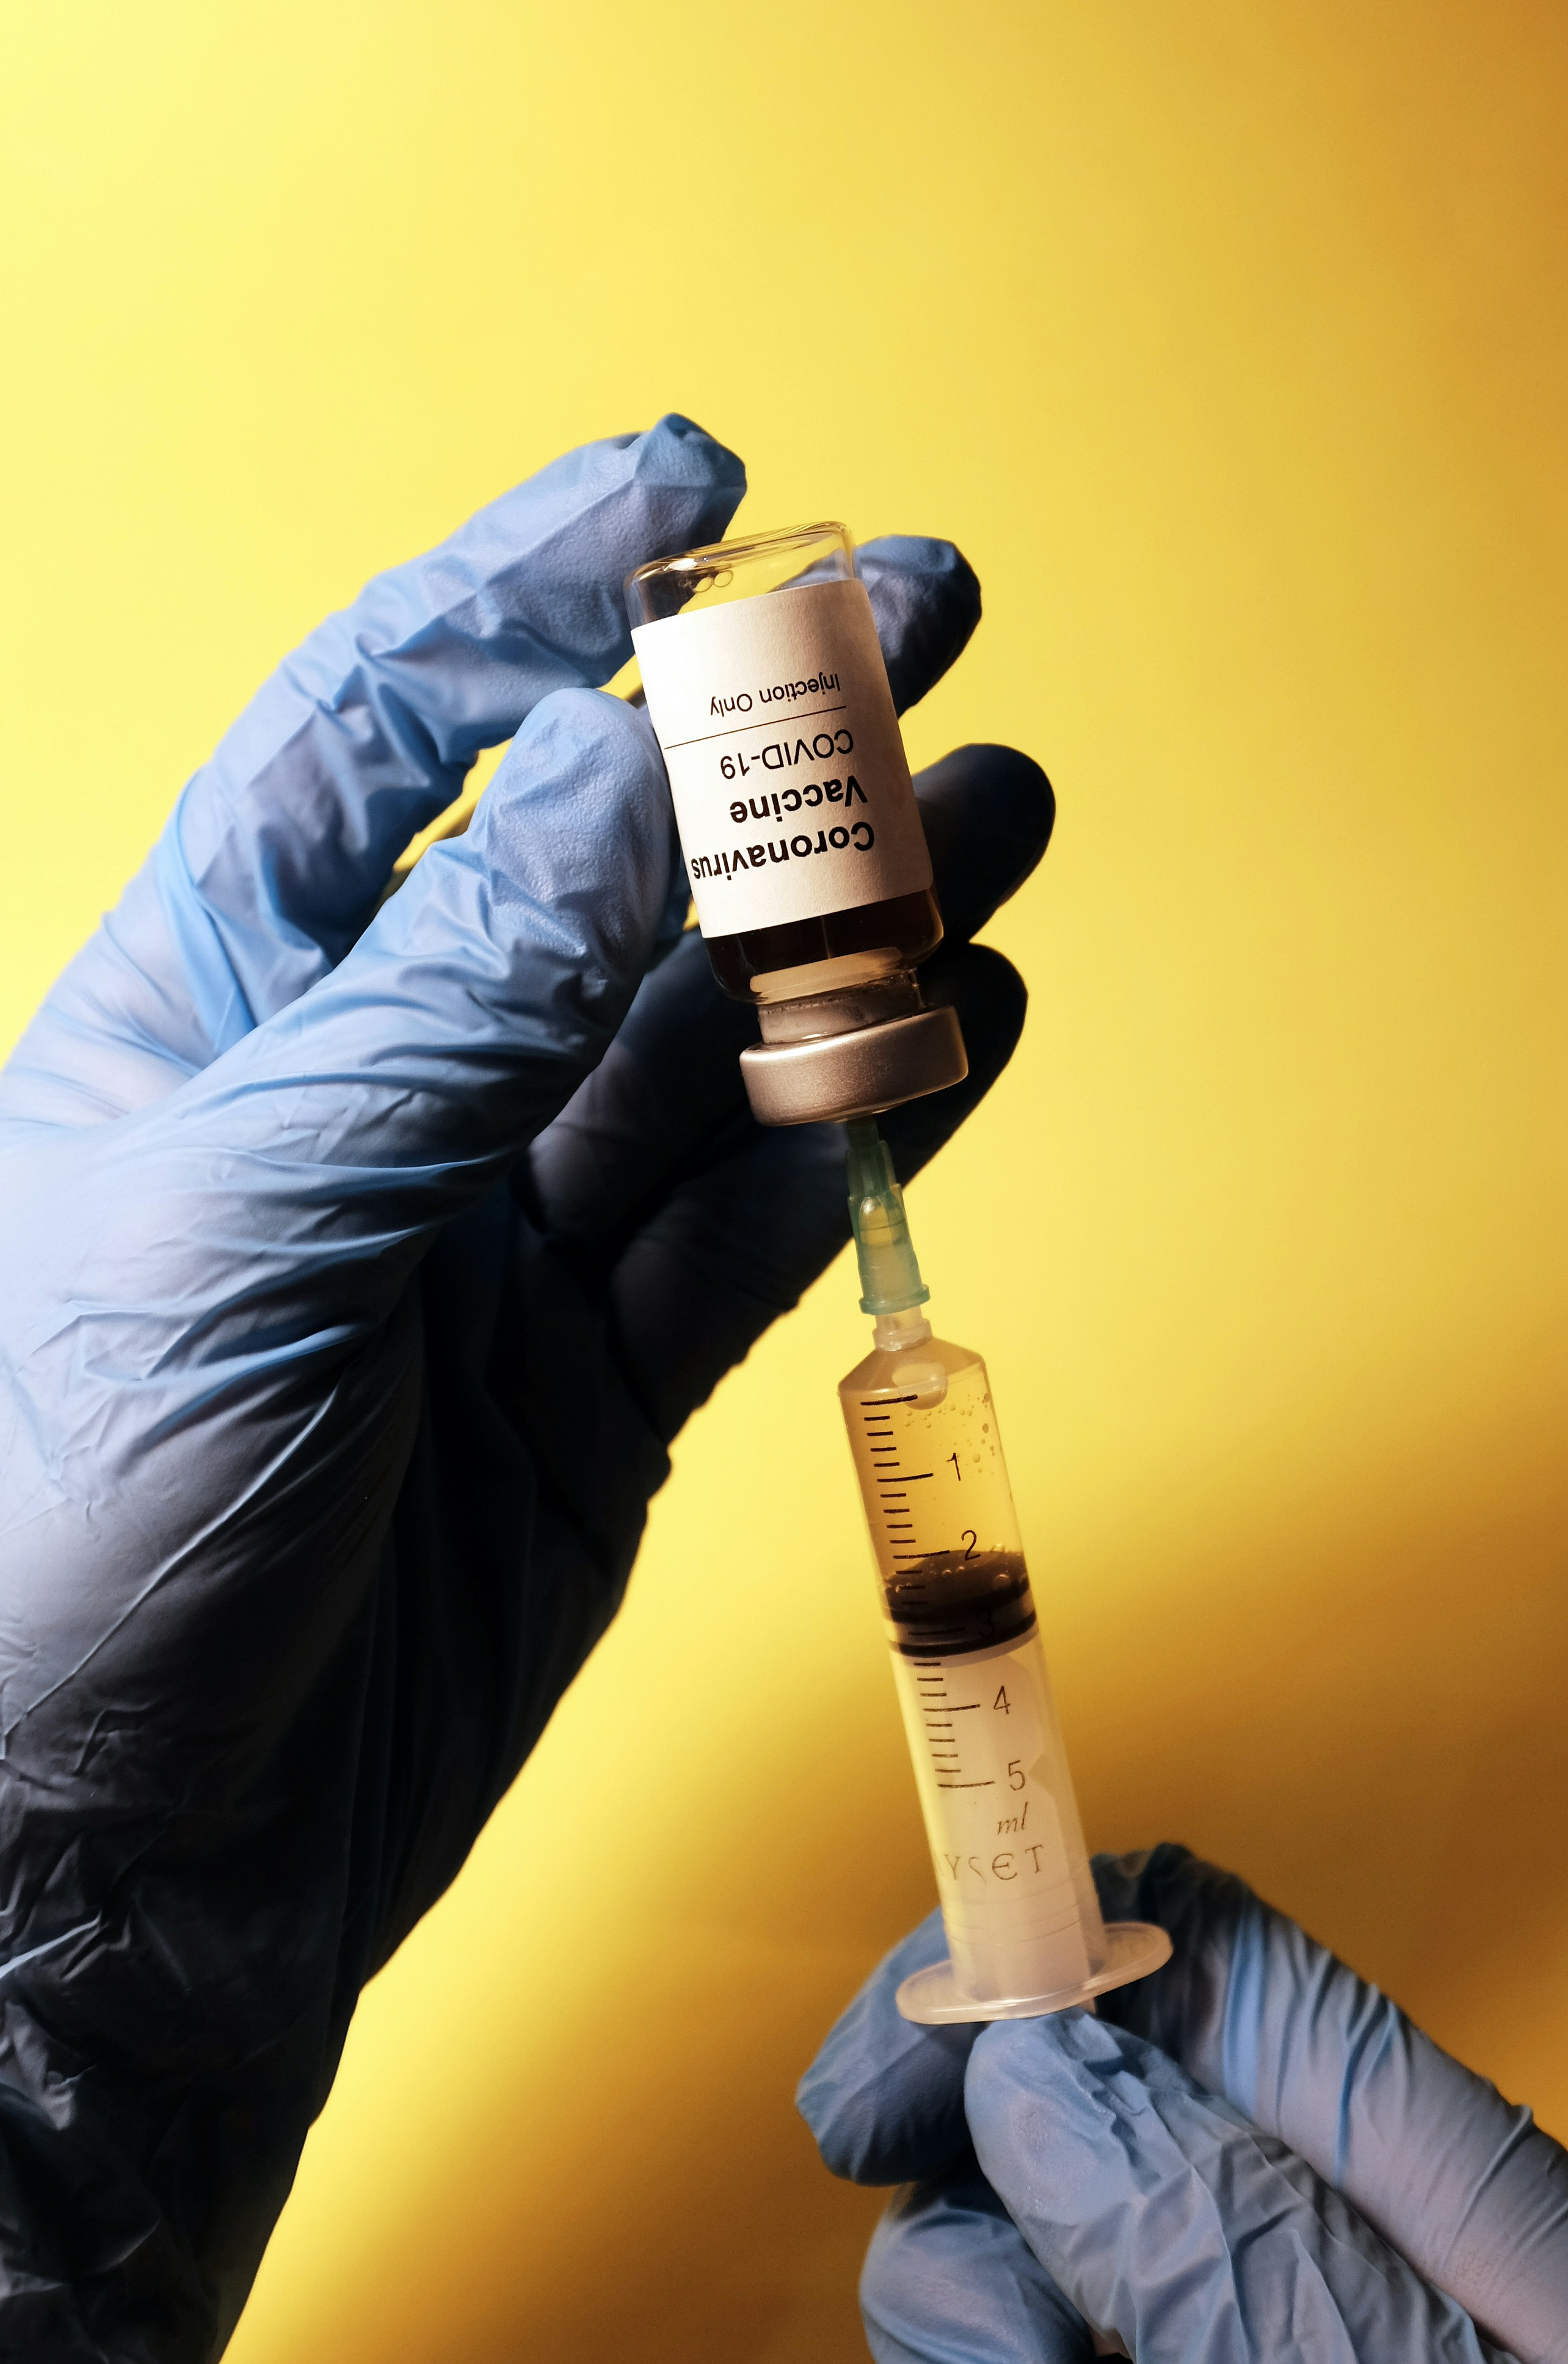
\includegraphics{images/vaccine.jpeg}
\end{column}

\begin{column}{0.6\textwidth}
\begin{itemize}
\tightlist
\item
  Activates the host's immune system to produce antibodies against the
  pathogen.
\item
  Generally applied to reduce the risk of infection and disease.
\item
  The most effective way to prevent infectious diseases.
\end{itemize}
\end{column}
\end{columns}
\end{block}
\end{frame}

\begin{frame}
\begin{block}{Challenges with vaccination}
\phantomsection\label{challenges-with-vaccination}
\begin{itemize}
\tightlist
\item
  Take time to develop for new pathogens
\item
  Never 100\% effective and limited duration of protection
\item
  Adverse side effects
\item
  Some individuals cannot be vaccinated or refuce vaccination
\item
  Some pathogens mutate rapidly (e.g., influenza virus)
\item
  Logistical challenges (e.g., cold chain requirements)
\end{itemize}
\end{block}
\end{frame}

\begin{frame}
\begin{block}{Non-pharmaceutical interventions (NPIs)}
\phantomsection\label{sec-npi}
\begin{columns}[T]
\begin{column}{0.5\textwidth}
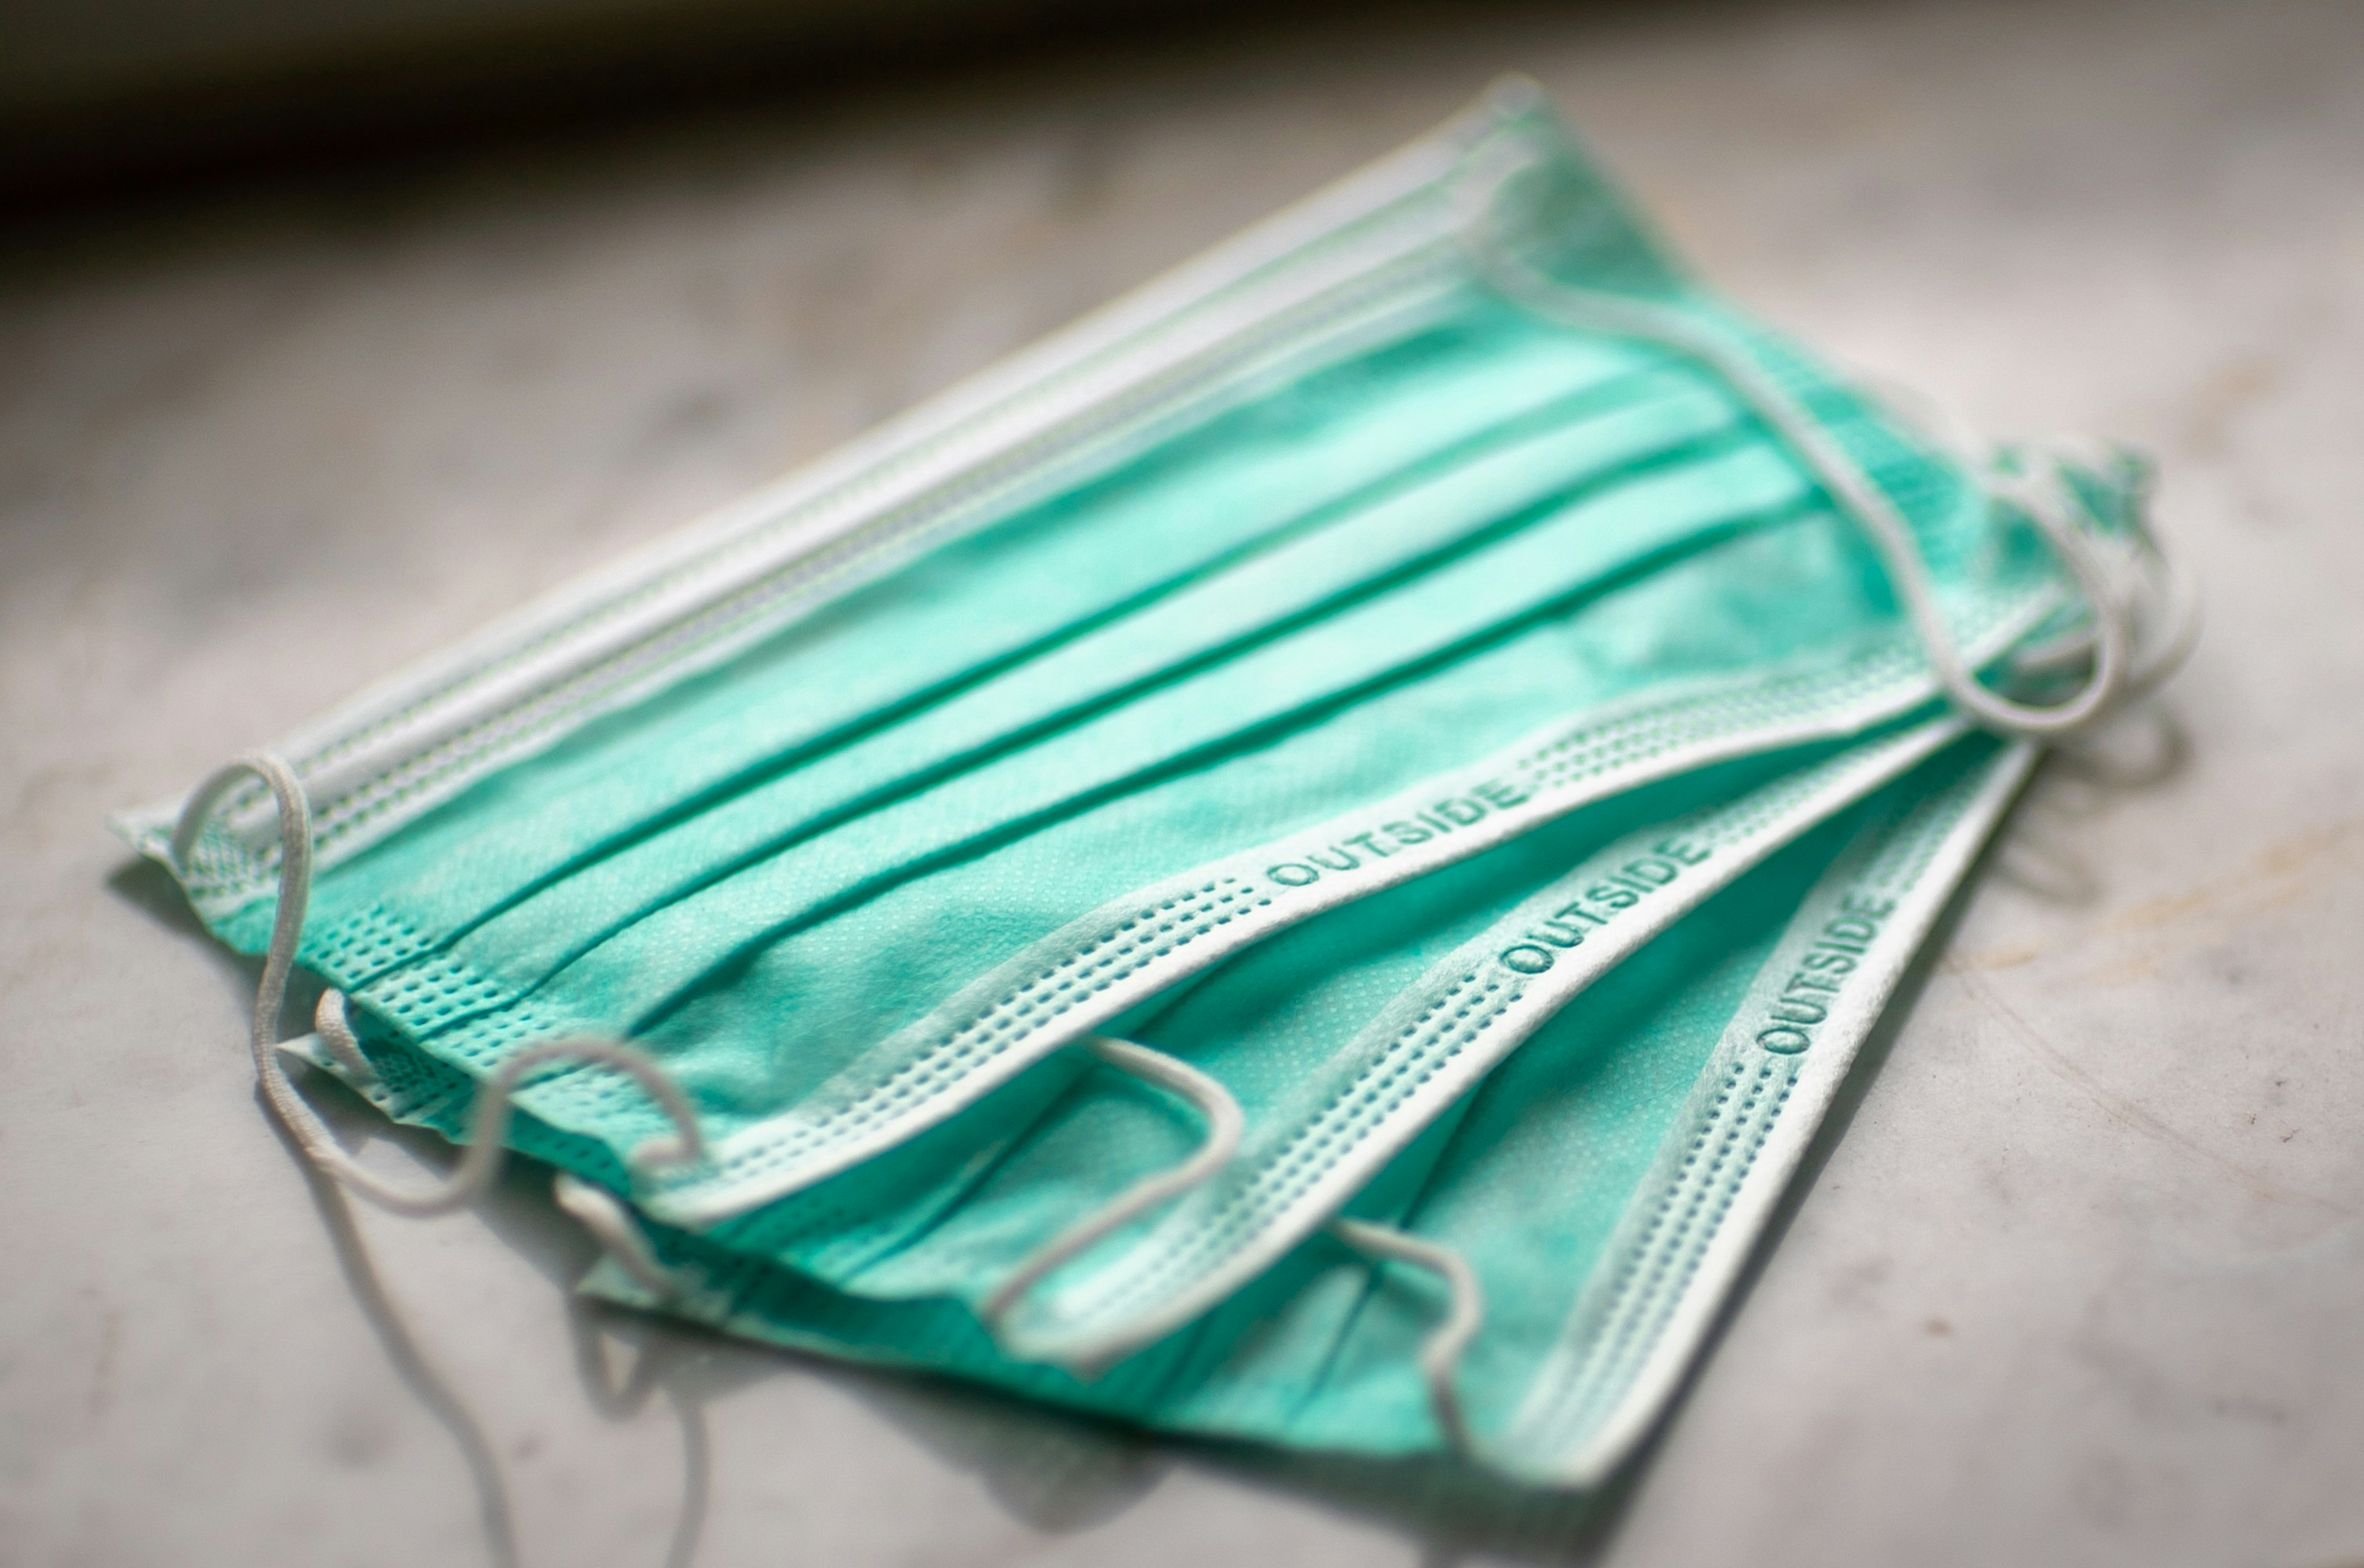
\includegraphics[width=0.7\textwidth,height=\textheight]{images/mask.jpeg}

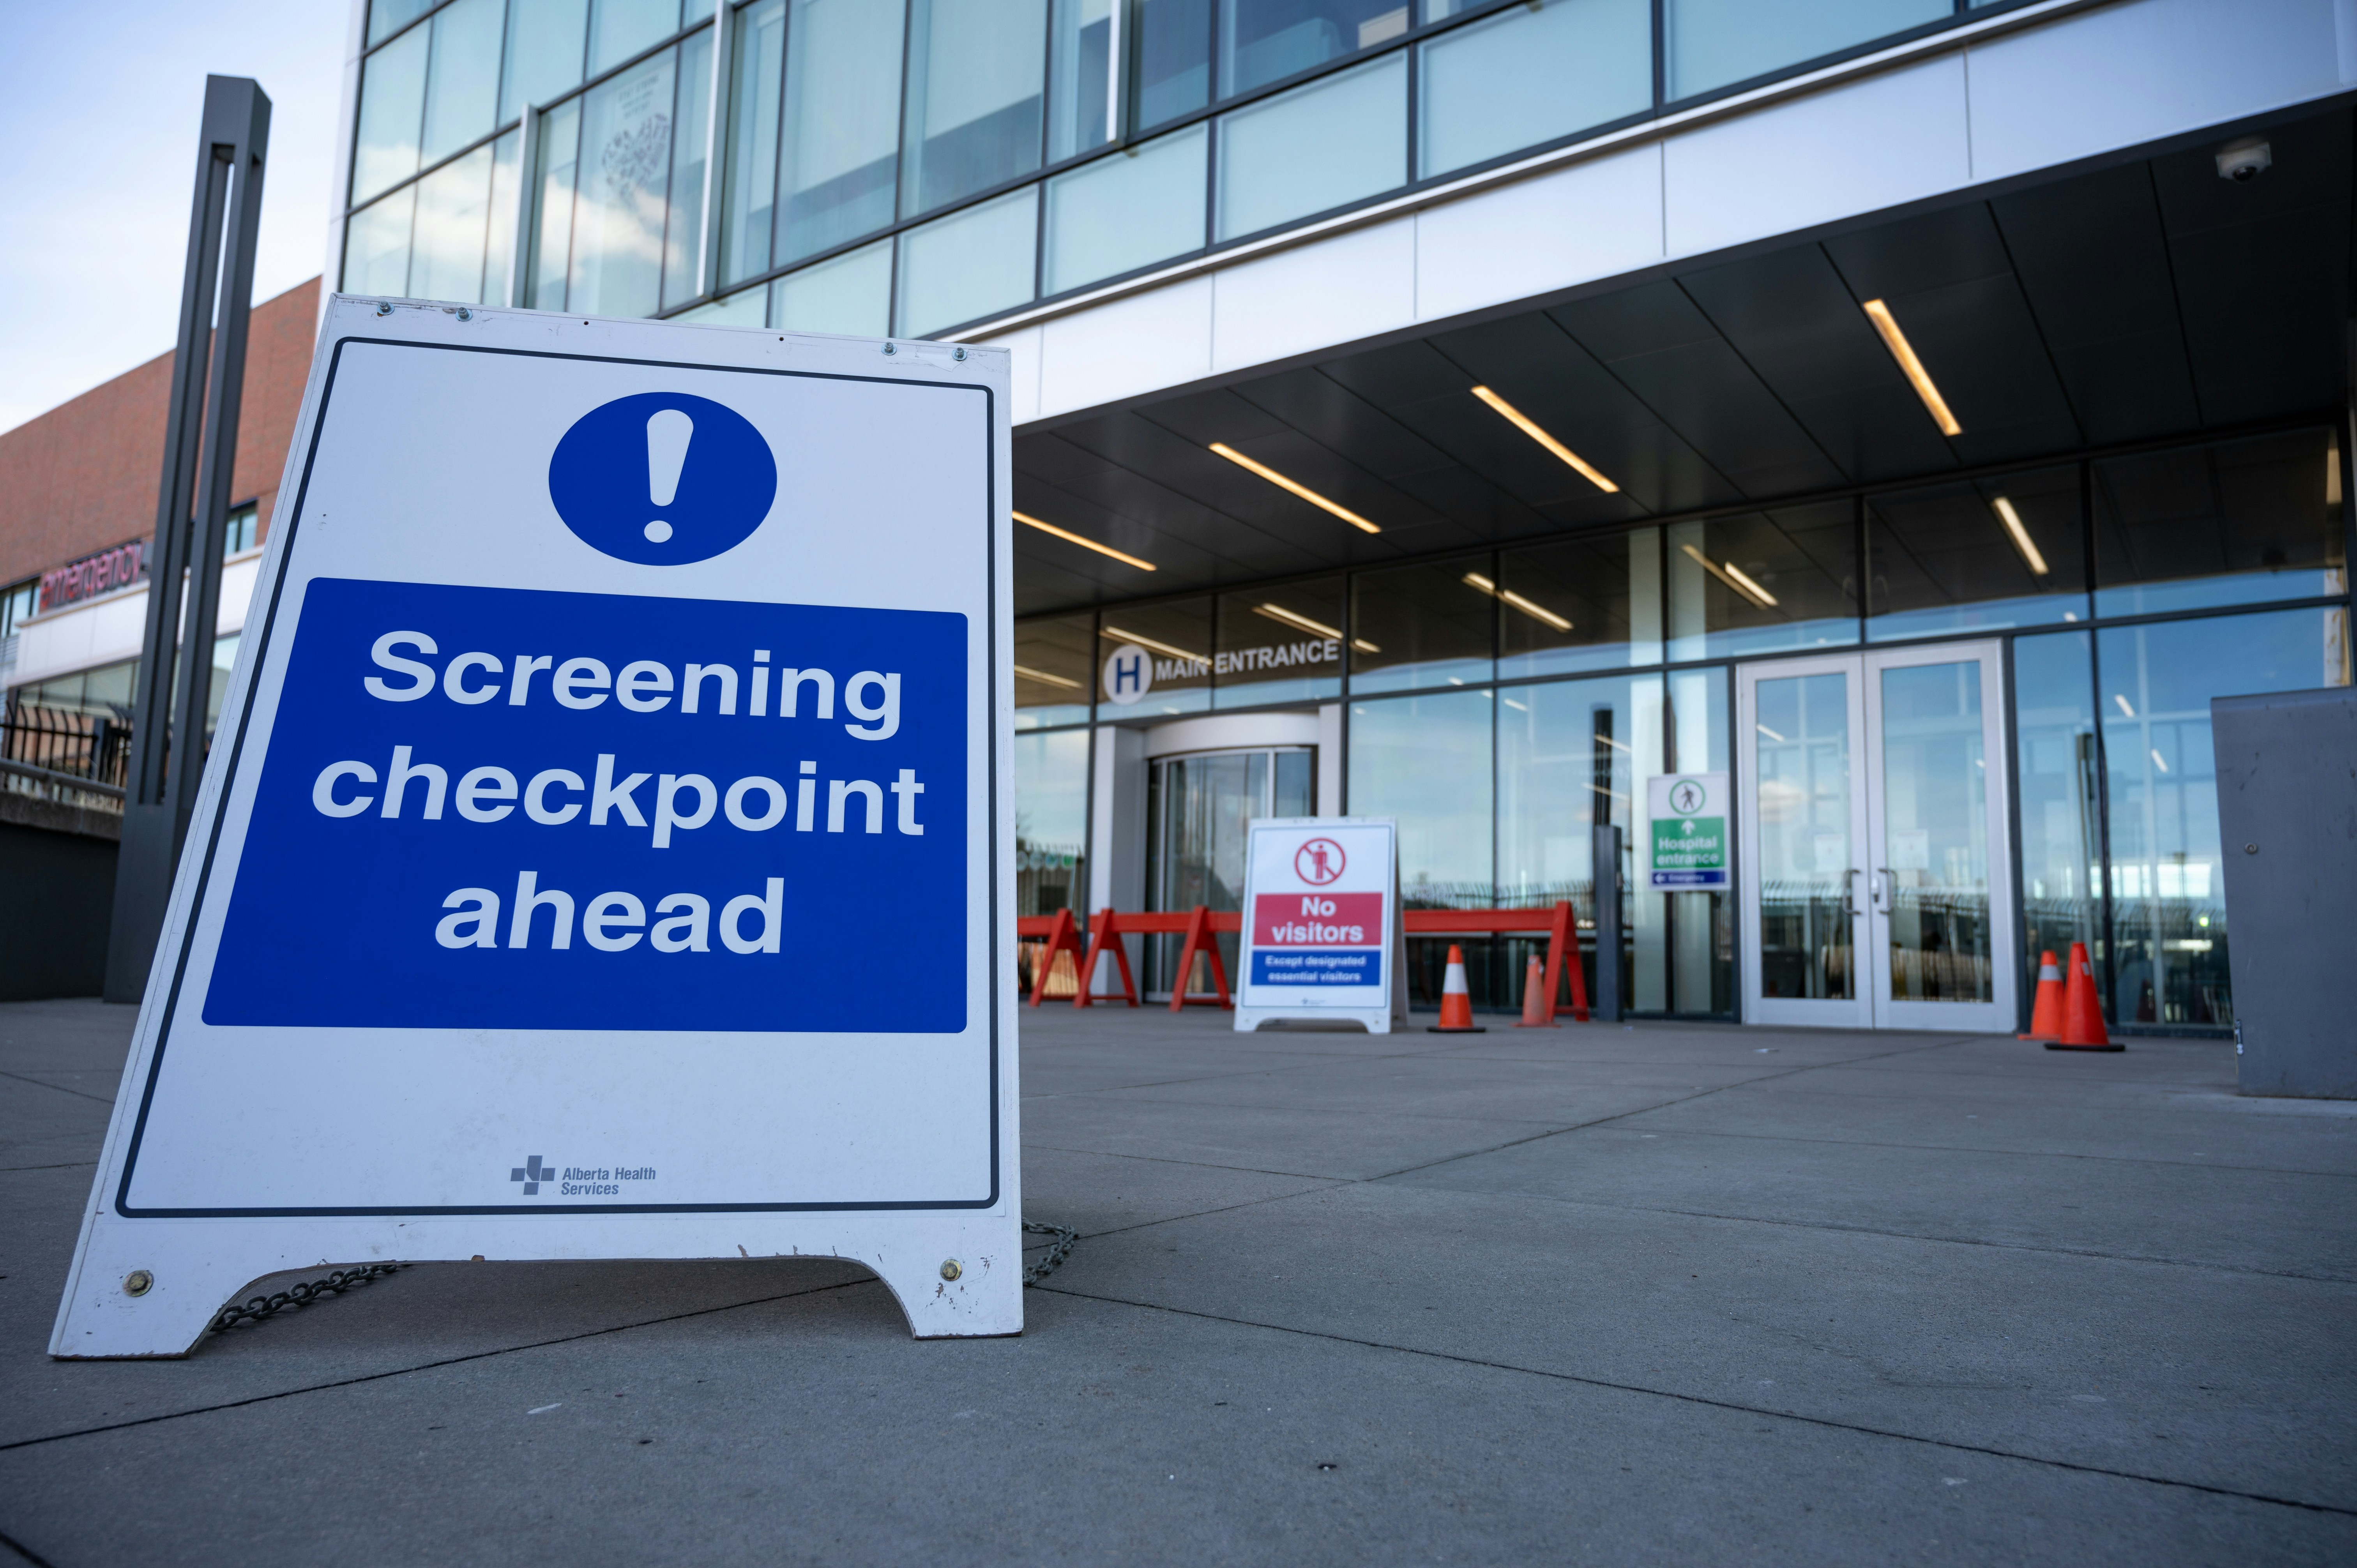
\includegraphics[width=0.7\textwidth,height=\textheight]{images/screening.jpeg}
\end{column}

\begin{column}{0.5\textwidth}
\begin{itemize}
\item
  Non-pharmaceutical interventions are measures that do not involve
  medical interventions.
\item
  Examples:

  \begin{itemize}
  \tightlist
  \item
    Quarantine,
  \item
    Physical/social distancing, and
  \item
    Mask-wearing.
  \end{itemize}
\end{itemize}
\end{column}
\end{columns}
\end{block}
\end{frame}

\begin{frame}
\begin{block}{Quarantine}
\phantomsection\label{quarantine}
\begin{itemize}
\tightlist
\item
  \emph{Isolation of individuals who may have been exposed to a
  contagious disease}.
\item
  Advantage is that it's simple and its effectiveness does not depend on
  the disease.
\item
  Disadvantages include:

  \begin{itemize}
  \tightlist
  \item
    Infringement on individual rights
  \item
    Can be difficult to enforce
  \item
    Can be costly
  \item
    Can lead to social stigma
  \end{itemize}
\end{itemize}
\end{block}
\end{frame}

\begin{frame}
\begin{block}{Contact tracing}
\phantomsection\label{contact-tracing}
\begin{itemize}
\tightlist
\item
  Contact tracing is used to identify exposed individuals, i.e.,
  individuals who might been in contact with an infected/infectious
  individual.
\item
  It involves identifying, assessing, and managing people who have been
  exposed to a contagious disease to prevent further transmission.
\item
  It is a critical component of infectious disease surveillance and is
  often used in combination with other control measures.
\end{itemize}
\end{block}
\end{frame}

\begin{frame}
\begin{tcolorbox}[enhanced jigsaw, colframe=quarto-callout-caution-color-frame, toprule=.15mm, opacitybacktitle=0.6, breakable, colback=white, leftrule=.75mm, left=2mm, opacityback=0, titlerule=0mm, bottomtitle=1mm, toptitle=1mm, title={Discussion}, bottomrule=.15mm, arc=.35mm, coltitle=black, colbacktitle=quarto-callout-caution-color!10!white, rightrule=.15mm]

\begin{itemize}
\tightlist
\item
  How can we quantify the impact of a control measure?
\end{itemize}

\end{tcolorbox}
\end{frame}

\begin{frame}{Infectious disease models}
\phantomsection\label{infectious-disease-models}
\begin{block}{What are infectious disease models?}
\phantomsection\label{what-are-infectious-disease-models}
\begin{itemize}
\tightlist
\item
  {\emph{Models}} generally refer to conceptual representations of an
  object or system.
\item
  {\emph{Mathematical models}} use mathematics to describe the system.
  For example, the famous \(E = mc^2\) is a mathematical model that
  describes the relationship between mass and energy.
\item
  {\emph{Infectious disease models}} use mathematics/statistics to
  represent dynamics/spread of infectious diseases.
\end{itemize}
\end{block}
\end{frame}

\begin{frame}
\begin{itemize}
\tightlist
\item
  Mathematical models can be used to link the biological process of
  disease transmission and the emergent dynamics of infection at the
  population level.
\item
  Models require making some assumptions and abstractions.
\end{itemize}
\end{frame}

\begin{frame}
\begin{columns}[T]
\begin{column}{0.6\textwidth}
\begin{itemize}
\tightlist
\item
  By definition, {``all models are wrong, but some are useful''}
  (\citeproc{ref-Box1979}{Box 1979}).

  \begin{itemize}
  \tightlist
  \item
    Good enough models are those that capture the {essential features}
    of the system being studied.
  \end{itemize}
\end{itemize}
\end{column}

\begin{column}{0.4\textwidth}
\begin{figure}[H]

{\centering 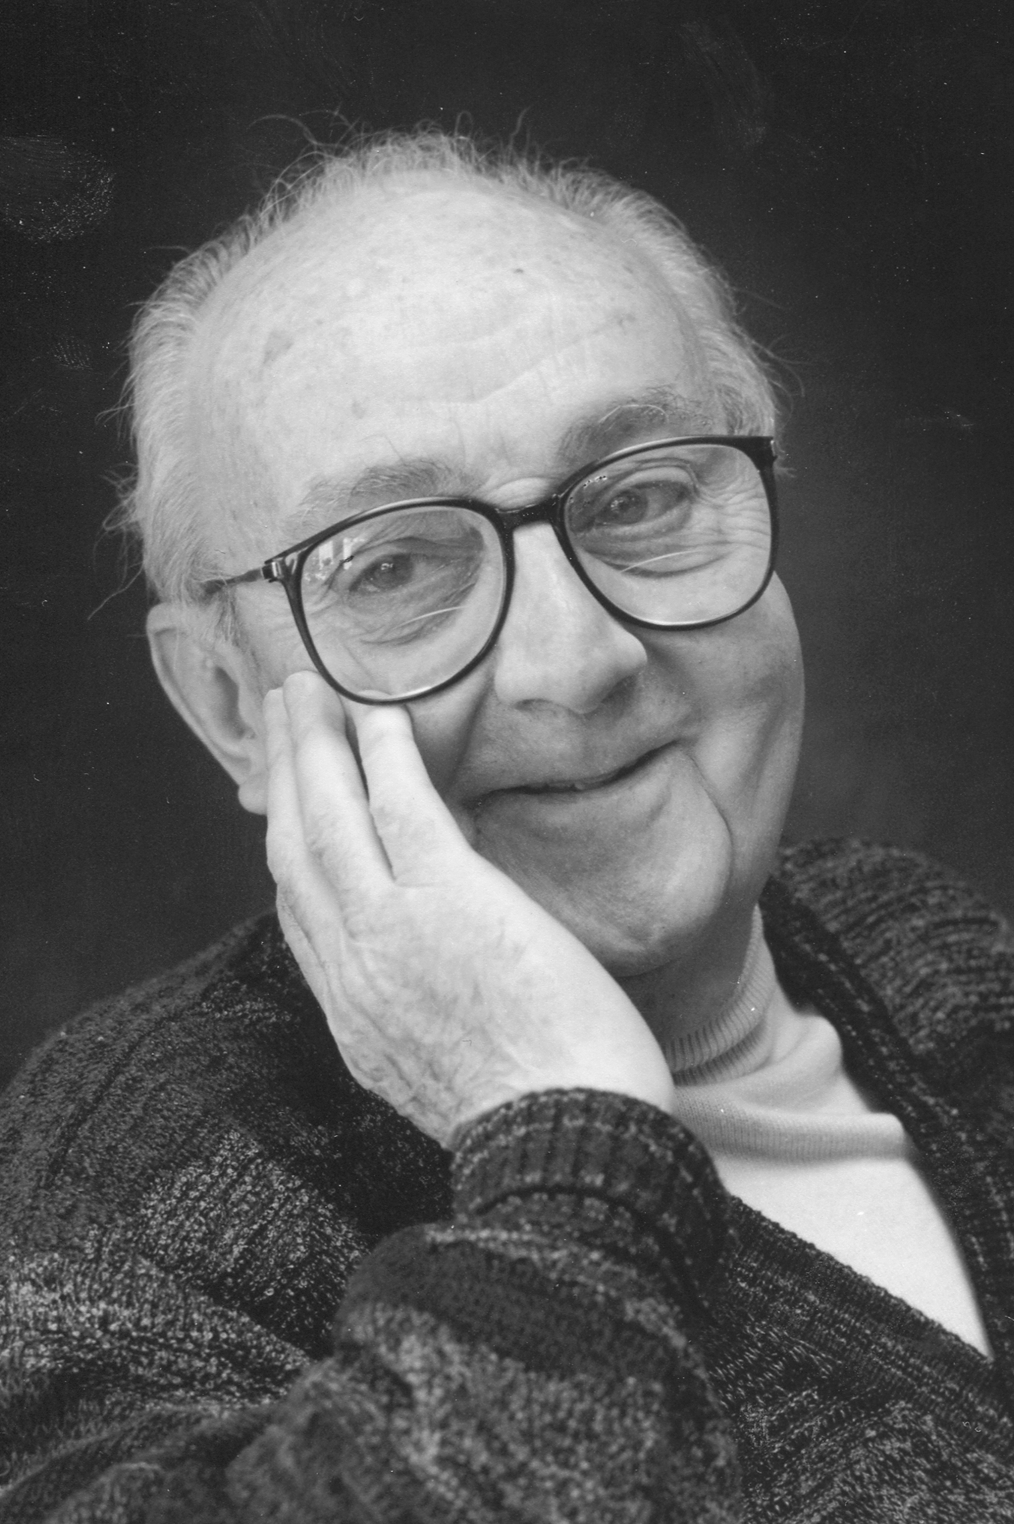
\includegraphics{images/GeorgeEPBox.jpeg}

}

\caption{George Box}

\end{figure}%
\end{column}
\end{columns}
\end{frame}

\begin{frame}
\begin{itemize}
\tightlist
\item
  What makes models ``wrong'' by definition?:

  \begin{itemize}
  \tightlist
  \item
    Simplifications of reality; not capturing all the complexities of
    the system being studied.
  \end{itemize}
\end{itemize}
\end{frame}

\begin{frame}
\begin{block}{Factors that influence model formulation/choice}
\phantomsection\label{factors-that-influence-model-formulationchoice}
\begin{itemize}
\tightlist
\item
  {Accuracy}: how well does the model to reproduce observed data and
  predict future outcomes?
\item
  {Transparency}: is it easy to understand and interpret the model and
  its outputs? (This is affected by the model's complexity)
\item
  {Flexibility}: the ability of the model to be adapted to different
  scenarios.
\end{itemize}

\note{These will be touched on in the scenario modelling lectures.}
\end{block}
\end{frame}

\begin{frame}
\begin{block}{What are models used for?}
\phantomsection\label{what-are-models-used-for}
\begin{itemize}
\tightlist
\item
  Generally, models can be used to predict and understand/explain the
  dynamics of infectious diseases.
\end{itemize}

\begin{tcolorbox}[enhanced jigsaw, colframe=quarto-callout-caution-color-frame, toprule=.15mm, opacitybacktitle=0.6, breakable, colback=white, leftrule=.75mm, left=2mm, opacityback=0, titlerule=0mm, bottomtitle=1mm, toptitle=1mm, title={Discussion}, bottomrule=.15mm, arc=.35mm, coltitle=black, colbacktitle=quarto-callout-caution-color!10!white, rightrule=.15mm]

How are these two uses impacted by accuracy, transparency, and
flexibility?

\end{tcolorbox}
\end{block}
\end{frame}

\begin{frame}
\begin{block}{Prediction of the future course}
\phantomsection\label{prediction-of-the-future-course}
\begin{columns}[T]
\begin{column}{0.4\textwidth}
\begin{itemize}
\tightlist
\item
  Must be {accurate}.
\item
  ``But the estimate proved to be off. Way, way off. Like, 65 times
  worse than what ended up happening.''
\end{itemize}
\end{column}

\begin{column}{0.6\textwidth}
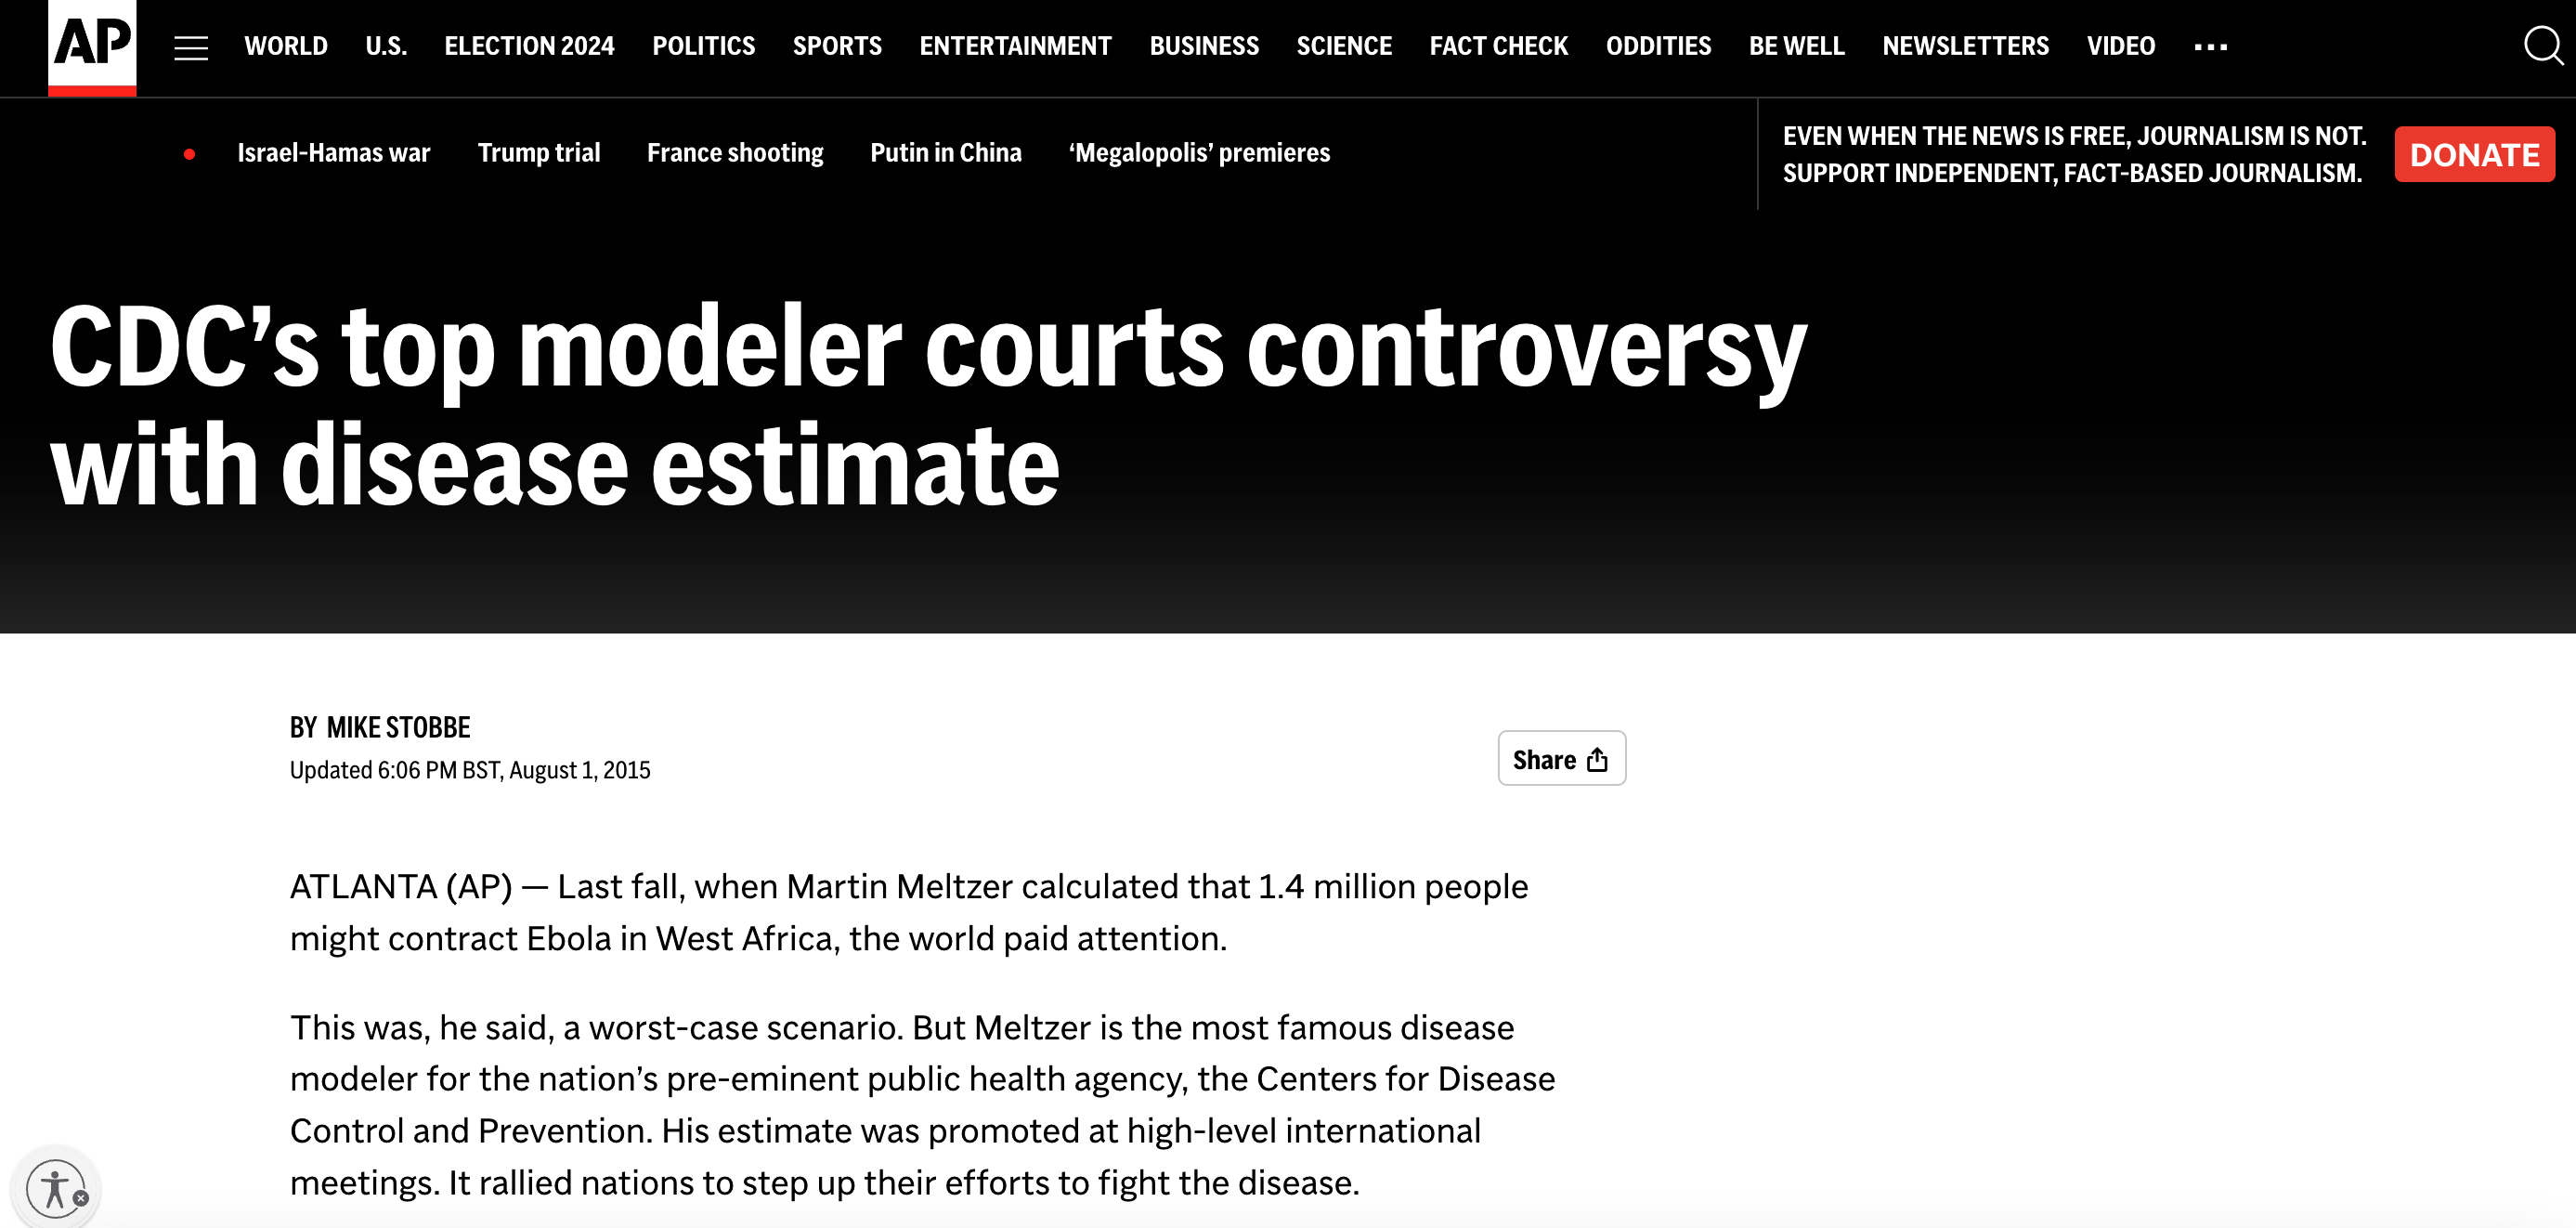
\includegraphics{images/wrong_ebola_deaths_estimate.png}
\end{column}
\end{columns}
\end{block}
\end{frame}

\begin{frame}
\begin{block}{Understanding or explaining disease dynamics}
\phantomsection\label{understanding-or-explaining-disease-dynamics}
\begin{itemize}
\tightlist
\item
  Models can be used to understand how a disease spreads and how its
  spread can be controlled.
\item
  The insights gained from models can be used to:

  \begin{itemize}
  \tightlist
  \item
    inform public health policy and interventions.
  \item
    design interventions to control the spread of the disease, for
    example, randomised controlled trials.
  \item
    collect new data.
  \item
    build predictive models.
  \end{itemize}
\end{itemize}
\end{block}
\end{frame}

\begin{frame}
\begin{block}{Limitations of infectious disease models}
\phantomsection\label{limitations-of-infectious-disease-models}
\begin{itemize}
\tightlist
\item
  Host behaviour is often difficult to predict.
\item
  The pathogen often has unknown characteristics or known
  characteristics that are difficult to model.
\item
  Data is often not available or is of poor quality.
\end{itemize}
\end{block}
\end{frame}

\begin{frame}
\begin{block}{Summary}
\phantomsection\label{summary}
\begin{itemize}
\tightlist
\item
  Models:

  \begin{itemize}
  \tightlist
  \item
    {Simplifications of reality} and do not capture all the
    {complexities} of the system being studied.
  \item
    Only as good as the {data} used to parameterize them.
  \item
    Sensitive to the {assumptions} made during their formulation.
  \item
    {Computationally expensive} and require a lot of data to run.
  \item
    {Difficult to interpret} and communicate to non-experts.
  \end{itemize}
\end{itemize}
\end{block}
\end{frame}

\begin{frame}{Introduction to compartmental models}
\phantomsection\label{introduction-to-compartmental-models}
\begin{block}{What are compartmental models?}
\phantomsection\label{what-are-compartmental-models}
\begin{itemize}
\tightlist
\item
  Compartmental models:

  \begin{itemize}
  \tightlist
  \item
    divide populations into compartments (or groups) based on the
    individual's infection status and track them through time
    (\citeproc{ref-Blackwood2018a}{Blackwood and Childs 2018}).
  \item
    are mechanistic, meaning they describe processes such the
    interaction between hosts, biological processes of pathogen, host
    immune response, and so forth.
  \end{itemize}
\end{itemize}
\end{block}
\end{frame}

\begin{frame}
Compartmental models are different from statistical models, which are
used to describe the relationship between variables.
\end{frame}

\begin{frame}
\begin{itemize}
\tightlist
\item
  Individuals in a compartment:

  \begin{itemize}
  \tightlist
  \item
    are assumed to have the same features (disease state, age, location,
    etc)
  \item
    can only be in one compartment at a time.
  \item
    move between compartments based on defined transition rates.
  \end{itemize}
\end{itemize}
\end{frame}

\begin{frame}
\begin{columns}[T]
\begin{column}{0.6\textwidth}
\begin{itemize}
\tightlist
\item
  Common compartments:

  \begin{itemize}
  \tightlist
  \item
    Susceptible (S) - hosts are not infected but can be infected
  \item
    Infected (I) - hosts are infected (and can infect others)
  \item
    Removed (R) - hosts are no longer infected and cannot be re-infected
  \end{itemize}
\end{itemize}
\end{column}

\begin{column}{0.4\textwidth}
\begin{figure}[H]

{\centering 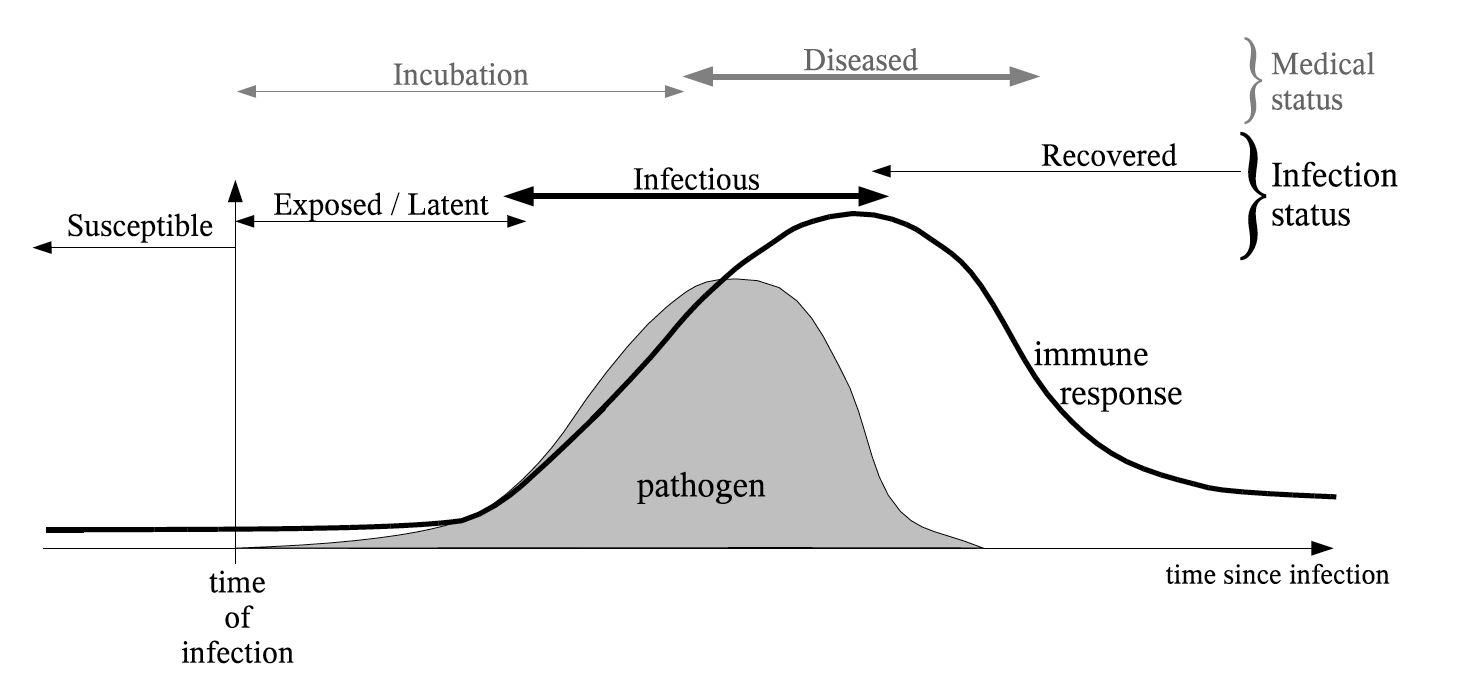
\includegraphics{images/infection_timeline.png}

}

\caption{Infection timeline illustrating how a pathogen in a host
interacts with the host's immune system (Source: Modelling Infectious
Diseases of Humans and Animals)}

\end{figure}%
\end{column}
\end{columns}
\end{frame}

\begin{frame}
\begin{itemize}
\item
  Other compartments can be added to the model to account for important
  events or processes (e.g., exposed, recovered, vaccinated, etc.)
\item
  It is, however, important to keep the model simple, less
  computationally intensive, and interpretable.
\end{itemize}
\end{frame}

\begin{frame}
\begin{itemize}
\tightlist
\item
  Compartmental models either have \emph{discrete} or \emph{continuous}
  time scales:

  \begin{itemize}
  \tightlist
  \item
    {Discrete time scales}: time is divided into discrete intervals
    (e.g., days, weeks, months).
  \item
    {Continuous time scales}: time is continuous and the model is
    described using differential equations.
  \end{itemize}
\end{itemize}
\end{frame}

\begin{frame}
\begin{itemize}
\tightlist
\item
  Compartmental models can be \emph{deterministic} or \emph{stochastic}:

  \begin{itemize}
  \tightlist
  \item
    {Deterministic} models always return the same output for the same
    input.
  \item
    {Stochastic} models account for randomness in the system and model
    output always varies. Hence, they are often run multiple times to
    get an average output.
  \end{itemize}
\end{itemize}
\end{frame}

\begin{frame}
\begin{itemize}
\tightlist
\item
  The choice of model type depends on:

  \begin{itemize}
  \tightlist
  \item
    the research {question},
  \item
    {data} availability,
  \item
    {computational resources},
  \item
    modeller {skillset}.
  \end{itemize}
\item
  In this introduction, we will focus on {deterministic compartmental
  models with continuous time scales}.
\end{itemize}
\end{frame}

\begin{frame}
\begin{itemize}
\tightlist
\item
  Now, back to the models, we are going to consider infections that
  either confer immunity after recovery or not.
\item
  The simplest compartmental models for capturing this is the SIR model.
\end{itemize}
\end{frame}

\begin{frame}
\begin{block}{The Susceptible-Infected-Recovered (SIR) model}
\phantomsection\label{the-susceptible-infected-recovered-sir-model}
\begin{center}
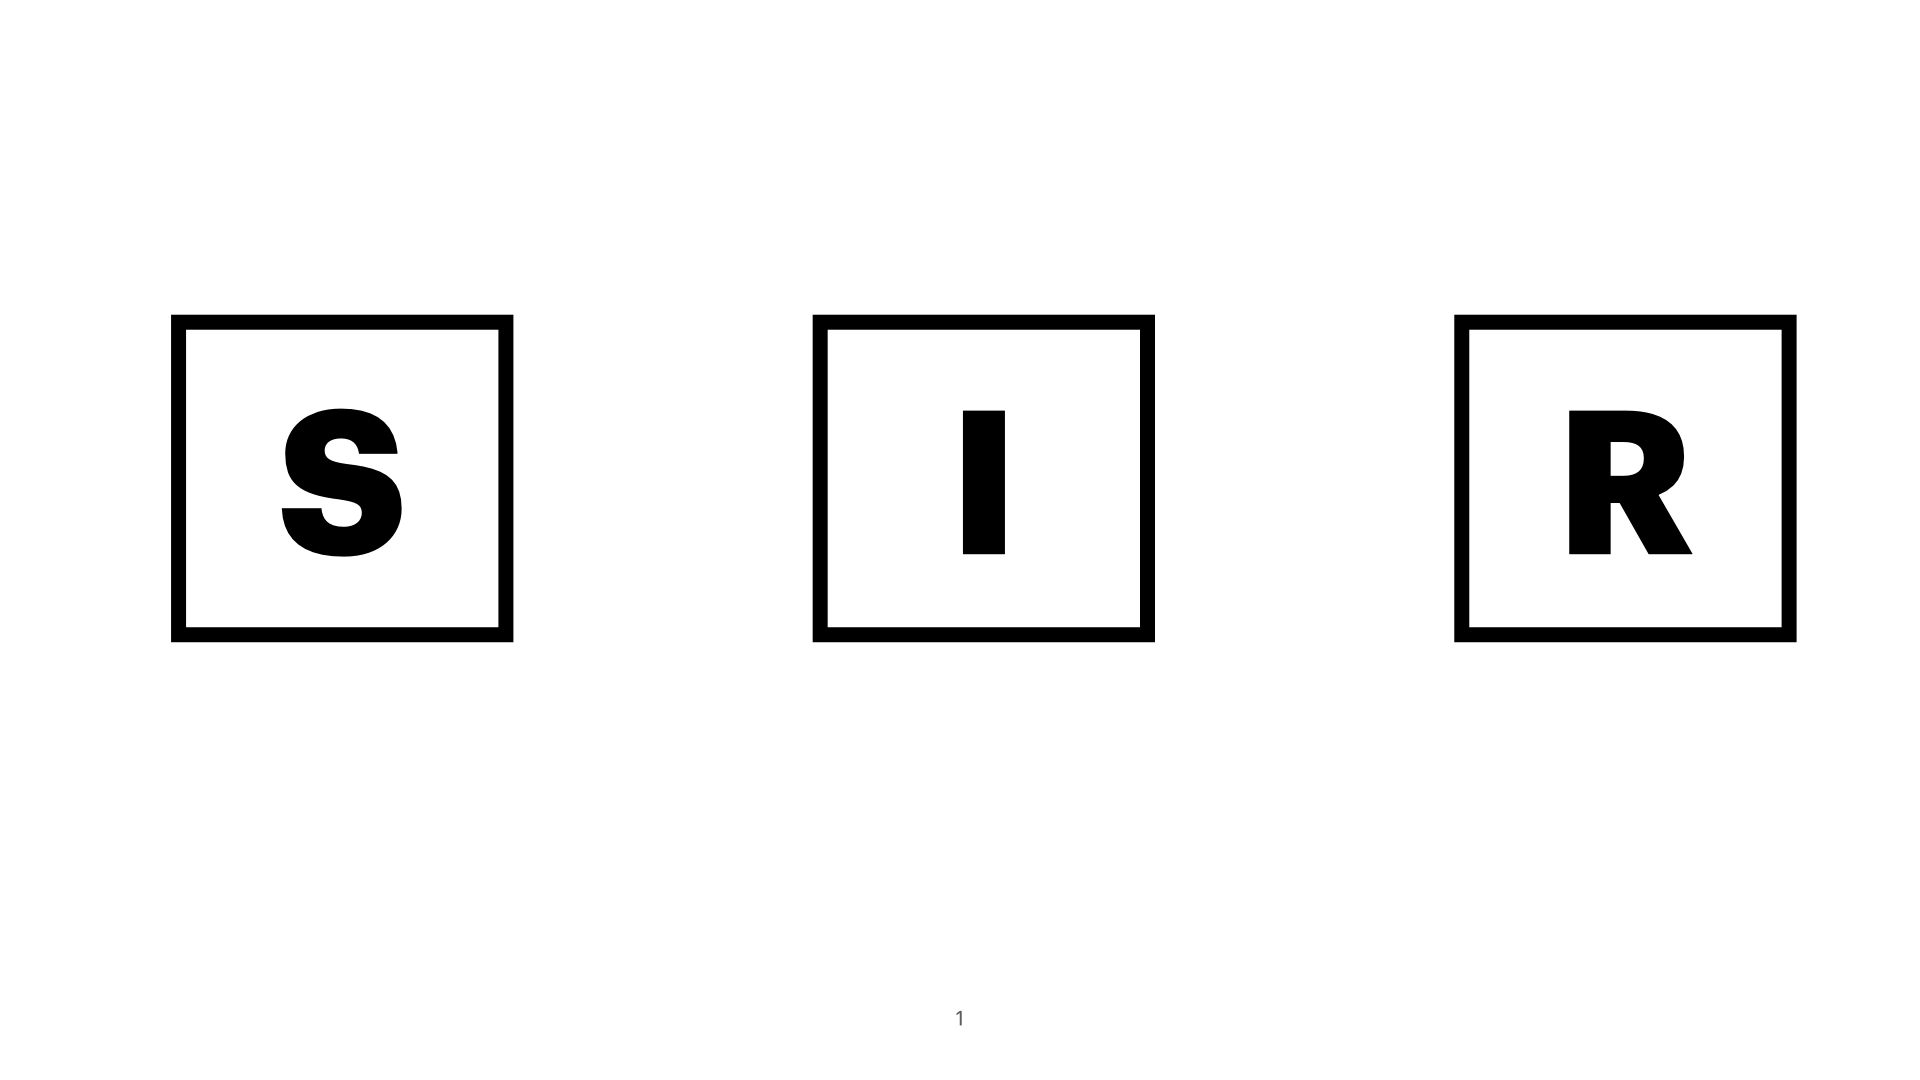
\includegraphics[width=0.4\textwidth,height=\textheight]{./images/model_diagrams/model_diagrams.001.jpeg}
\end{center}

This model groups individuals into three \emph{disease states}:

\begin{itemize}
\item
  {Susceptible (S)}: not infected but can be.
\item
  {Infected (I)}: infected \& infectious.
\item
  {Recovered/removed (R)}: recovered \& immune.
\end{itemize}
\end{block}
\end{frame}

\begin{frame}
\begin{block}{How do individuals move between compartments?}
\phantomsection\label{how-do-individuals-move-between-compartments}
\begin{block}{Process 1: Transmission}
\phantomsection\label{process-1-transmission}
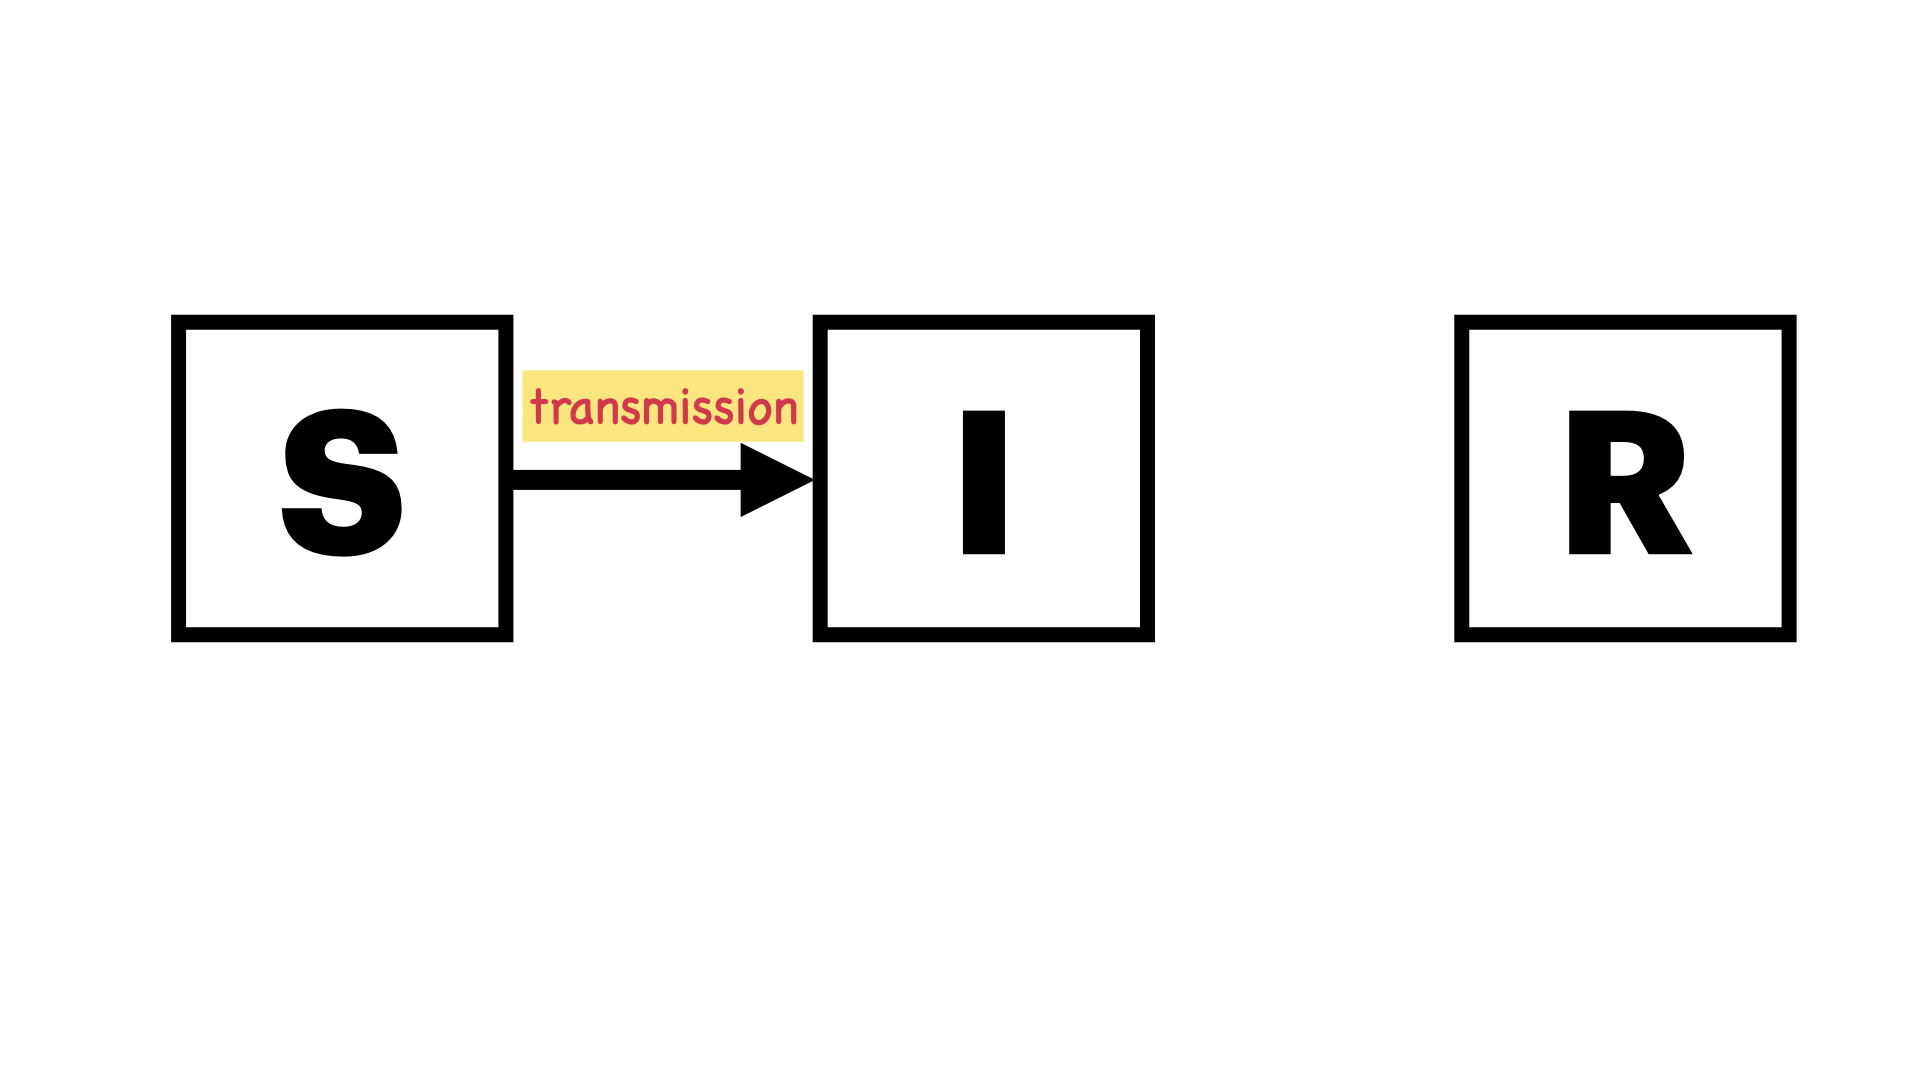
\includegraphics[width=0.7\textwidth,height=\textheight]{images/model_diagrams/model_diagrams.002.jpeg}

{What drives transmission?}
\end{block}
\end{block}
\end{frame}

\begin{frame}
\begin{itemize}
\tightlist
\item
  Transmission is driven by several factors, including:

  \begin{itemize}
  \tightlist
  \item
    Disease prevalence, {\(I\)}, i.e., number of infected individuals at
    the time.
  \item
    The number of contacts, {\(C\)}, susceptible individuals have with
    infected individual.
  \item
    The probability, {\(p\)}, a susceptible individual will become
    infected when they contact an infected individual.
  \end{itemize}
\end{itemize}
\end{frame}

\begin{frame}
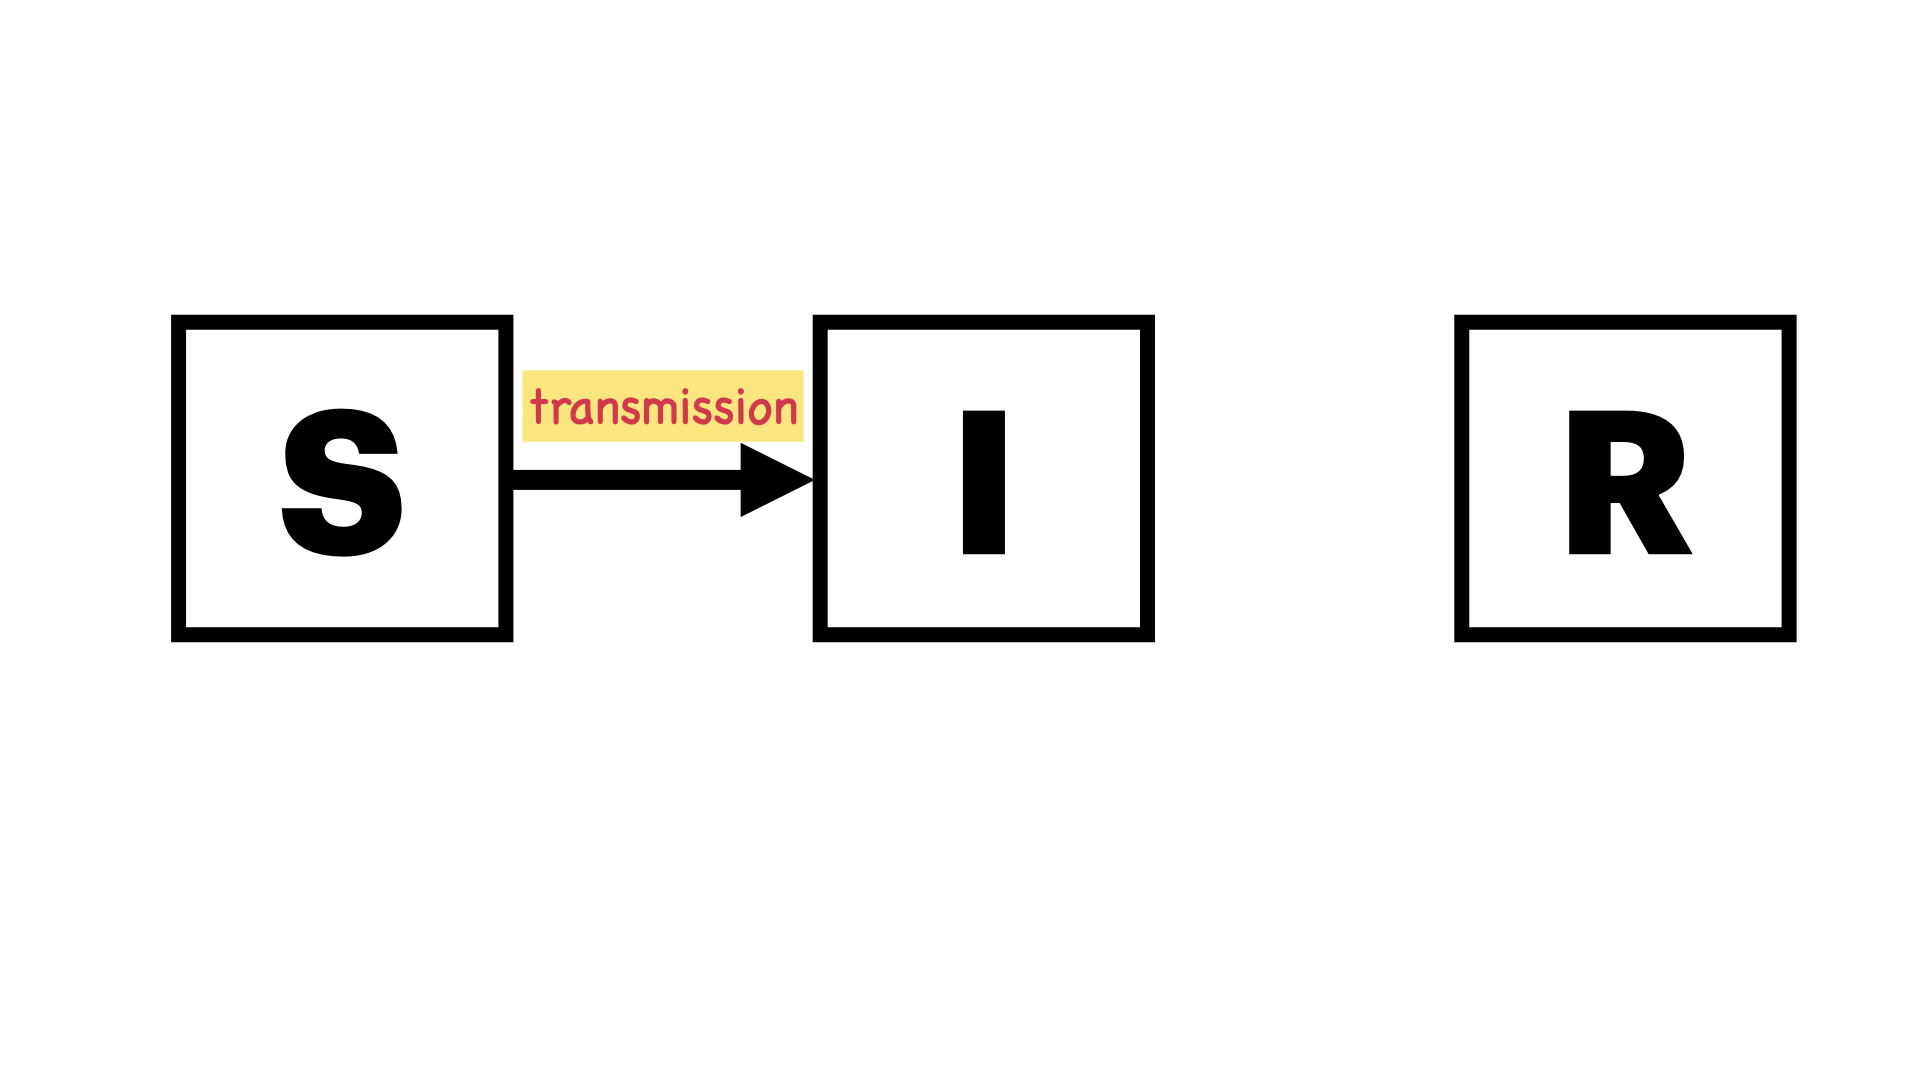
\includegraphics[width=0.7\textwidth,height=\textheight]{images/model_diagrams/model_diagrams.002.jpeg}

The transmission term is often defined through the {force of infection
(FOI), \(\lambda\)}.
\end{frame}

\begin{frame}
\begin{block}{A tour of the force of infection (FOI)}
\phantomsection\label{a-tour-of-the-force-of-infection-foi}
\begin{itemize}
\tightlist
\item
  FOI, \(\lambda\), is the {per capita rate} at which susceptible
  individuals become infected.
\end{itemize}

\begin{tcolorbox}[enhanced jigsaw, colframe=quarto-callout-note-color-frame, toprule=.15mm, opacitybacktitle=0.6, breakable, colback=white, leftrule=.75mm, left=2mm, opacityback=0, titlerule=0mm, bottomtitle=1mm, toptitle=1mm, title={Note}, bottomrule=.15mm, arc=.35mm, coltitle=black, colbacktitle=quarto-callout-note-color!10!white, rightrule=.15mm]

``Per capita'' means the rate of an event occurring per individual in
the population per unit of time.

\end{tcolorbox}

\begin{itemize}
\tightlist
\item
  Given the rate per individual per time, FOI, the rate at which new
  infecteds are generated is given by {\(\lambda \times S\)}, where
  \(S\) is the number of susceptible individuals.
\end{itemize}
\end{block}
\end{frame}

\begin{frame}
\begin{itemize}
\tightlist
\item
  The force of infection is made up of the probabilities/rates that:

  \begin{itemize}
  \tightlist
  \item
    contacts happen, {\(c\)},
  \item
    a given contact is with an infected individual, {\(p\)}, and
  \item
    a contact results in successful transmission, {\(v\)}.
  \end{itemize}
\end{itemize}
\end{frame}

\begin{frame}
\begin{itemize}
\tightlist
\item
  The FOI can be formulated in two ways, depending on how the contact
  rate is expected to change with the population size:

  \begin{itemize}
  \tightlist
  \item
    Frequency-dependent/mass action transmission
  \item
    Density-dependent transmission
  \end{itemize}
\end{itemize}
\end{frame}

\begin{frame}
\begin{block}{Frequency-dependent/mass action transmission}
\phantomsection\label{frequency-dependentmass-action-transmission}
The rate of contact between individuals is constant irrespective of the
population density, {\(\dfrac{N}{A}\)}, where {\(N\)} is the population
size and {\(A\)} is the area occupied by the population.
\end{block}
\end{frame}

\begin{frame}
\begin{itemize}
\item
  Recall that transmission also depends on the probability of contact
  with an infected host, {\(p\)}, which is assumed to be
  {\(\dfrac{I}{N}\)}.
\item
  Hence, the frequency-dependent mass action is given by
  {\(\lambda = \beta \times \dfrac{I}{N}\)}, where {\(\beta\)} is the
  transmission rate.
\end{itemize}
\end{frame}

\begin{frame}
\begin{tcolorbox}[enhanced jigsaw, colframe=quarto-callout-caution-color-frame, toprule=.15mm, opacitybacktitle=0.6, breakable, colback=white, leftrule=.75mm, left=2mm, opacityback=0, titlerule=0mm, bottomtitle=1mm, toptitle=1mm, title={Question}, bottomrule=.15mm, arc=.35mm, coltitle=black, colbacktitle=quarto-callout-caution-color!10!white, rightrule=.15mm]

Why does the frequency-dependent transmission contain {\(\dfrac{1}{N}\)}
if it does not depend on the population density?

\end{tcolorbox}
\end{frame}

\begin{frame}
\begin{itemize}
\tightlist
\item
  Assume that the rate of new infections is given by
  {\(\dfrac{dI}{dt} = S \times c \times p \times v\)} where {\(S\)} is
  the number of susceptible hosts, {\(c\)} is the contact rate, and
  {\(p\)} is the probability of contact with an infected host, and
  {\(v\)} is the probability of transmission per contact.
\end{itemize}
\end{frame}

\begin{frame}
\begin{itemize}
\item
  {\(p\)} is usually assumed to be the disease prevalence,
  {\(\dfrac{I}{N}\)}.
\item
  Hence, the rate of new infections,
  {\(\dfrac{dI}{dt} = S \times c \times \dfrac{I}{N}  \times v\)}.
\end{itemize}
\end{frame}

\begin{frame}
\begin{itemize}
\tightlist
\item
  In frequency dependent transmission, the contact rate {\(c\)} is also
  assumed to be constant, say {\(c = \eta\)} irrespective of population
  density, {\(\dfrac{N}{A}\)}, where {\(N\)} is the population size and
  {\(A\)} is the area occupied by the population.
\item
  Hence,
  {\(\dfrac{dI}{dt} = S \times \eta \times v \times \dfrac{I}{N}\)}
\item
  Therefore, {\(\dfrac{dI}{dt} = \beta S \times \dfrac{I}{N}\)}, where
  {\(\beta = \eta \times v\)}, and
  {\(\lambda = \beta \times \dfrac{I}{N}\)}.
\end{itemize}
\end{frame}

\begin{frame}
\begin{itemize}
\tightlist
\item
  {\emph{Frequency-dependent/mass action transmission}} is often used to
  model sexually-transmitted diseases and diseases with heterogeneity in
  contact rates.
\item
  Sexual transmission in this case does not depend on how many infected
  individuals are in the population.
\end{itemize}
\end{frame}

\begin{frame}
\begin{block}{Density dependent transmission}
\phantomsection\label{density-dependent-transmission}
\begin{itemize}
\item
  The rate of contact between individuals depends on the population
  density, {\(\dfrac{N}{A}\)}.
\item
  Transmission also depends on {\(p\)} - the probability that a given
  contact is with an infected individual, often taken to be
  {\(\dfrac{I}{N}\)}.
\end{itemize}
\end{block}
\end{frame}

\begin{frame}
\begin{itemize}
\item
  The density-dependent transmission is therefore given as
  {\(\lambda = \beta \times \dfrac{I}{A}\)}.
\item
  Here, because transmission increases with the density of infected
  individuals, it is called density-dependent transmission.
\end{itemize}

\begin{tcolorbox}[enhanced jigsaw, colframe=quarto-callout-note-color-frame, toprule=.15mm, opacitybacktitle=0.6, breakable, colback=white, leftrule=.75mm, left=2mm, opacityback=0, titlerule=0mm, bottomtitle=1mm, toptitle=1mm, title={Note}, bottomrule=.15mm, arc=.35mm, coltitle=black, colbacktitle=quarto-callout-note-color!10!white, rightrule=.15mm]

\begin{itemize}
\item
  Notice that
  {\(\lambda = \beta \times \dfrac{I}{N} \times \dfrac{N}{A}\)} and the
  \(N's\) cancel out.
\item
  {\(A\)} is often ignored.
\end{itemize}

\end{tcolorbox}
\end{frame}

\begin{frame}
\begin{itemize}
\tightlist
\item
  {\emph{Density dependent transmission}} can be used to model airborne
  and directly transmitted diseases, for example, measles.
\end{itemize}
\end{frame}

\begin{frame}
\begin{tcolorbox}[enhanced jigsaw, colframe=quarto-callout-caution-color-frame, toprule=.15mm, opacitybacktitle=0.6, breakable, colback=white, leftrule=.75mm, left=2mm, opacityback=0, titlerule=0mm, bottomtitle=1mm, toptitle=1mm, title={Density-dependent vs frequency dependent transmission}, bottomrule=.15mm, arc=.35mm, coltitle=black, colbacktitle=quarto-callout-caution-color!10!white, rightrule=.15mm]

This is one of the most confused and debated concepts in disease
modelling. Several studies have attempted to clarify it, including the
brilliant work by
(\citeproc{ref-begon2002clarification}{\textbf{begon2002clarification?}}).
Most of the clarifications provided here are based on this paper.

\end{tcolorbox}

\begin{itemize}
\tightlist
\item
  We will only use the {density-dependent} formulation in this course.
\end{itemize}
\end{frame}

\begin{frame}
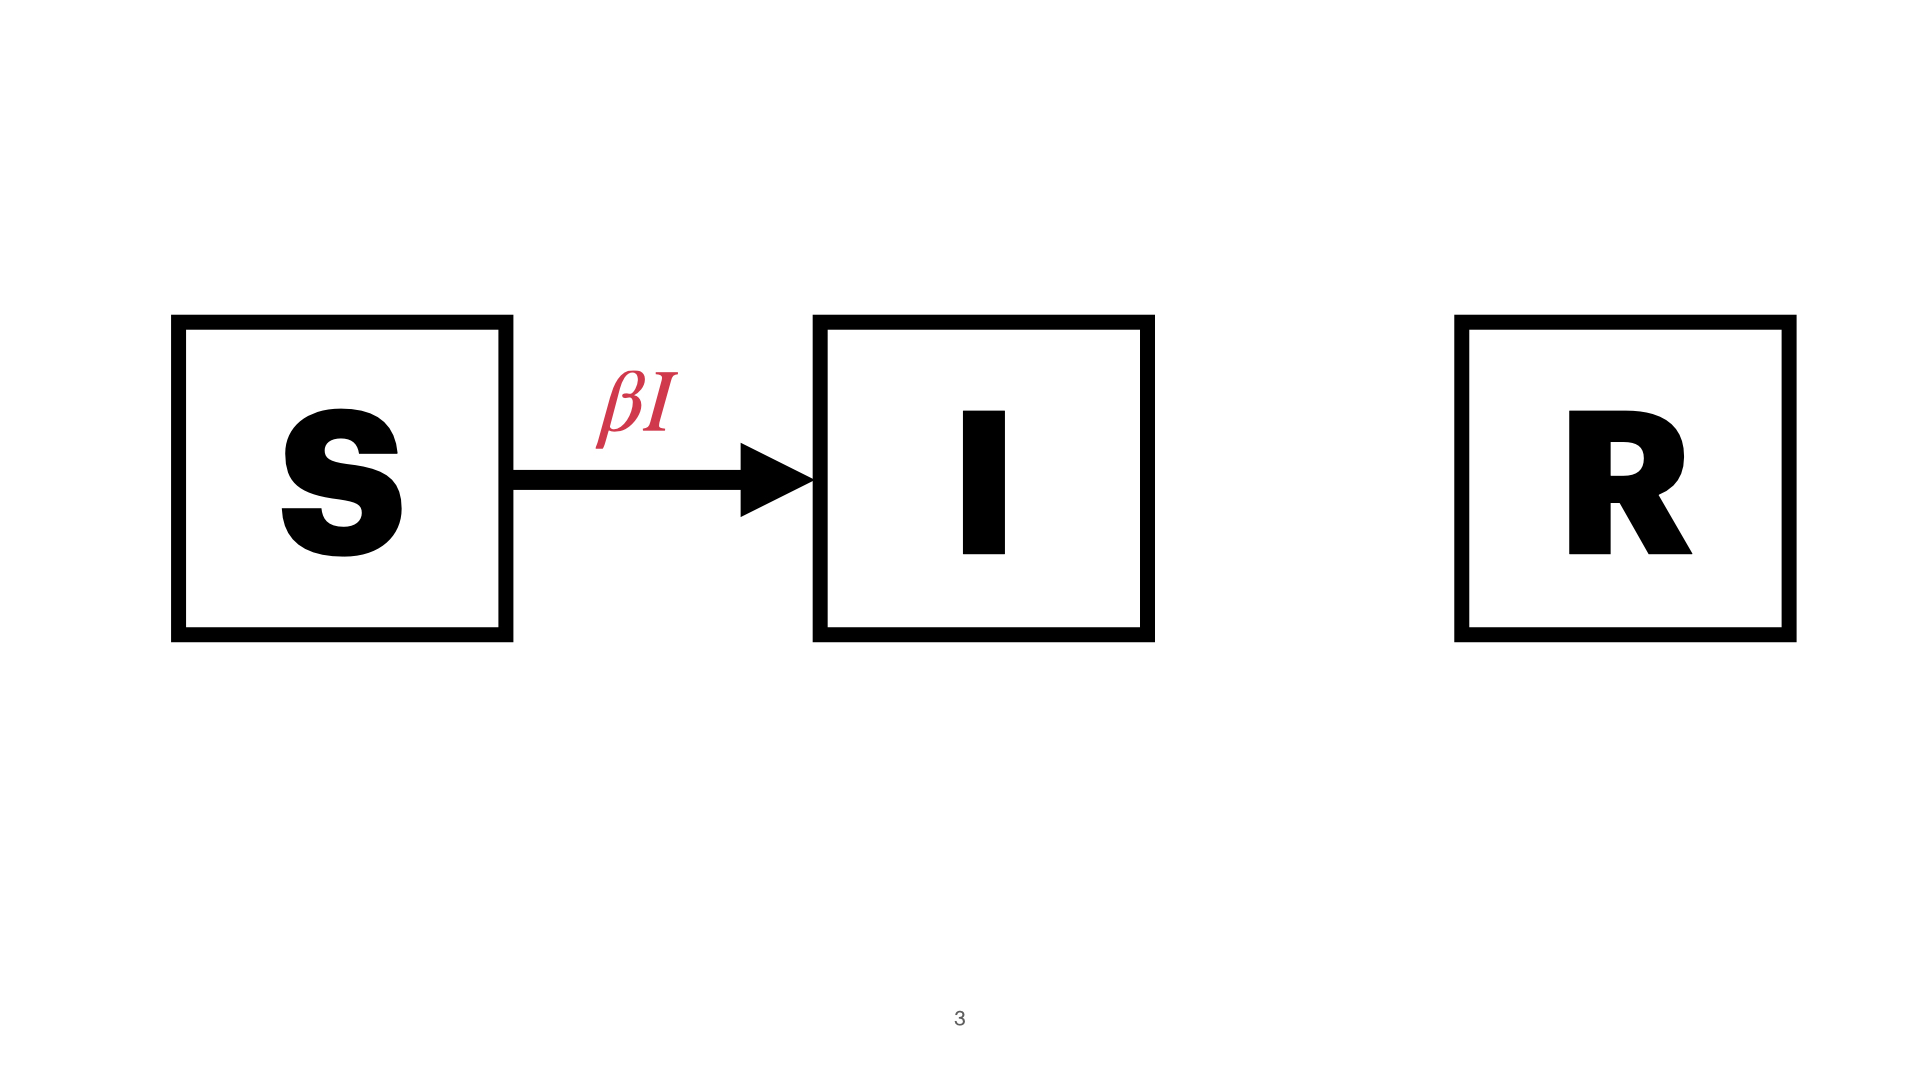
\includegraphics{images/model_diagrams/model_diagrams.003.jpeg}
\end{frame}

\begin{frame}
\begin{block}{Process 2: Recovery}
\phantomsection\label{process-2-recovery}
\begin{center}
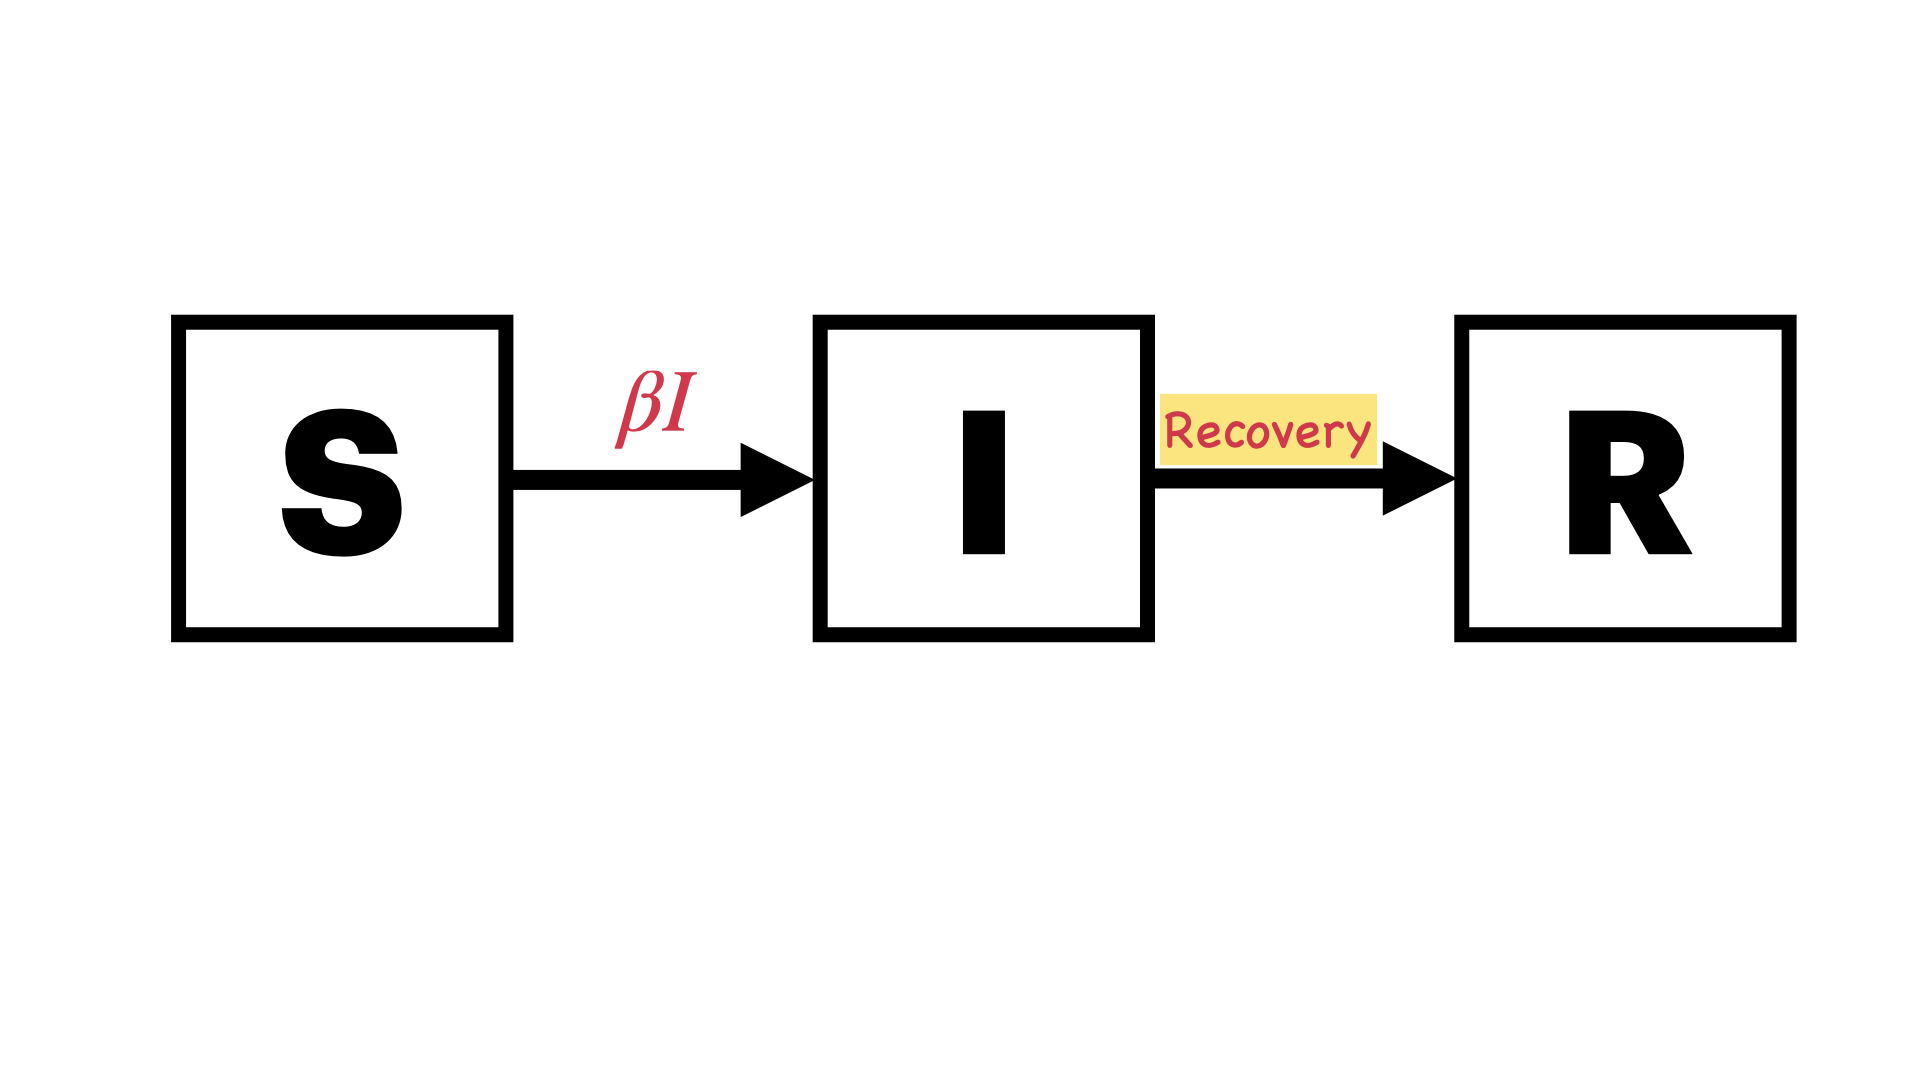
\includegraphics[width=0.6\textwidth,height=\textheight]{images/model_diagrams/model_diagrams.005.jpeg}
\end{center}

{Recovery}, governed by the recovery rate, \(\gamma\) (rate at which
infected individuals recover and become immune).
\end{block}
\end{frame}

\begin{frame}
\begin{block}{Some notes on the recovery process}
\phantomsection\label{some-notes-on-the-recovery-process}
\begin{itemize}
\item
  If the duration of infection is {\(\dfrac{1}{\gamma}\)}, then the rate
  at which infected individuals recover is {\(\gamma\)}.
\item
  The average infectious period is often {estimated from epidemiological
  data}.
\end{itemize}

\begin{tcolorbox}[enhanced jigsaw, colframe=quarto-callout-note-color-frame, toprule=.15mm, opacitybacktitle=0.6, breakable, colback=white, leftrule=.75mm, left=2mm, opacityback=0, titlerule=0mm, bottomtitle=1mm, toptitle=1mm, title={Note}, bottomrule=.15mm, arc=.35mm, coltitle=black, colbacktitle=quarto-callout-note-color!10!white, rightrule=.15mm]

You will learn about parameter estimation in the model fitting and
calibration lectures.

\end{tcolorbox}
\end{block}
\end{frame}

\begin{frame}
\begin{figure}[H]

{\centering 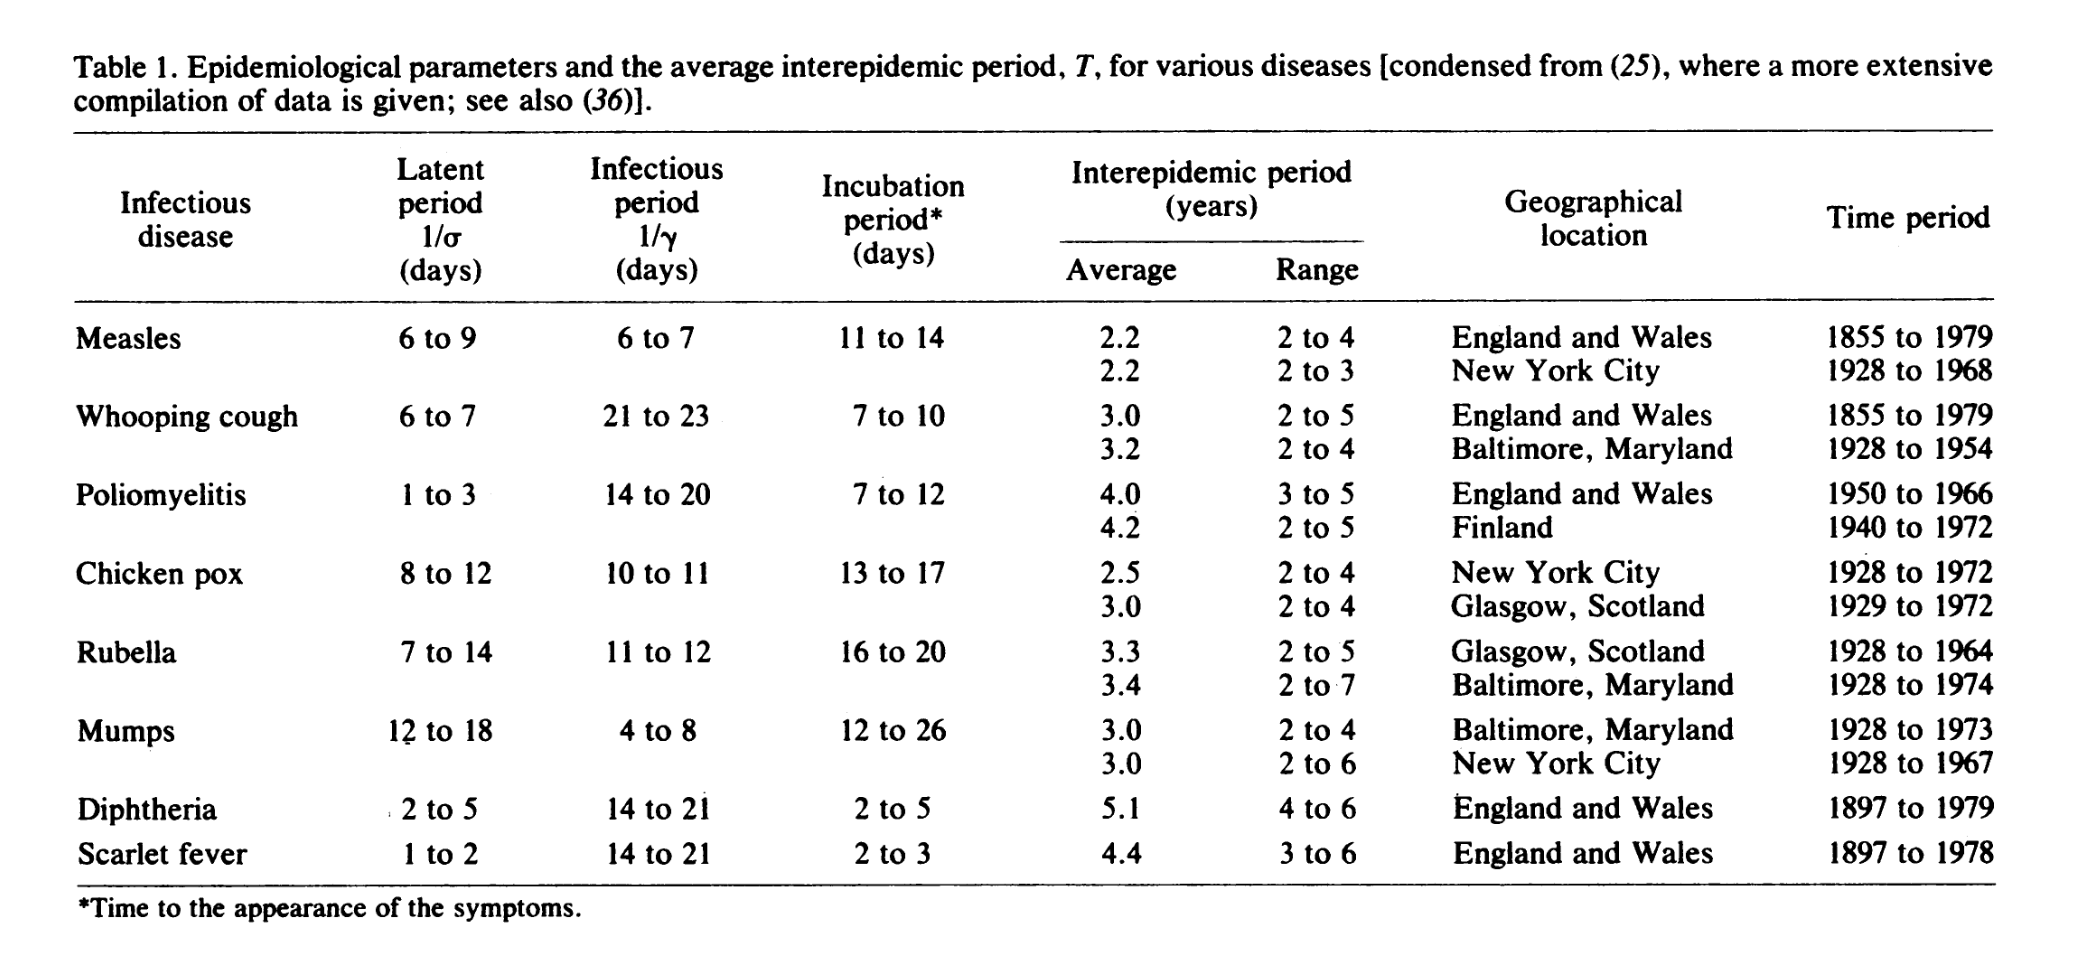
\includegraphics{images/epi_parameters.png}

}

\caption{Source:
(\citeproc{ref-anderson1982directly}{\textbf{anderson1982directly?}})}

\end{figure}%
\end{frame}

\begin{frame}
\begin{block}{Putting it all together}
\phantomsection\label{putting-it-all-together}
\begin{figure}[H]

{\centering 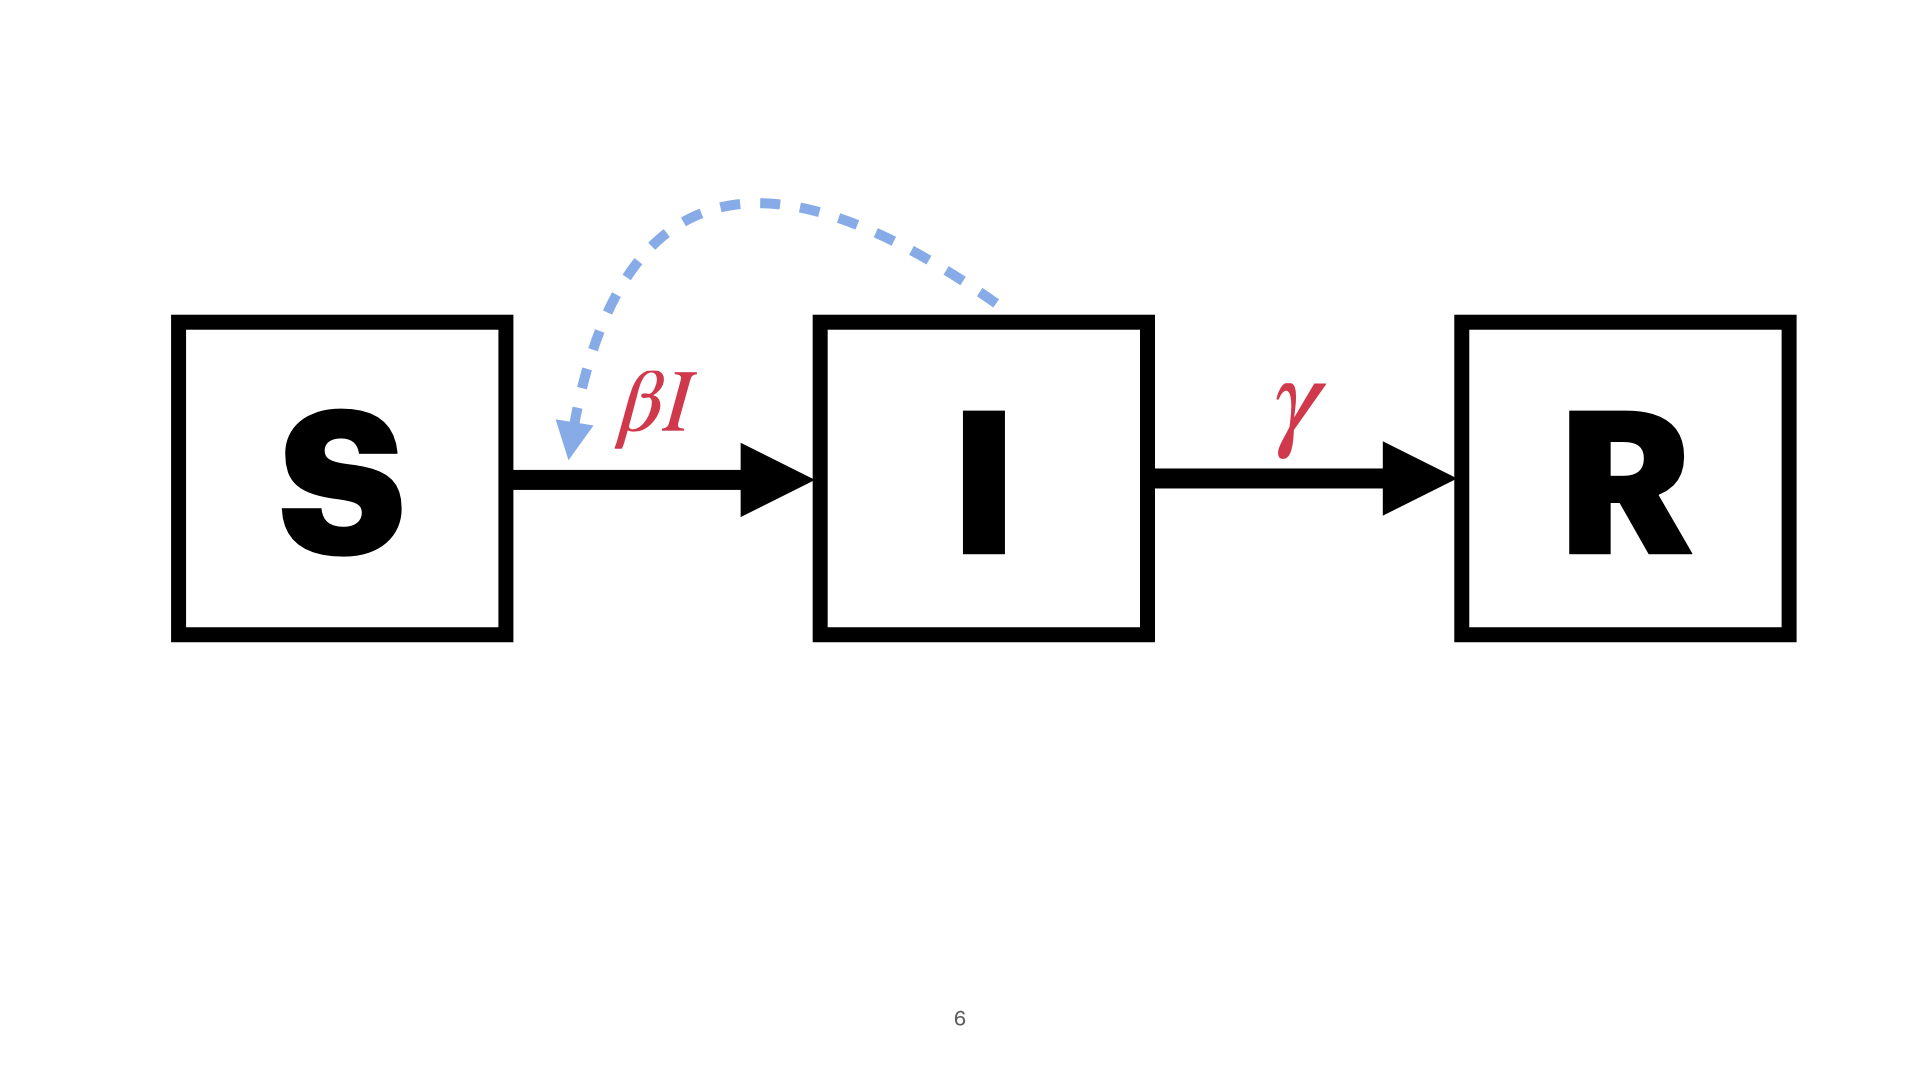
\includegraphics[width=0.8\textwidth,height=\textheight]{images/model_diagrams/model_diagrams.006.jpeg}

}

\caption{An SIR model with transmission rate, \(\beta\), and recovery
rate, \(\gamma\).}

\end{figure}%
\end{block}
\end{frame}

\begin{frame}
\begin{block}{Formulating the model equations}
\phantomsection\label{formulating-the-model-equations}
{Continuous time compartmental} models are formulated using
{differential equations} that describe the change in the number of
individuals in each compartment over time.
\end{block}
\end{frame}

\begin{frame}
The SIR model can be formulated as:

\begin{columns}[T]
\begin{column}{0.5\textwidth}
\begin{center}
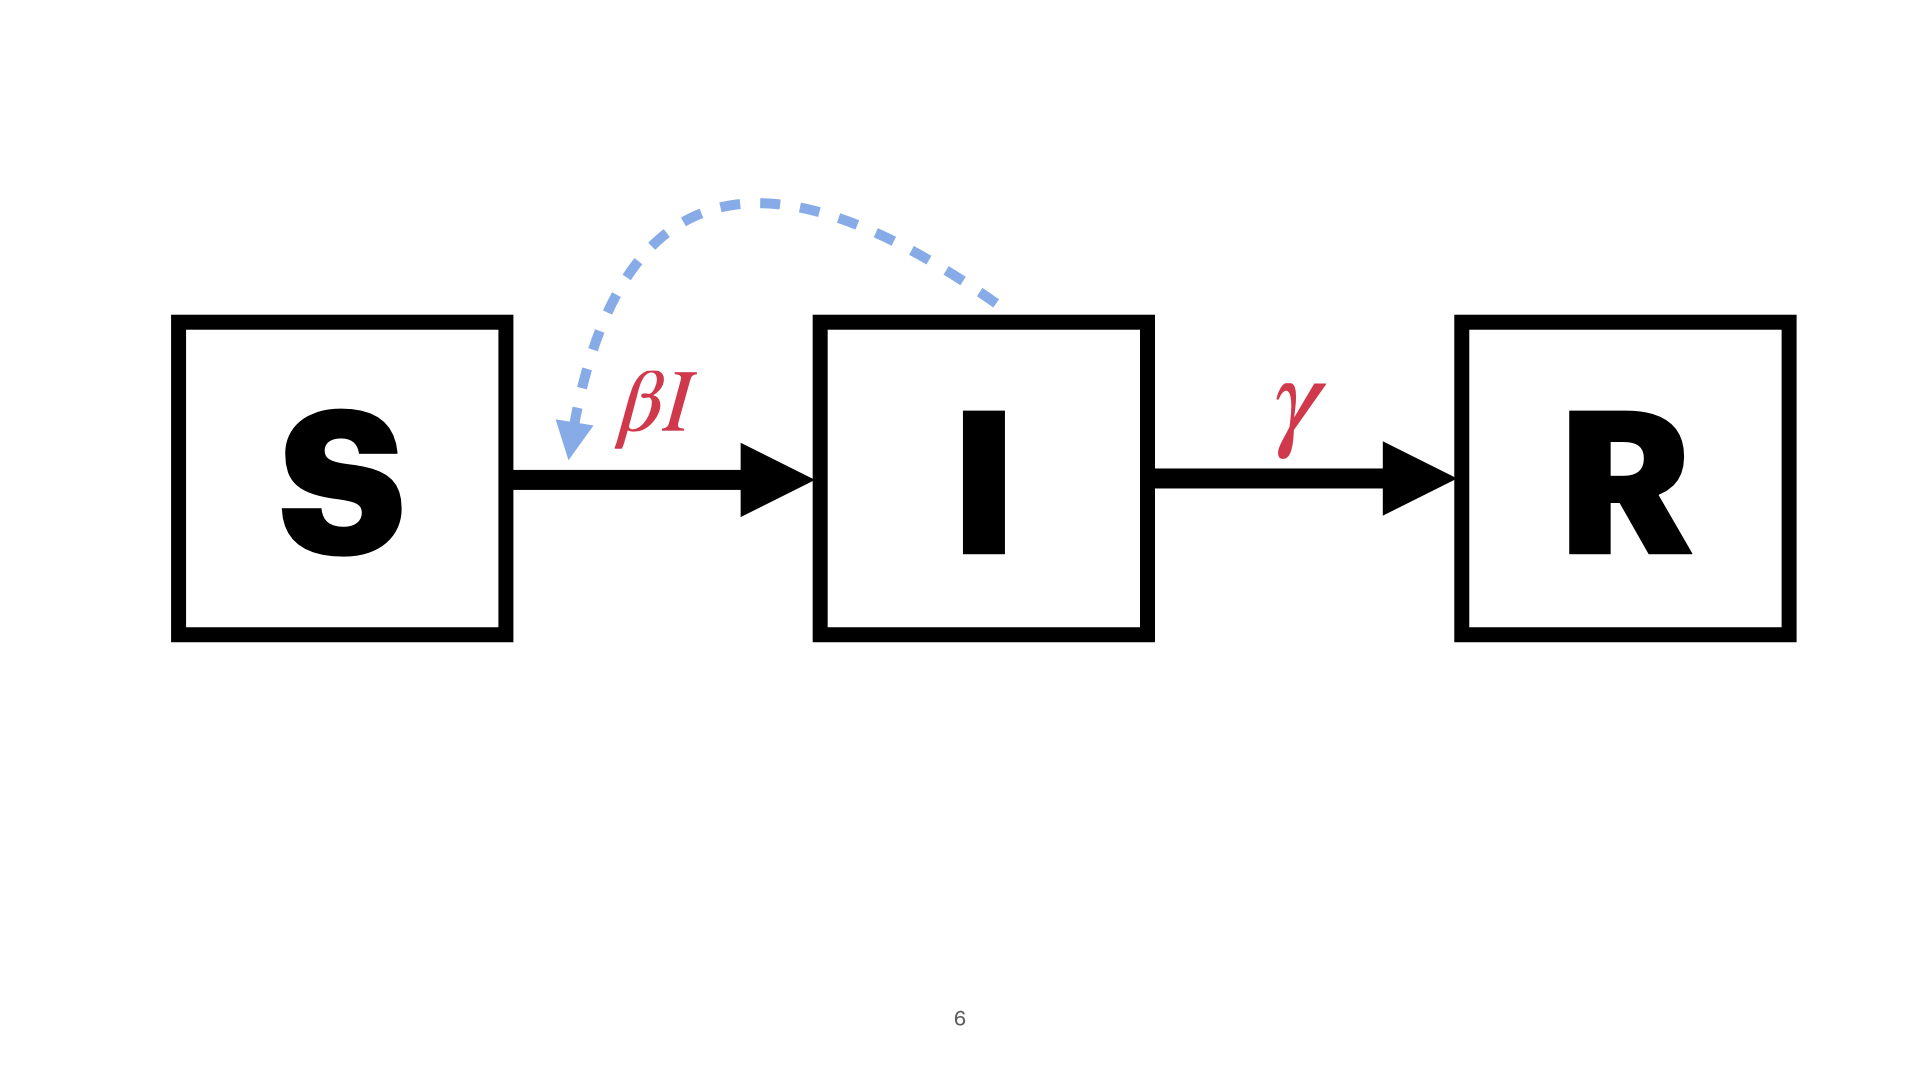
\includegraphics{images/model_diagrams/model_diagrams.006.jpeg}
\end{center}
\end{column}

\begin{column}{0.5\textwidth}
\begin{align*}
\frac{dS}{dt} & = \dot{S}  = \color{orange}{-\beta S I} \\
\frac{dI}{dt} & = \dot{I}  = \color{orange}{\beta S I} - \color{blue}{\gamma I} \\
\frac{dR}{dt} & = \dot{R} = \color{blue}{\gamma I}
\end{align*}
\end{column}
\end{columns}

where {\(\beta\)} is the transmission rate, and {\(\gamma\)} is the
recovery rate.

\note{\begin{itemize}
\tightlist
\item
  We may or may not use the dot notation to denote the rate of change.
\item
  The terms are just \textbf{inflows} and \textbf{outflows}.
\item
  \textbf{Pause} for questions and clarifications.
\end{itemize}}
\end{frame}

\begin{frame}
The initial conditions are given by:

\begin{equation*}
\begin{aligned}
S(0) & = N - 1,\\
I(0) & = 1, \text{and} \\
R(0) & = 0.
\end{aligned}
\end{equation*}

where \(N\) is the total population size.
\end{frame}

\begin{frame}
\begin{tcolorbox}[enhanced jigsaw, colframe=quarto-callout-note-color-frame, toprule=.15mm, opacitybacktitle=0.6, breakable, colback=white, leftrule=.75mm, left=2mm, opacityback=0, titlerule=0mm, bottomtitle=1mm, toptitle=1mm, title={Note}, bottomrule=.15mm, arc=.35mm, coltitle=black, colbacktitle=quarto-callout-note-color!10!white, rightrule=.15mm]

\begin{itemize}
\tightlist
\item
  We represent the compartments as {population sizes}.:

  \begin{itemize}
  \tightlist
  \item
    Some modellers often use {proportions} instead of population sizes
    as a way to remove the dimensions from the equations.
  \end{itemize}
\end{itemize}

\end{tcolorbox}
\end{frame}

\begin{frame}
\begin{block}{Model assumptions}
\phantomsection\label{model-assumptions}
\begin{itemize}
\tightlist
\item
  The population is closed: no births, deaths, or migration.

  \begin{itemize}
  \tightlist
  \item
    Implicitly: the epidemic occurs much faster than the time scale of
    births, deaths, or migration.
  \end{itemize}
\item
  Individuals are infectious immediately after infection and remain
  infectious until they recover.
\end{itemize}
\end{block}
\end{frame}

\begin{frame}
\begin{itemize}
\item
  Mixing is \emph{homogeneous}, i.e., {individuals mix randomly}:
\item
  Individuals have an equal probability of coming into contact with any
  other individual in the population.
\item
  Transition rates are constant and do not change over time.
\item
  Individuals acquire ``lifelong'' immunity after recovery.
\end{itemize}

\note{The \(R\) compartment is an absorbing state in this model.}
\end{frame}

\begin{frame}
\begin{tcolorbox}[enhanced jigsaw, colframe=quarto-callout-caution-color-frame, toprule=.15mm, opacitybacktitle=0.6, breakable, colback=white, leftrule=.75mm, left=2mm, opacityback=0, titlerule=0mm, bottomtitle=1mm, toptitle=1mm, title={Discussion}, bottomrule=.15mm, arc=.35mm, coltitle=black, colbacktitle=quarto-callout-caution-color!10!white, rightrule=.15mm]

\begin{itemize}
\tightlist
\item
  What diseases do you think the SIR model is appropriate for?
\end{itemize}

\end{tcolorbox}
\end{frame}

\begin{frame}
\begin{itemize}
\tightlist
\item
  The SIR model is appropriate for diseases that confer immunity after
  recovery. For example, measles and chicken pox.
\item
  Popularised by Kermack and McKendrick in 1927
  (\citeproc{ref-kermack1927contribution}{Kermack and McKendrick 1927})

  \begin{itemize}
  \tightlist
  \item
    A must-read paper for budding infectious disease modellers.
  \end{itemize}
\end{itemize}
\end{frame}

\begin{frame}
\begin{block}{What questions can we answer with the SIR model?}
\phantomsection\label{what-questions-can-we-answer-with-the-sir-model}
\begin{itemize}
\tightlist
\item
  The SIR model can be used to understand the dynamics of an epidemic:

  \begin{itemize}
  \tightlist
  \item
    How long will the epidemic last?
  \item
    How many individuals will be infected (final epidemic size)?
  \item
    When will the epidemic reach its peak?
  \end{itemize}
\end{itemize}
\end{block}
\end{frame}

\begin{frame}
\begin{block}{Solving the SIR model}
\phantomsection\label{solving-the-sir-model}
\begin{itemize}
\item
  Compartmental models cannot be solved analytically.
\item
  We often perform two types of analyses to understand the {long term
  dynamics} of the model:

  \begin{itemize}
  \tightlist
  \item
    Qualitative: threshold phenomena and analysis of equilibria
    (disease-free and endemic).\\
  \item
    Numerical simulations.
  \end{itemize}
\end{itemize}

\begin{tcolorbox}[enhanced jigsaw, colframe=quarto-callout-note-color-frame, toprule=.15mm, opacitybacktitle=0.6, breakable, colback=white, leftrule=.75mm, left=2mm, opacityback=0, titlerule=0mm, bottomtitle=1mm, toptitle=1mm, title=\textcolor{quarto-callout-note-color}{\faInfo}\hspace{0.5em}{Note}, bottomrule=.15mm, arc=.35mm, coltitle=black, colbacktitle=quarto-callout-note-color!10!white, rightrule=.15mm]

\begin{itemize}
\tightlist
\item
  For this introductory course, we will use focus on simulation.
\end{itemize}

\end{tcolorbox}

\begin{itemize}
\tightlist
\item
  But first, let's do some qualitative analysis of the SIR.
\end{itemize}
\end{block}
\end{frame}

\begin{frame}
\begin{block}{Threshold phenomena}
\phantomsection\label{threshold-phenomena}
\begin{itemize}
\tightlist
\item
  Here, we study the conditions under which an epidemic will {grow or
  die out} using the model equations.
\end{itemize}
\end{block}
\end{frame}

\begin{frame}
\begin{itemize}
\item
  Consider the case where \(I(0) = 1\) individual is introduced into a
  population of size \(N\) at time \(t = 0\).
\item
  That means in a completely susceptible population, we have
  \(S(0) = N - 1\) susceptible individuals.
\end{itemize}
\end{frame}

\begin{frame}
\begin{itemize}
\item
  At time 0, the disease will not spread if the rate of change of
  infections is negative, that is {\(\dfrac{dI}{dt} < 0\)}.
\item
  Recall from the SIR model that
  {\(\dfrac{dI}{dt} = \beta S I - \gamma I\)}.
\item
  Let's solve this equation at \(t = 0\) by setting \(I = 1\), assuming
  {\(\dfrac{dI}{dt} < 0\)}.
\end{itemize}
\end{frame}

\begin{frame}
At \(t = 0\), we have

\begin{equation*}
\frac{dI}{dt} = \beta S I - \gamma I < 0 \end{equation*}

Factor out \(I\), and we get

\begin{equation*}
I (\beta S - \gamma) < 0
\end{equation*}
\end{frame}

\begin{frame}
\begin{itemize}
\item
  Since at \(t=0\)\(, I > 0\), we have {\(S < \dfrac{\gamma}{\beta}\)}.
\item
  {\(\dfrac{\gamma}{\beta}\)} is the relative removal rate.
\end{itemize}
\end{frame}

\begin{frame}
\begin{itemize}
\item
  \textbf{Interpretation}:

  \begin{itemize}
  \tightlist
  \item
    At \(t = 0\), \(S\) must be less than \(\dfrac{\gamma}{\beta}\) for
    the epidemic to die out.
  \item
    If the rate of removal/recovery is greater than the transmission
    rate, the epidemic will die out.
  \item
    Any infection that cannot transmit to more than one host is going to
    die out.
  \end{itemize}
\end{itemize}
\end{frame}

\begin{frame}
For the SIR model, the quantity {\(\dfrac{\beta}{\gamma}\)} is called
the {reproduction number, \(R0\)} (pronounced ``R naught'' or ``R
zero'').
\end{frame}

\begin{frame}
\begin{block}{The basic reproduction number, R0}
\phantomsection\label{the-basic-reproduction-number-r0}
\begin{itemize}
\item
  The basic reproduction number, {\(R0\)}, is the average number of
  secondary infections generated by a {single primary infection} in a
  {completely susceptible} population.
\item
  The basic reproduction number is a key quantity in infectious disease
  epidemiology.
\end{itemize}
\end{block}
\end{frame}

\begin{frame}
\begin{itemize}
\tightlist
\item
  It is often represented as a single number or a range of high-low
  values.

  \begin{itemize}
  \tightlist
  \item
    For example, the \(R0\) for measles is popularly known to be \(12\)
    - \(18\)
    (\citeproc{ref-guerra2017measlesR0}{\textbf{guerra2017measlesR0?}}).
  \end{itemize}
\end{itemize}
\end{frame}

\begin{frame}
\begin{itemize}
\tightlist
\item
  \(R0\) is often used to express the threshold phenomena in infectious
  disease epidemiology:

  \begin{itemize}
  \tightlist
  \item
    If \(R0 > 1\), the epidemic will grow.
  \item
    If \(R0 < 1\), the epidemic will decline.
  \end{itemize}
\item
  A pathogen's \(R0\) value is determined by biological characteristics
  of the pathogen and the host's behaviour.
\end{itemize}
\end{frame}

\begin{frame}
\begin{itemize}
\tightlist
\item
  Conceptually, \(R0\) is given by
\end{itemize}

\[
R0 \propto \dfrac{\text{Infection}}{\text{Contact}} \times \dfrac{\text{Contact}}{\text{Time}} \times \dfrac{\text{Time}}{\text{Infection}}
\]

\begin{itemize}
\tightlist
\item
  \(R0\) is unitless and dimensionless.
\end{itemize}
\end{frame}

\begin{frame}
\begin{block}{Numerical simulations}
\phantomsection\label{numerical-simulations}
\begin{itemize}
\item
  Numerical simulations can be performed with any programming language.
\item
  This course focuses on the R programming language because:

  \begin{itemize}
  \tightlist
  \item
    It is a popular language for data analysis and statistical
    computing.
  \item
    It has a rich ecosystem of packages for solving differential
    equations.
  \item
    It is free and open-source.
  \end{itemize}
\end{itemize}
\end{block}
\end{frame}

\begin{frame}[fragile]
\begin{itemize}
\item
  In R, we can use the \texttt{\{deSolve\}} package to solve the
  differential equations.
\item
  To solve the model in R with \texttt{\{deSolve\}}, we will always need
  to define at least three things:

  \begin{itemize}
  \tightlist
  \item
    The model equations.
  \item
    The initial parameter values.
  \item
    The initial conditions (population sizes).
  \end{itemize}
\end{itemize}
\end{frame}

\begin{frame}[fragile]
\begin{block}{Practicals}
\phantomsection\label{practicals}
\begin{itemize}
\tightlist
\item
  Let's do a code walk through in R using the script \texttt{sir.Rmd}.
\end{itemize}
\end{block}
\end{frame}

\begin{frame}
\begin{tcolorbox}[enhanced jigsaw, colframe=quarto-callout-caution-color-frame, toprule=.15mm, opacitybacktitle=0.6, breakable, colback=white, leftrule=.75mm, left=2mm, opacityback=0, titlerule=0mm, bottomtitle=1mm, toptitle=1mm, title={Discussion}, bottomrule=.15mm, arc=.35mm, coltitle=black, colbacktitle=quarto-callout-caution-color!10!white, rightrule=.15mm]

\begin{itemize}
\tightlist
\item
  What happens if we increase or decrease the value of \(R0\)?
\item
  What happens if we increase or decrease the value of the infectious
  period?
\item
  How can we flatten the curve?
\end{itemize}

\end{tcolorbox}

\note{\begin{itemize}
\tightlist
\item
  We can flatten the curve by reducing the value of \(R0\).
\item
  In reality, we can reduce \(R0\) by implementing control measures such
  as social distancing, wearing masks, and vaccination.
\item
  These control measures reduce the number of contacts between
  individuals or the probability of infection, which in turn reduces the
  transmission rate.
\end{itemize}}
\end{frame}

\begin{frame}
\begin{block}{The Susceptible-Exposed-Infected-Recovered (SEIR) Model}
\phantomsection\label{the-susceptible-exposed-infected-recovered-seir-model}
\begin{figure}[H]

{\centering 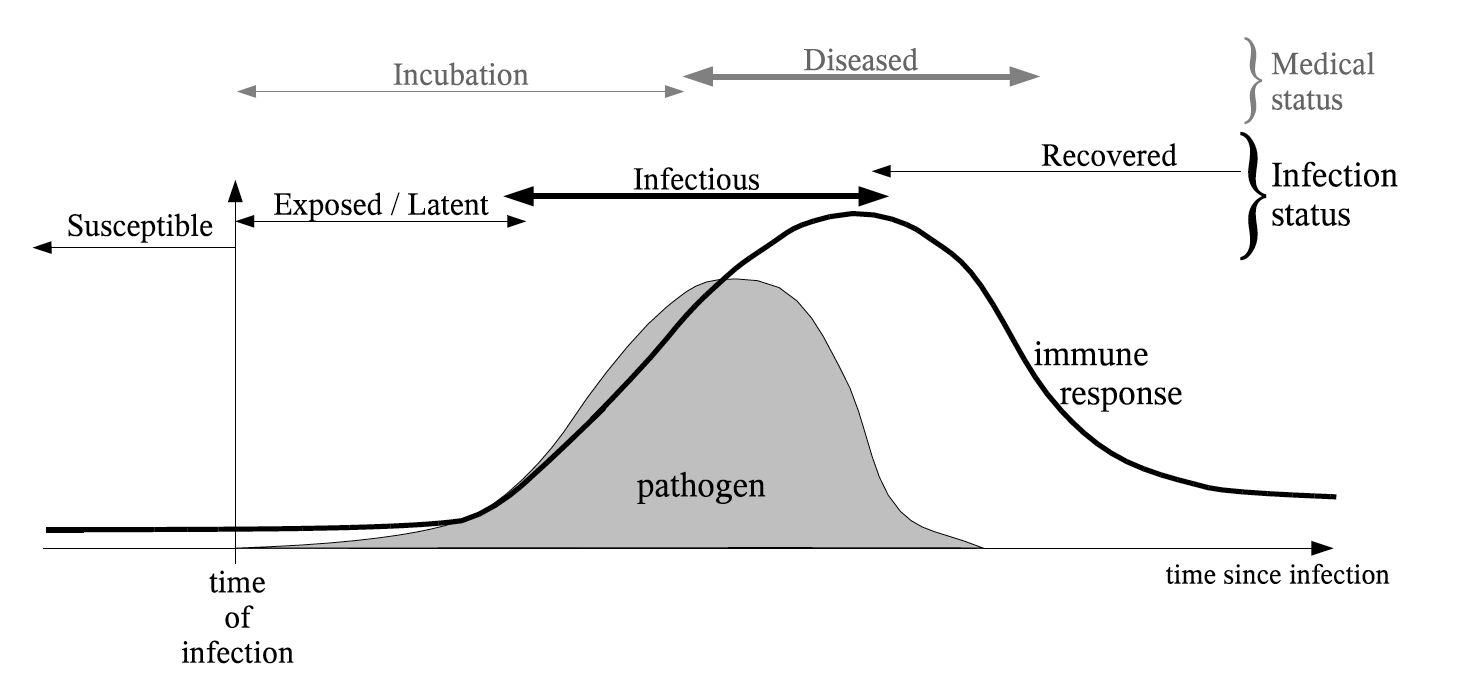
\includegraphics{images/infection_timeline.png}

}

\caption{Timeline of infection. Source: Keeling \& Rohani, 2008}

\end{figure}%
\end{block}
\end{frame}

\begin{frame}
\begin{columns}[T]
\begin{column}{0.3\textwidth}
\begin{figure}[H]

{\centering \includegraphics{images/corona_virus.jpeg}

}

\caption{The SARS-COV-2 virus}

\end{figure}%%
\begin{figure}[H]

{\centering \includegraphics{images/ebola_virus.jpeg}

}

\caption{The Ebola virus}

\end{figure}%
\end{column}

\begin{column}{0.7\textwidth}
\begin{itemize}
\tightlist
\item
  Some diseases have an {latent/exposed period} during which individuals
  are {infected but not yet infectious}. Examples include pertussis,
  COVID-19, and Ebola.
\item
  Disease transmission does not occur during the latent period because
  of low levels of the virus in the host.
\end{itemize}
\end{column}
\end{columns}
\end{frame}

\begin{frame}
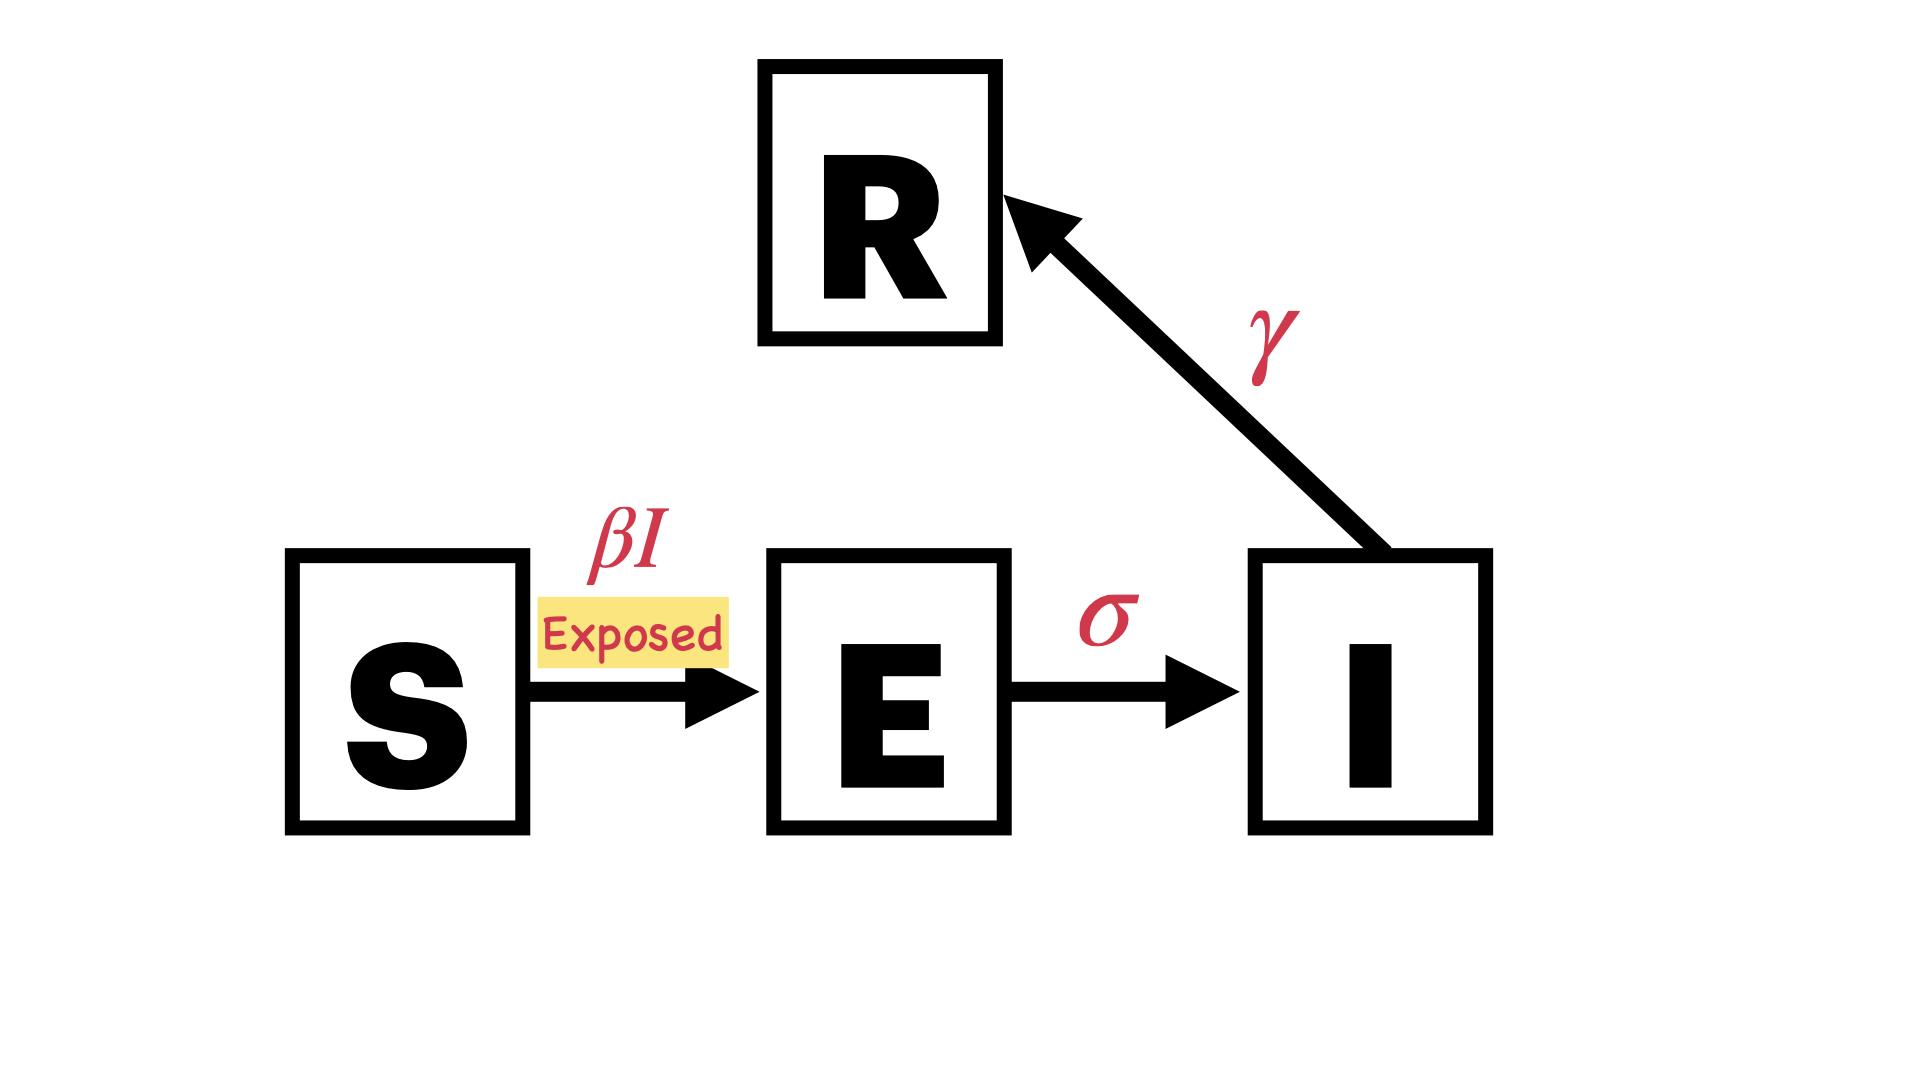
\includegraphics{images/model_diagrams/model_diagrams.007.jpeg}
\end{frame}

\begin{frame}
\begin{columns}[T]
\begin{column}{0.5\textwidth}
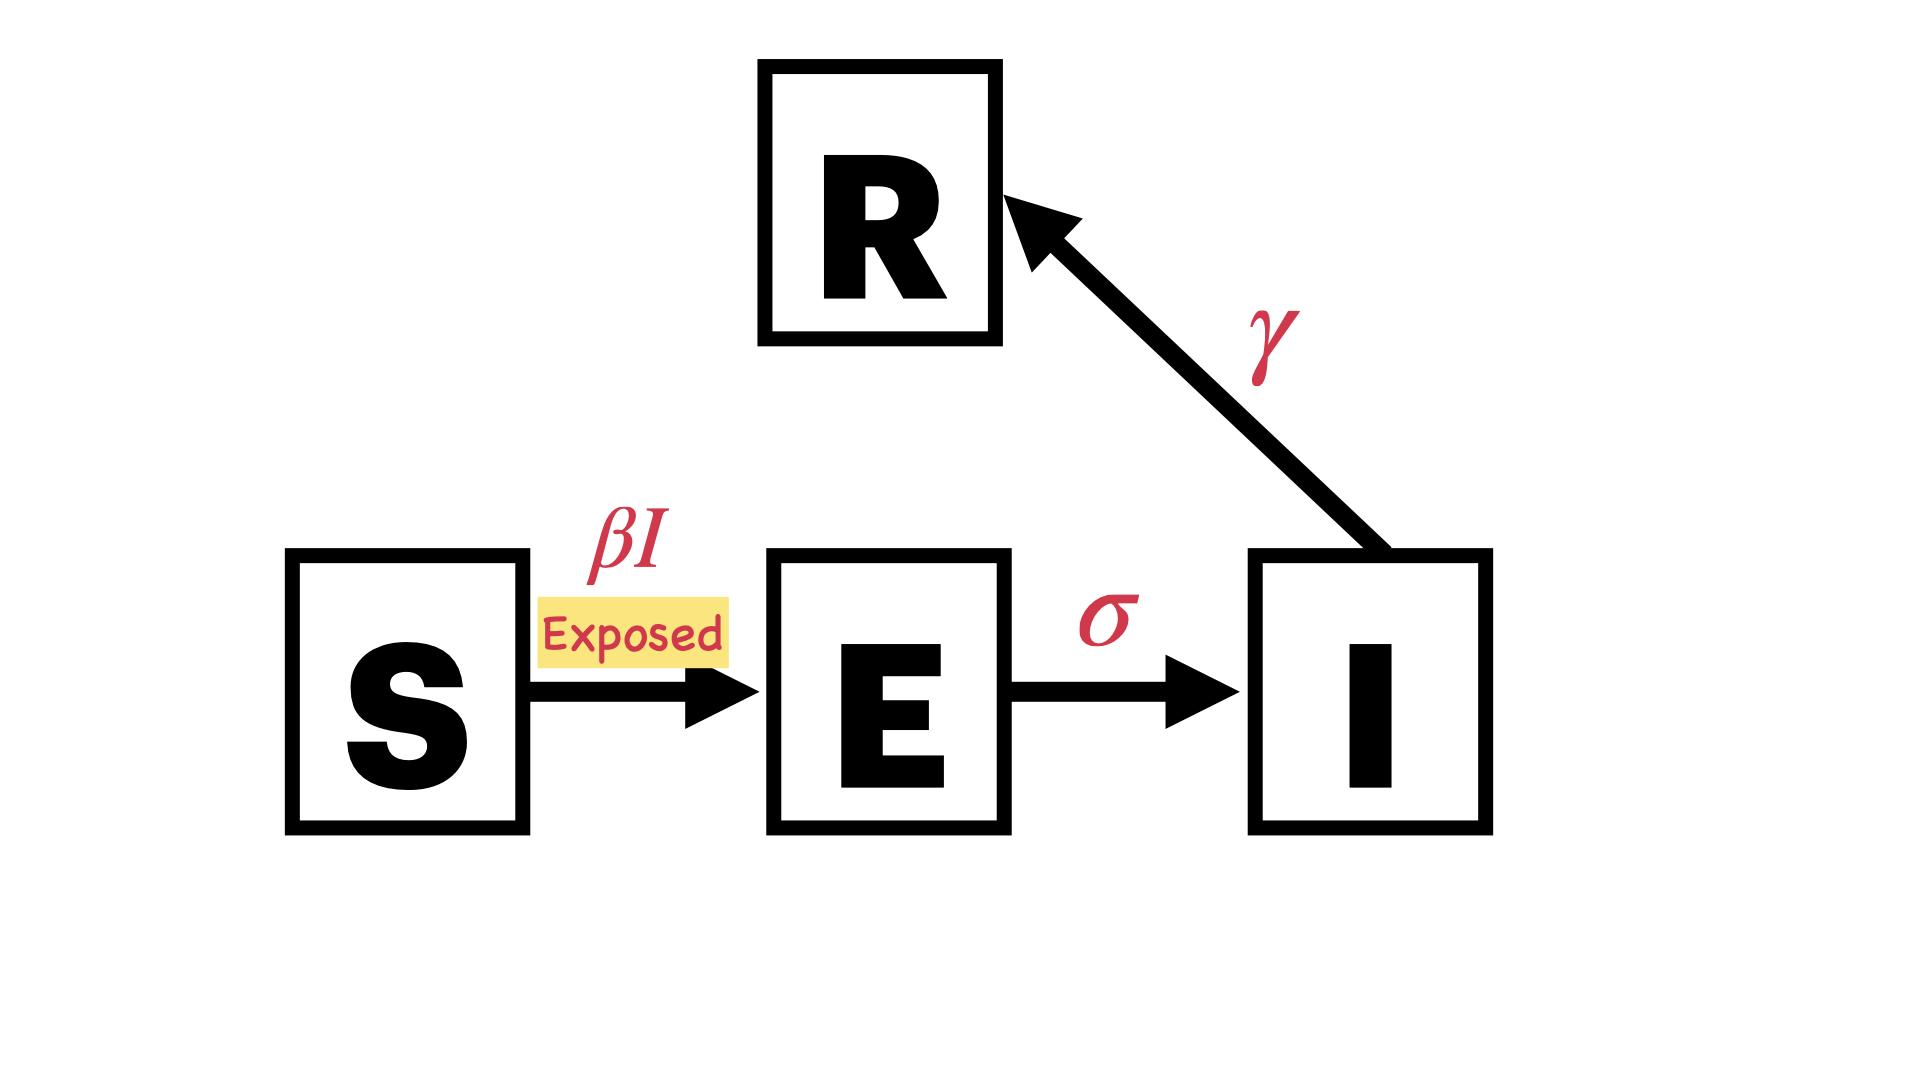
\includegraphics{images/model_diagrams/model_diagrams.007.jpeg}
\end{column}

\begin{column}{0.5\textwidth}
\begin{itemize}
\tightlist
\item
  The SEIR model extends the SIR model to include an exposed
  compartment, {\(E\)}.
\item
  {\(E\)}: infected but are not yet infectious.
\item
  Individuals stay in {\(E\)} for {\(1/\sigma\)} days before moving to
  \(I\).
\end{itemize}
\end{column}
\end{columns}
\end{frame}

\begin{frame}
\begin{columns}[T]
\begin{column}{0.6\textwidth}
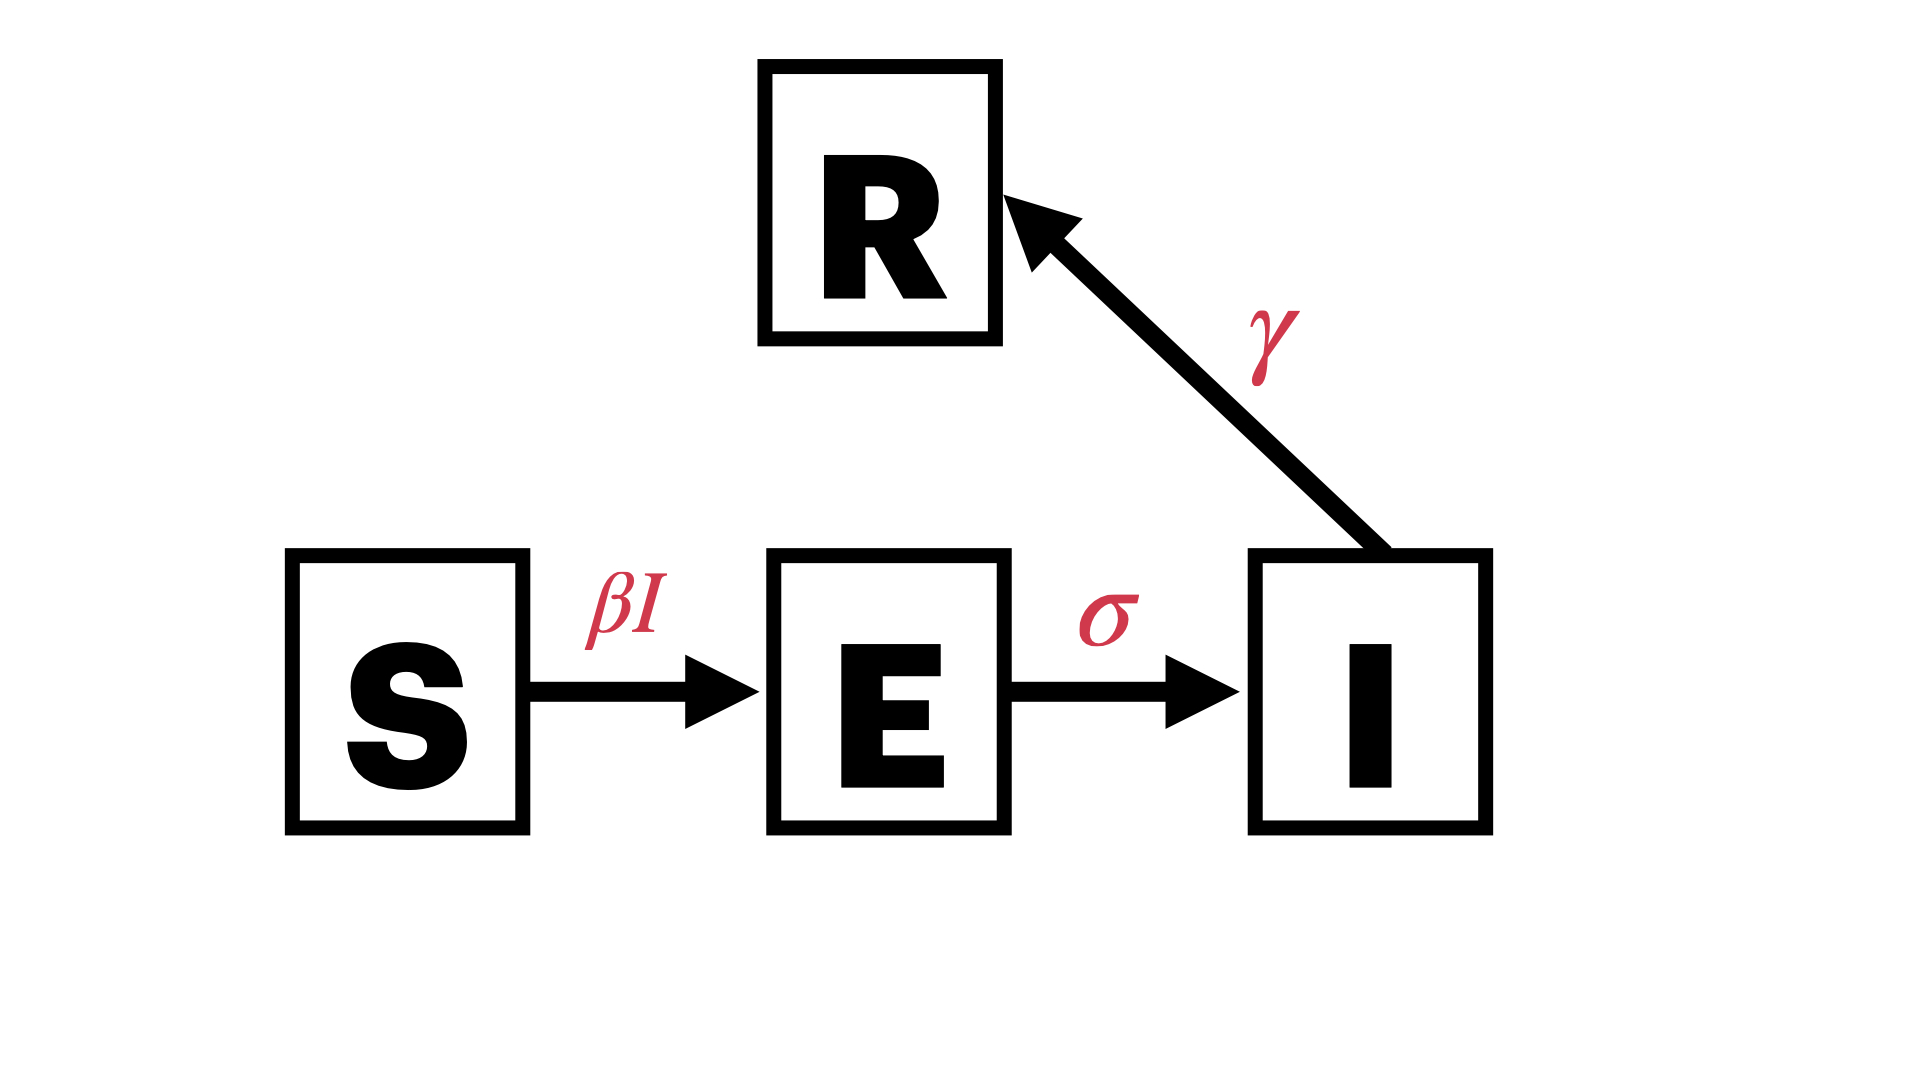
\includegraphics[width=0.8\textwidth,height=\textheight]{images/model_diagrams/model_diagrams.008.jpeg}
\end{column}

\begin{column}{0.4\textwidth}
Model equations: \begin{align*}
\frac{dS}{dt} & = -\beta S I \\
\frac{dE}{dt} & = \beta S I - \color{orange}{\sigma E} \\
\frac{dI}{dt} & = \color{orange}{\sigma E} - \gamma I \\
\frac{dR}{dt} & = \gamma I
\end{align*}
\end{column}
\end{columns}
\end{frame}

\begin{frame}
\begin{block}{SEIR model with births and deaths}
\phantomsection\label{seir-model-with-births-and-deaths}
\begin{itemize}
\item
  Let's relax the assumption about births and deaths in the population.
\item
  We will assume that the susceptible population is replenished with new
  individuals at a constant rate, \(\mu\).
\item
  We will also assume that everyone dies at a constant rate, \(\mu\).
\end{itemize}
\end{block}
\end{frame}

\begin{frame}
Our model schematic now looks like this:

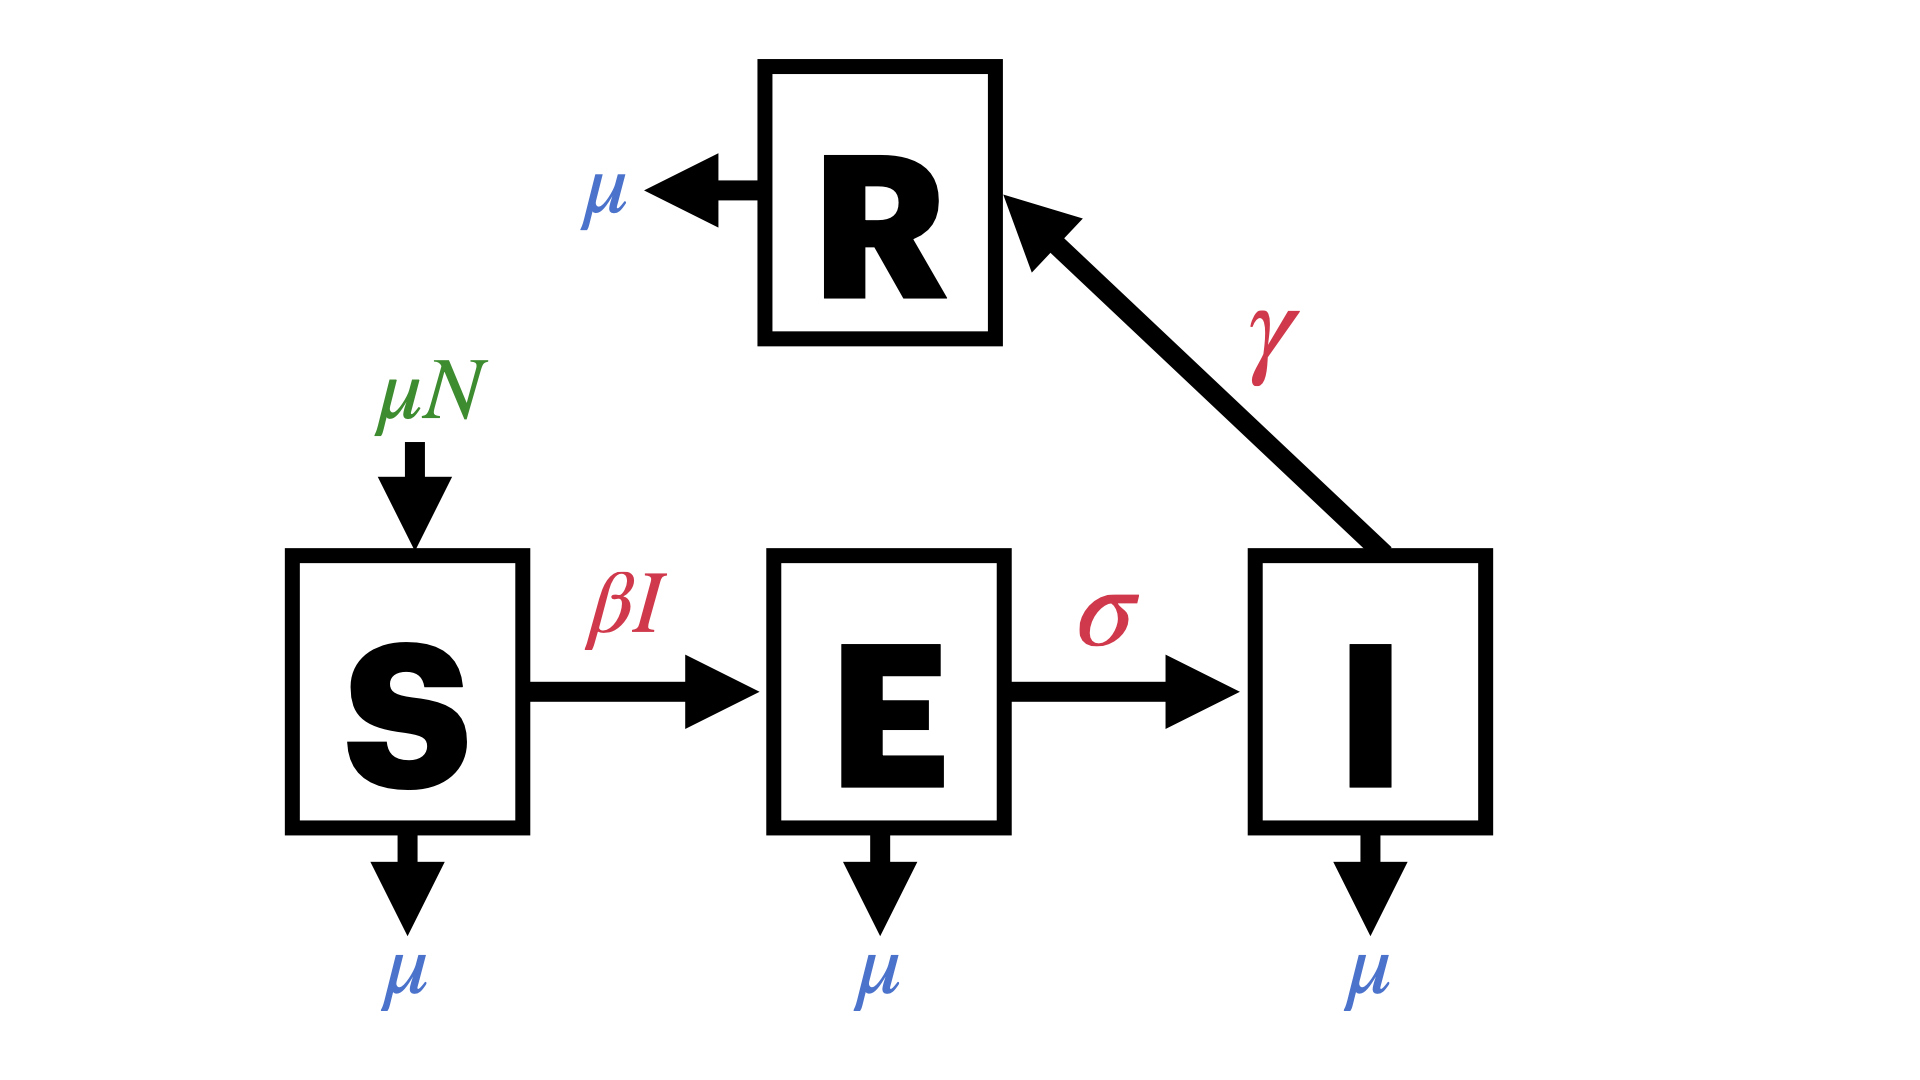
\includegraphics{images/model_diagrams/model_diagrams.009.jpeg}

\note{Explain in terms of inflows and outflows}
\end{frame}

\begin{frame}
\begin{columns}[T]
\begin{column}{0.5\textwidth}
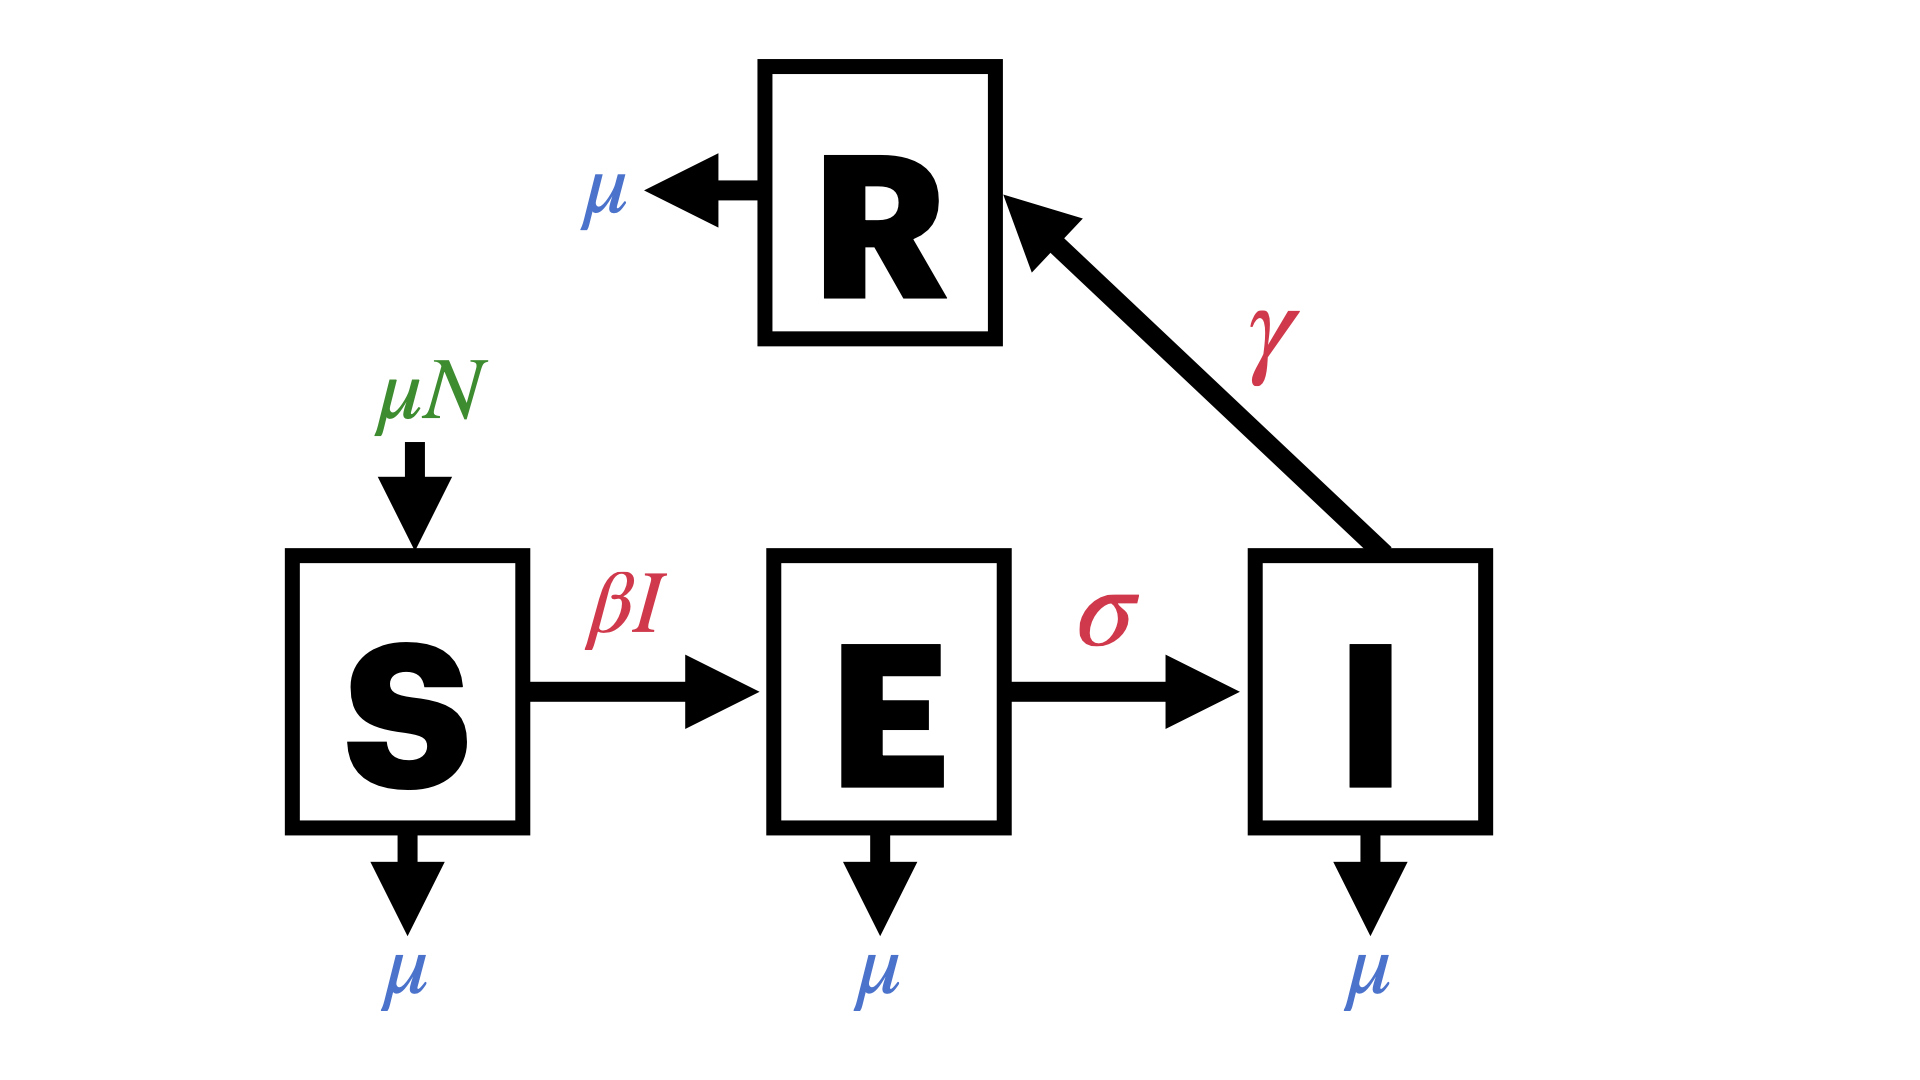
\includegraphics{images/model_diagrams/model_diagrams.009.jpeg}
\end{column}

\begin{column}{0.5\textwidth}
The model equations now become:

\begin{align}
\frac{dS}{dt} & = \color{green}{\mu N} - \beta S I - \color{blue}{\mu} S \\
\frac{dE}{dt} & = \beta S I - \sigma E - \color{blue}{\mu} E \\
\frac{dI}{dt} & = \sigma E - \gamma I - \color{blue}{\mu} I \\
\frac{dR}{dt} & = \gamma I - \color{blue}{\mu} R
\end{align}
\end{column}
\end{columns}
\end{frame}

\begin{frame}
\begin{tcolorbox}[enhanced jigsaw, colframe=quarto-callout-caution-color-frame, toprule=.15mm, opacitybacktitle=0.6, breakable, colback=white, leftrule=.75mm, left=2mm, opacityback=0, titlerule=0mm, bottomtitle=1mm, toptitle=1mm, title={Discussion}, bottomrule=.15mm, arc=.35mm, coltitle=black, colbacktitle=quarto-callout-caution-color!10!white, rightrule=.15mm]

What is the \(R0\) of the SEIR model?

\end{tcolorbox}
\end{frame}

\begin{frame}
\begin{block}{The R0 of the SEIR Model}
\phantomsection\label{the-r0-of-the-seir-model}
\begin{itemize}
\item
  Beyond the SIR model, calculating \(R0\) for more complex models can
  be challenging due to the presence of multiple compartments.
\item
  For complex models, we use the {next generation matrix} approach
  (\citeproc{ref-diekmann1990definition}{\textbf{diekmann1990definition?}};
  \citeproc{ref-diekmann2010construction}{\textbf{diekmann2010construction?}}).
\end{itemize}

\begin{tcolorbox}[enhanced jigsaw, colframe=quarto-callout-note-color-frame, toprule=.15mm, opacitybacktitle=0.6, breakable, colback=white, leftrule=.75mm, left=2mm, opacityback=0, titlerule=0mm, bottomtitle=1mm, toptitle=1mm, title={Note}, bottomrule=.15mm, arc=.35mm, coltitle=black, colbacktitle=quarto-callout-note-color!10!white, rightrule=.15mm]

Using the next generation matrix approach, we can show that the SEIR
model with constant births and deaths has
\[R0 = \dfrac{\beta \sigma}{(\gamma + \mu)(\sigma + \mu)}\].

\end{tcolorbox}
\end{block}
\end{frame}

\begin{frame}[fragile]
\begin{block}{Numerical simulations}
\phantomsection\label{numerical-simulations-1}
\begin{block}{R Practicals}
\phantomsection\label{r-practicals}
\begin{itemize}
\item
  We can use the same approach as the SIR model to simulate the SEIR
  model.
\item
  Modify the \texttt{sir.Rmd} script to simulate the SEIR model.
\end{itemize}
\end{block}
\end{block}
\end{frame}

\begin{frame}{Modelling epidemic control}
\phantomsection\label{modelling-epidemic-control}
\begin{tcolorbox}[enhanced jigsaw, colframe=quarto-callout-note-color-frame, toprule=.15mm, opacitybacktitle=0.6, breakable, colback=white, leftrule=.75mm, left=2mm, opacityback=0, titlerule=0mm, bottomtitle=1mm, toptitle=1mm, title=\textcolor{quarto-callout-note-color}{\faInfo}\hspace{0.5em}{Note}, bottomrule=.15mm, arc=.35mm, coltitle=black, colbacktitle=quarto-callout-note-color!10!white, rightrule=.15mm]

For a recap on the various control measures, refer to
Section~\ref{sec-control-measures}.

\end{tcolorbox}
\end{frame}

\begin{frame}
\begin{block}{Vaccination}
\phantomsection\label{vaccination}
For a background on vaccination, refer to Section~\ref{sec-vaccination}.
\end{block}
\end{frame}

\begin{frame}
\begin{columns}[T]
\begin{column}{0.4\textwidth}
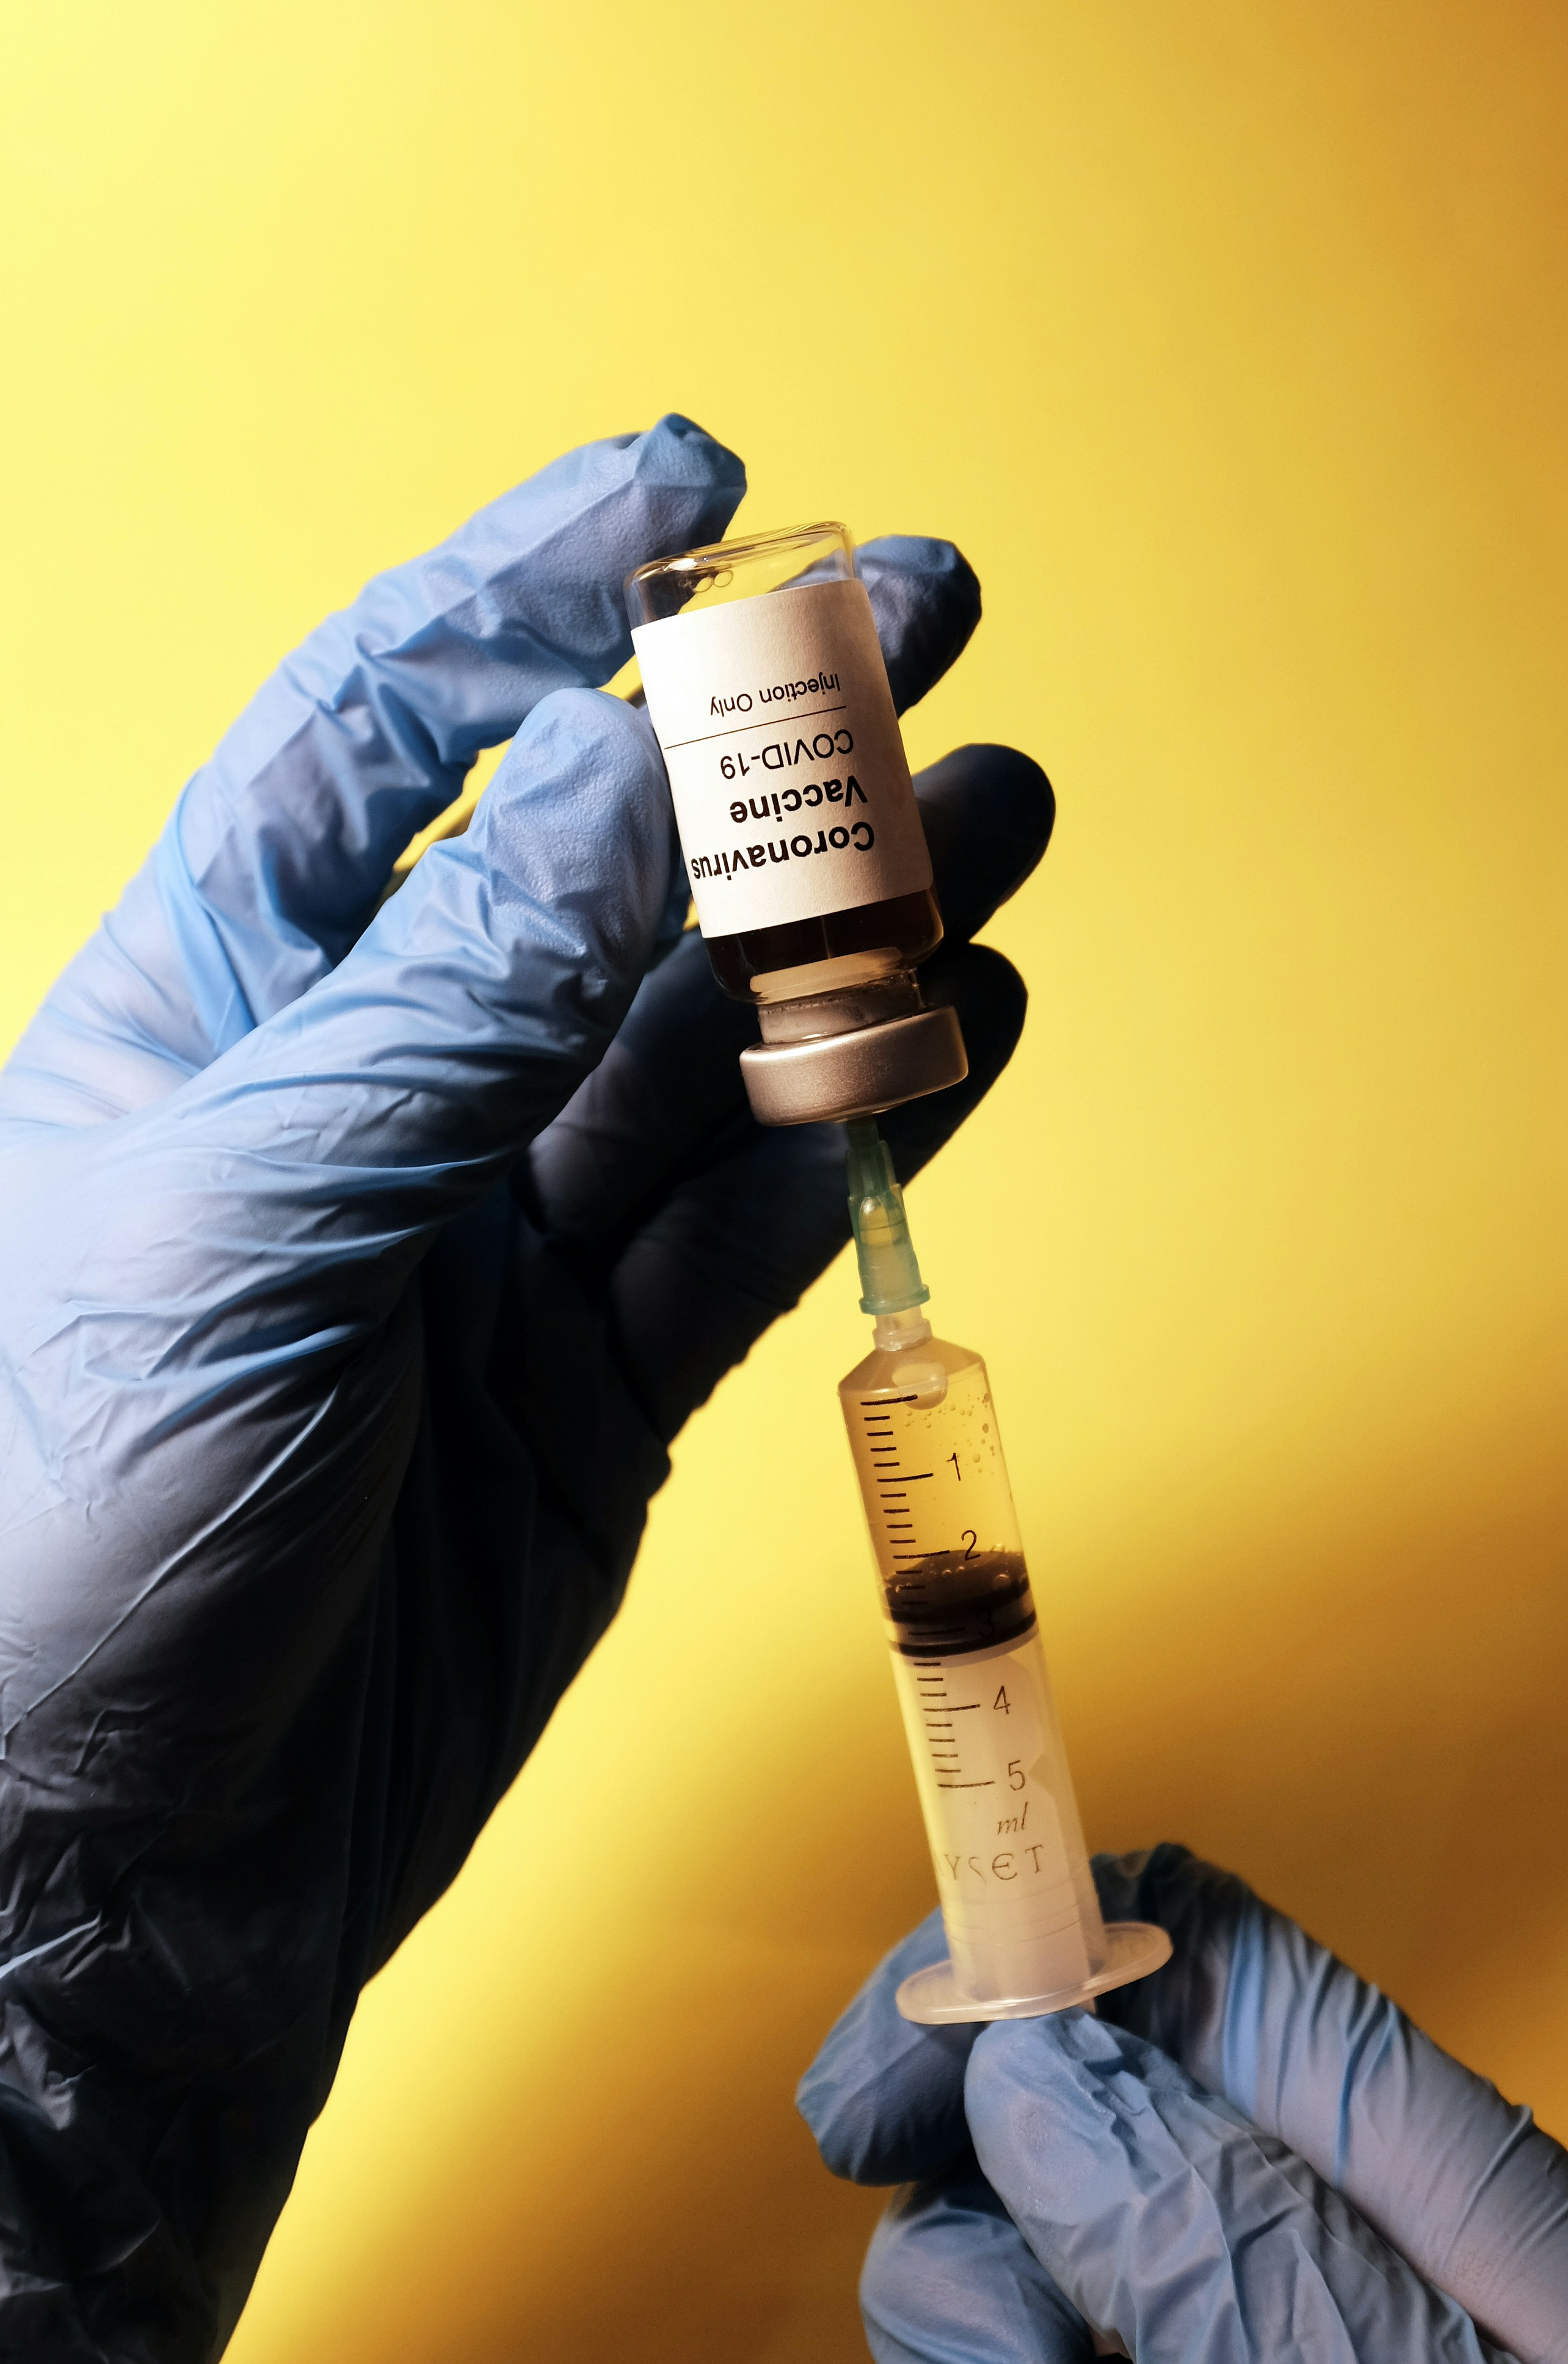
\includegraphics[width=1\textwidth,height=\textheight]{images/vaccine.jpeg}
\end{column}

\begin{column}{0.6\textwidth}
\begin{itemize}
\tightlist
\item
  Vaccination is one of the most effective ways to control infectious
  diseases.
\item
  Conceptually, vaccination works to reduce the number of susceptible
  individuals, \(S\).
\end{itemize}
\end{column}
\end{columns}
\end{frame}

\begin{frame}
\begin{itemize}
\item
  There are different types of vaccination strategies, including:

  \begin{itemize}
  \tightlist
  \item
    {pediatric} vaccination: vaccinating children to prevent the spread
    of diseases.
  \item
    {mass/random} vaccination: vaccinating a large proportion of the
    population.
  \item
    {targeted} vaccination: vaccinating specific groups of individuals,
    example, healthcare workers.
  \item
    {pulse} vaccination: periodically vaccinating a large number of
    individuals.
  \end{itemize}
\end{itemize}
\end{frame}

\begin{frame}
\begin{itemize}
\item
  Let's consider the case of mass/random vaccination.
\item
  Compartmental models can be extended to capture this by adding a new
  compartment, \(V\).
\item
  Let's consider the SEIR model with vaccination.
\end{itemize}
\end{frame}

\begin{frame}
\begin{block}{The Susceptible-Exposed-Infected-Recovered-Vaccinated
(SEIRV) Model}
\phantomsection\label{the-susceptible-exposed-infected-recovered-vaccinated-seirv-model}
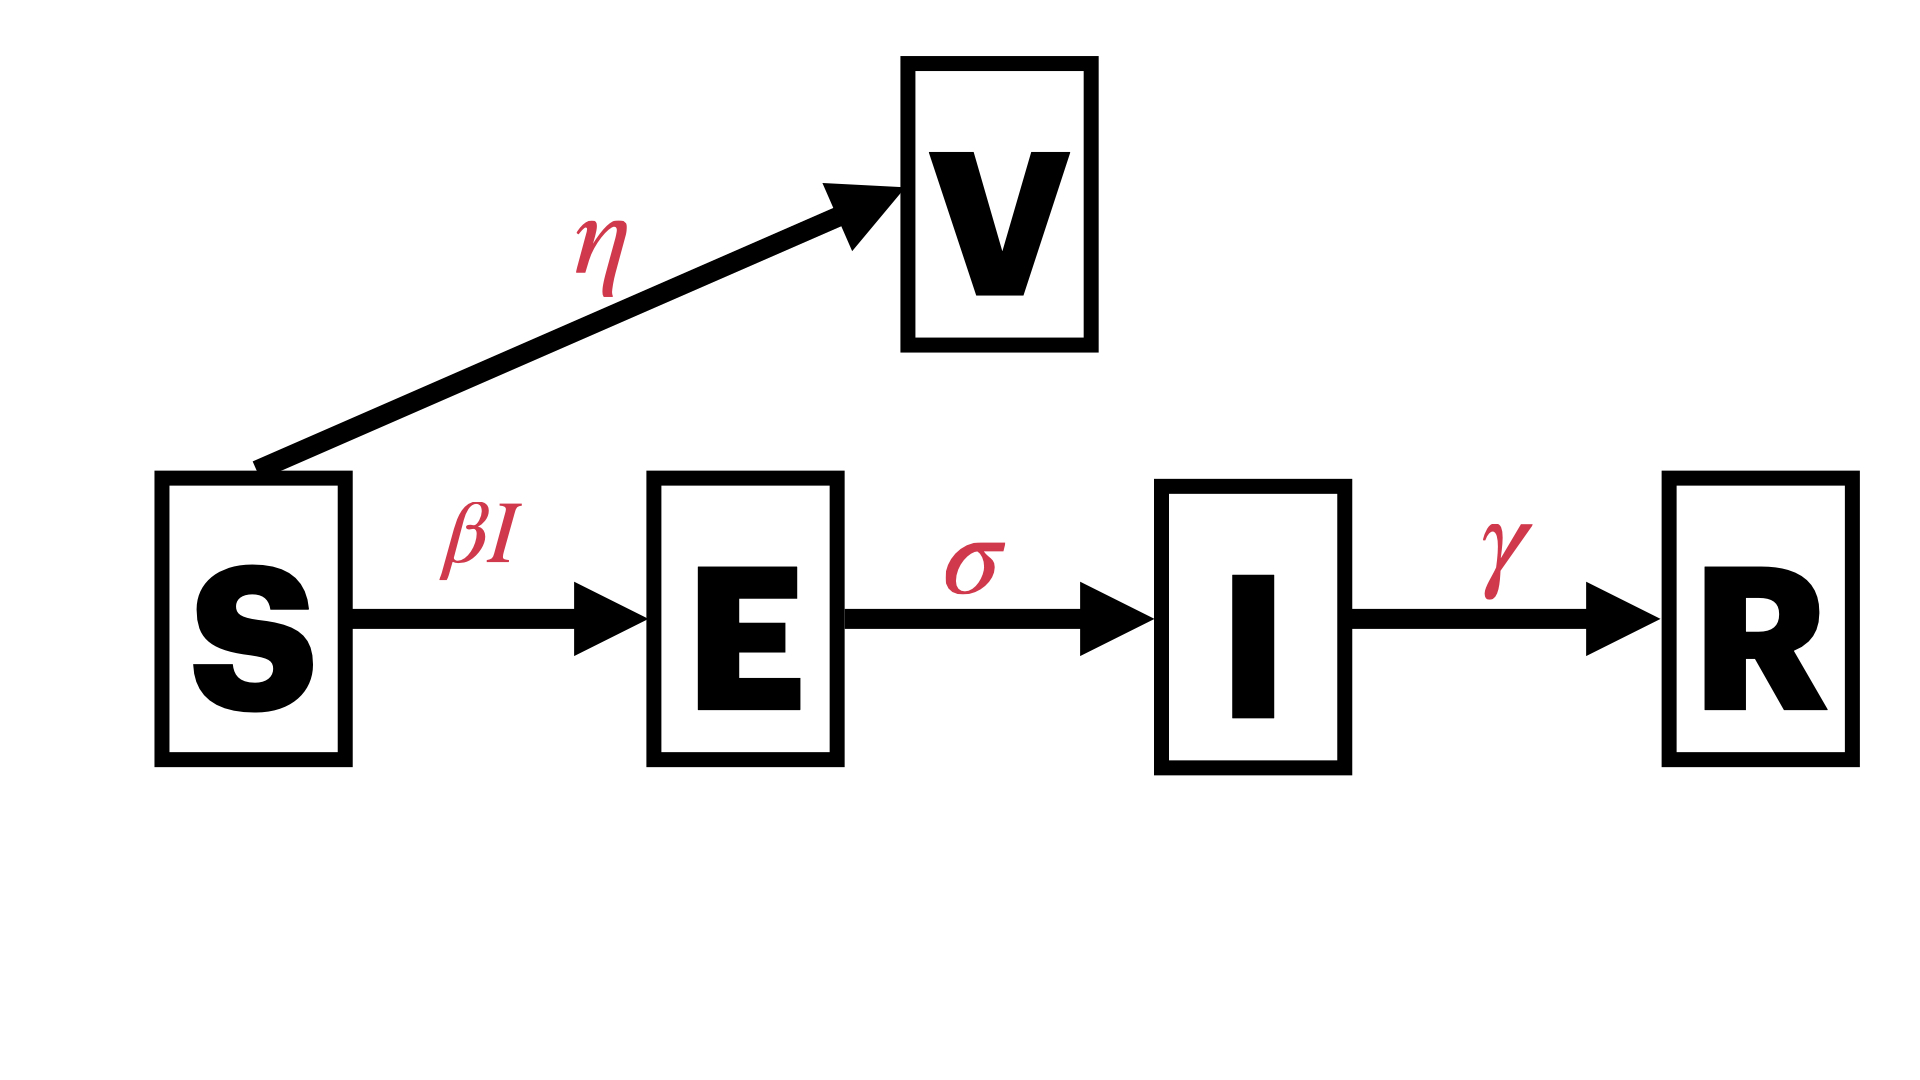
\includegraphics{images/model_diagrams/model_diagrams.010.jpeg}
\end{block}
\end{frame}

\begin{frame}
\begin{columns}[T]
\begin{column}{0.4\textwidth}
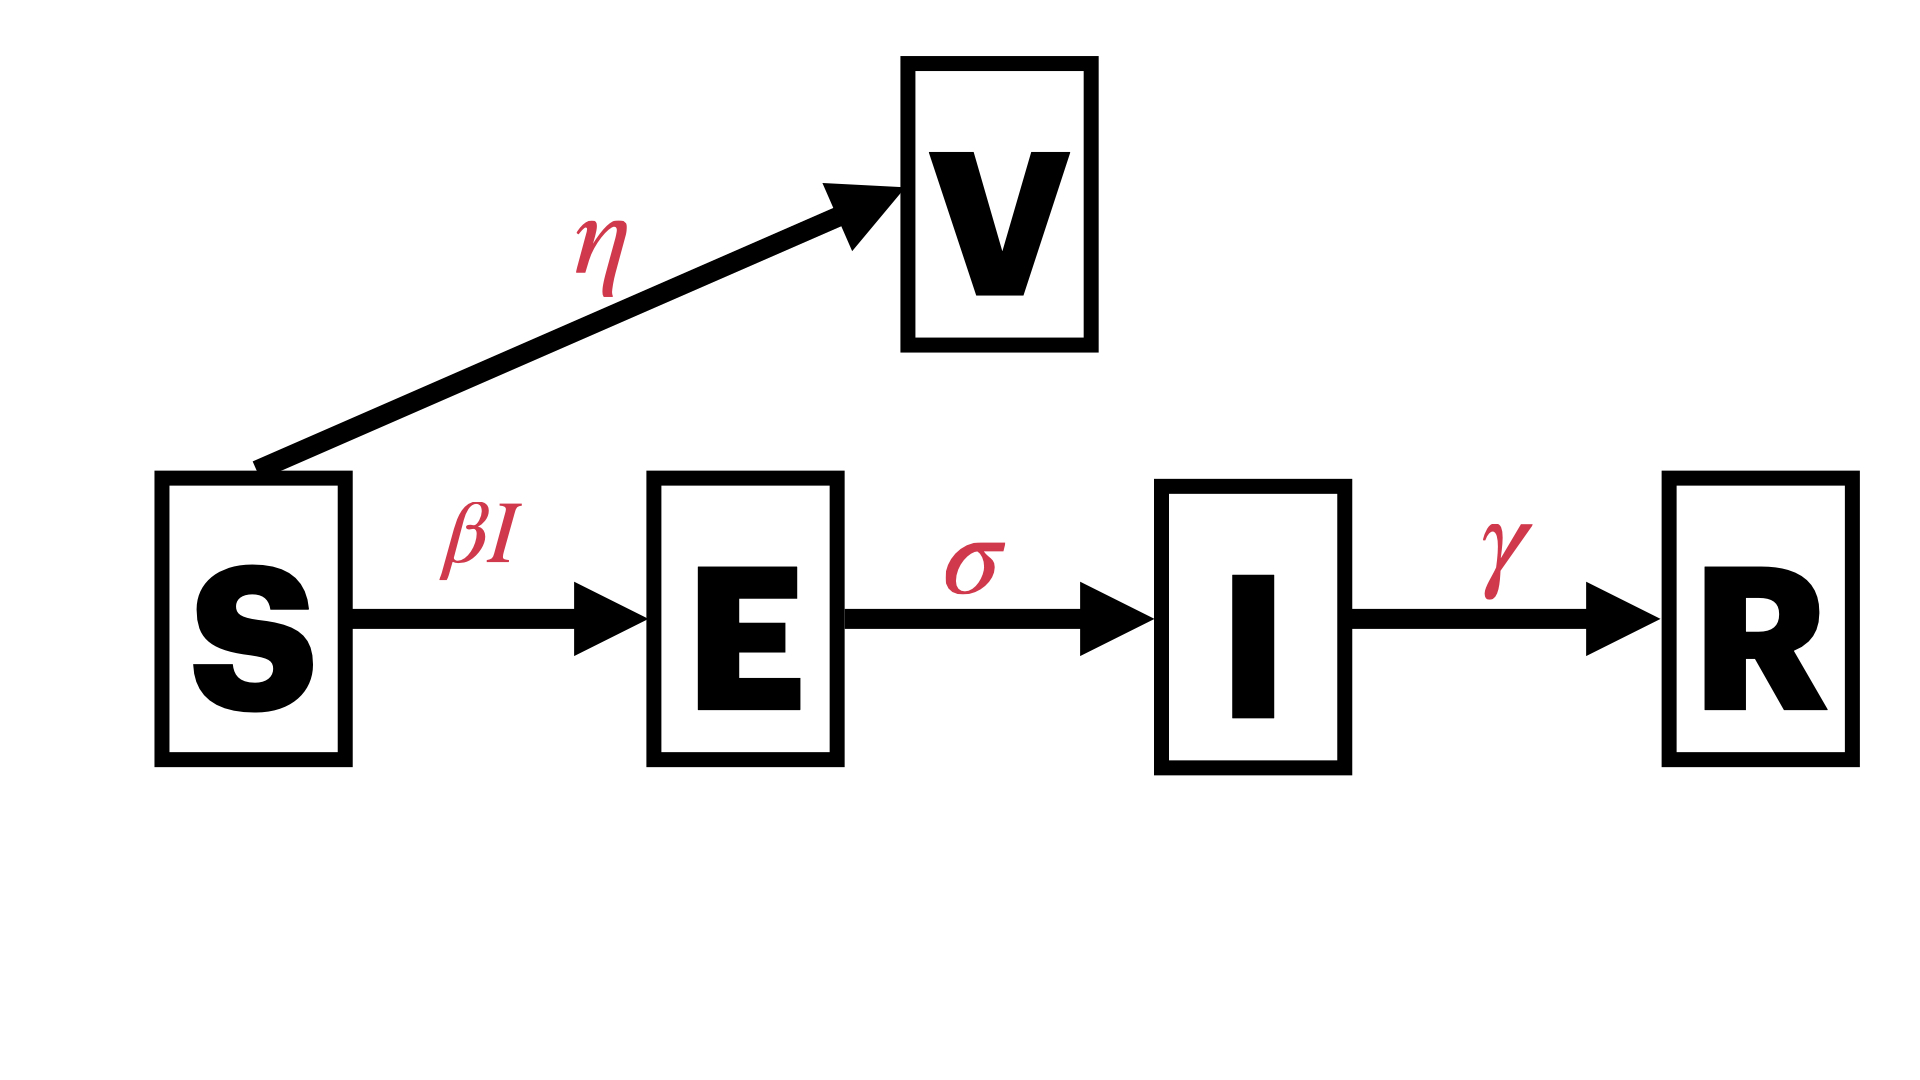
\includegraphics{images/model_diagrams/model_diagrams.010.jpeg}
\end{column}

\begin{column}{0.6\textwidth}
\begin{itemize}
\tightlist
\item
  The SEIRV model is simply the SEIR model with a vaccinated
  compartment, \(V\).
\item
  The vaccinated compartment represents previously susceptible
  individuals who have been vaccinated and are immune to the disease.
\end{itemize}
\end{column}
\end{columns}
\end{frame}

\begin{frame}
\begin{itemize}
\item
  The vaccinated compartment is:

  \begin{itemize}
  \item
    not infectious and does not move to the exposed or infectious
    compartments.
  \item
    replenished by the rate of vaccination, \(\eta\).
  \end{itemize}
\end{itemize}
\end{frame}

\begin{frame}
The model diagram and equations are as follows:

\begin{columns}[T]
\begin{column}{0.4\textwidth}
\begin{align}
\frac{dS}{dt} & = -\beta S I - \eta S \\
\frac{dE}{dt} & = \beta S I - \sigma E \\
\frac{dI}{dt} & = \sigma E - \gamma I \\
\frac{dR}{dt} & = \gamma I \\
\frac{dV}{dt} & = \eta S
\end{align}
\end{column}

\begin{column}{0.6\textwidth}
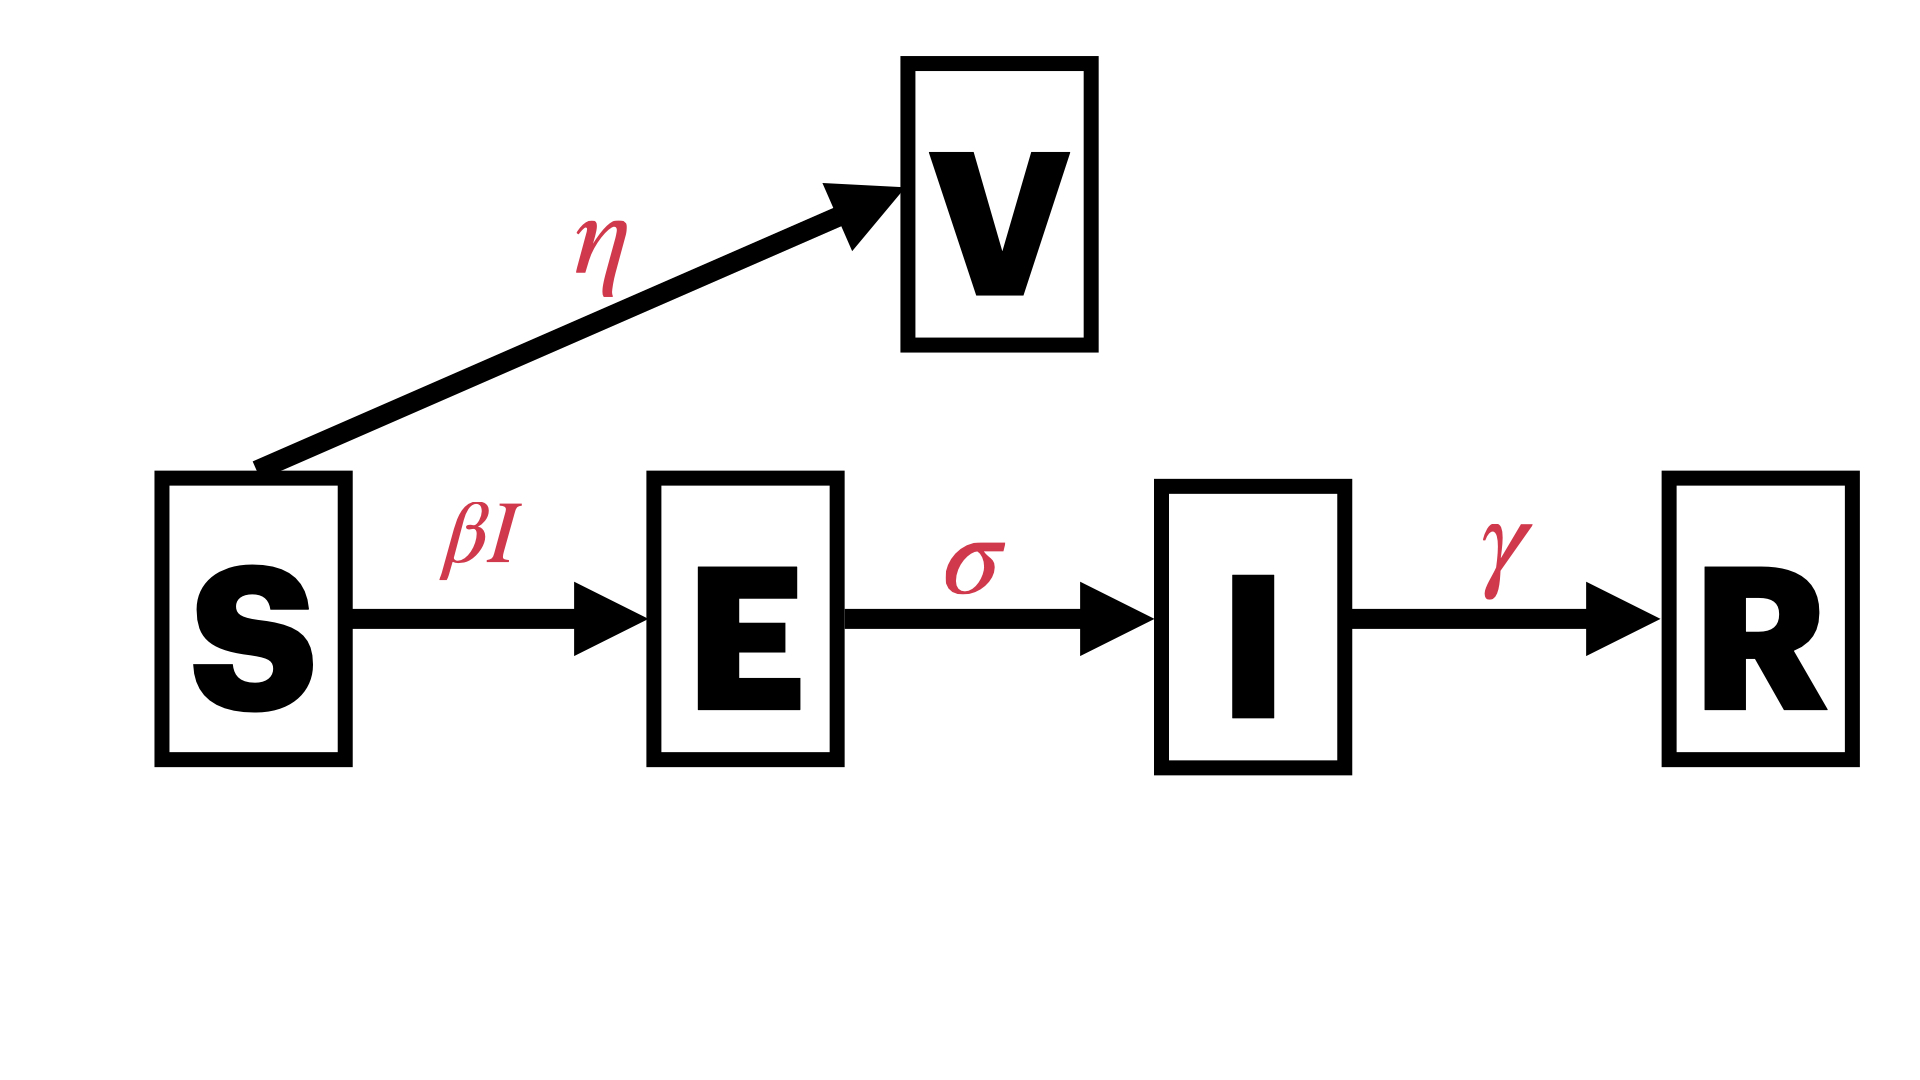
\includegraphics{images/model_diagrams/model_diagrams.010.jpeg}
\end{column}
\end{columns}

where \(\eta\) is the rate of vaccination.
\end{frame}

\begin{frame}
\begin{tcolorbox}[enhanced jigsaw, colframe=quarto-callout-caution-color-frame, toprule=.15mm, opacitybacktitle=0.6, breakable, colback=white, leftrule=.75mm, left=2mm, opacityback=0, titlerule=0mm, bottomtitle=1mm, toptitle=1mm, title={Discussion}, bottomrule=.15mm, arc=.35mm, coltitle=black, colbacktitle=quarto-callout-caution-color!10!white, rightrule=.15mm]

\begin{itemize}
\item
  What are some of the assumptions of the SEIRV model?
\item
  What are the implications of these assumptions for the model's
  predictions?
\end{itemize}

\end{tcolorbox}
\end{frame}

\begin{frame}[fragile]
\begin{block}{Numerical simulations}
\phantomsection\label{numerical-simulations-2}
\begin{block}{R Practicals}
\phantomsection\label{r-practicals-1}
\begin{itemize}
\item
  We can use the same approach as the SIR and SEIR models to simulate
  the SEIRV model.
\item
  Modify the \texttt{seir.Rmd} script to simulate the SEIRV model.
\end{itemize}
\end{block}
\end{block}
\end{frame}

\begin{frame}
\begin{block}{Non-Pharmaceutical Interventions (NPIs)}
\phantomsection\label{non-pharmaceutical-interventions-npis}
For a background on non-pharmaceutical interventions, refer to
Section~\ref{sec-npi}.
\end{block}
\end{frame}

\begin{frame}
\begin{itemize}
\item
  Conceptually, NPIs usually act to either reduce the transmission rate,
  \(\beta\) or prevent infected individuals from transmitting.
\item
  NPIs like isolation, social distancing and movement restrictions can
  reduce the transmission rate, \(\beta\), by reducing the contact rate
  between susceptible and infectious individuals.
\item
  Hygiene measures reduce the probability of transmission per contact,
  thereby reducing the transmission rate, \(\beta\), since
  \(\beta = c \times p\).
\end{itemize}
\end{frame}

\begin{frame}
\begin{itemize}
\item
  Let's consider two scenarios that will extend the SIR model to include
  NPIs:

  \begin{enumerate}
  \tightlist
  \item
    Modifying the transmission rate, \(\beta\).
  \item
    Preventing infected individuals from transmitting through isolation.
  \end{enumerate}
\end{itemize}
\end{frame}

\begin{frame}
\begin{block}{Modifying the transmission rate}
\phantomsection\label{modifying-the-transmission-rate}
\begin{itemize}
\item
  NPIs such as social distancing, mask-wearing, and hand hygiene can
  reduce the transmission rate, \(\beta\).
\item
  We can model this by making the transmission rate a function of time,
  \(\beta (t)\).
\end{itemize}
\end{block}
\end{frame}

\begin{frame}
The modified SIR model with a reduced transmission rate is as follows:

\begin{align*}
\frac{dS}{dt} & = -\beta (t) S I \\
\frac{dI}{dt} & = \beta (t) S I - \gamma I \\
\frac{dR}{dt} & = \gamma I
\end{align*}
\end{frame}

\begin{frame}
\begin{itemize}
\item
  The simplest form is to reduce \(\beta\) by an NPI efficacy, say
  \(\epsilon\).
\item
  Assuming the NPI is implemented between \(t_{\text{npi\_start}}\) and
  \(t_{\text{npi\_end}}\), it means that \(\beta\) remains the same
  before that period and is modified to \((1- \epsilon)\beta\) during
  the period of the NPI, where \(0 \leq \epsilon \leq 1\).
\item
  With this knowledge, we can define \(\beta (t)\) mathematically as:
\end{itemize}

\begin{equation*}
\beta(t) = \begin{cases}
\beta & \text{if } t < t_{\text{npi\_start}} \text{ or } t > t_{\text{npi\_end}} \\
(1 - \epsilon) \beta & \text{if } t_{\text{npi\_start}} \le t \le t_{\text{npi\_end}}
\end{cases}
\end{equation*}
\end{frame}

\begin{frame}[fragile]
\begin{block}{R Practicals}
\phantomsection\label{r-practicals-2}
\begin{itemize}
\tightlist
\item
  Let's open the script file \texttt{sir\_npi.R} and follow along.
\end{itemize}
\end{block}
\end{frame}

\begin{frame}
\begin{block}{NPIs as compartments}
\phantomsection\label{npis-as-compartments}
\begin{itemize}
\item
  In the previous example, we retained the SIR model structure and
  modified the transmission rate.
\item
  We can also model NPIs as compartments in the model. This is useful
  when we want to treat individuals affected by the NPIs differently.
\end{itemize}
\end{block}
\end{frame}

\begin{frame}
\begin{itemize}
\item
  For example, isolation is an NPI that prevents infected individuals
  from transmitting the disease.
\item
  This means that infected individuals in isolation do not contribute to
  the transmission of the disease and need to be removed from the
  infected compartment.
\item
  Moving isolated individuals to a separate compartment allows us to
  track them separately in the model and apply relevant parameters.
\end{itemize}
\end{frame}

\begin{frame}
\begin{itemize}
\item
  We can model this by introducing a new compartment, \(Q\), for
  isolating infected individuals.
\item
  Let's assume, infected individuals move to the isolated compartment at
  a rate, \(\delta\).
\item
  Infected individuals in the isolated compartment do not transmit the
  disease.
\end{itemize}
\end{frame}

\begin{frame}
The modified SIR model with isolated is as follows:

\begin{align*}
\frac{dS}{dt} & = -\beta S I \\
\frac{dI}{dt} & = \beta S I - \gamma I - \delta I \\
\frac{dR}{dt} & = \gamma I + \tau Q \\
\frac{dQ}{dt} & = \delta I - \tau Q
\end{align*}

where \(\delta\) is the rate at which infected individuals move to the
isolated compartment, and \(\tau\) is the rate at which individuals
recover from isolation.
\end{frame}

\begin{frame}[fragile]
\begin{block}{R Practicals}
\phantomsection\label{r-practicals-3}
\begin{itemize}
\tightlist
\item
  We can use the same approach as the SIR model to simulate the model
  with isolation.
\item
  Modify the SIR model in \texttt{sir.Rmd} to incorporate the isolated
  compartment, \(Q\) and the relevant parameters.
\end{itemize}
\end{block}
\end{frame}

\begin{frame}{Brief notes on modelling host heterogeneity}
\phantomsection\label{brief-notes-on-modelling-host-heterogeneity}
\begin{itemize}
\item
  The models we have discussed so far assume that all individuals in the
  population are identical.
\item
  However, in reality, individuals differ in their susceptibility to
  infection and their ability to transmit the disease.
\item
  It is essential to capture this heterogeneity in the models in order
  for the models to be more realistic and useful for decision-making.
\end{itemize}
\end{frame}

\begin{frame}
\begin{itemize}
\item
  This can be captured by incorporating heterogeneity into the models.
\item
  Heterogeneity is often captured by stratifying the population into
  different groups.
\end{itemize}
\end{frame}

\begin{frame}
\begin{block}{Age structure}
\phantomsection\label{age-structure}
\begin{itemize}
\item
  For many infectious diseases, the risk of infection and the severity
  of the disease vary by age.
\item
  Hence, it is essential to capture age structure in the models.
\item
  To do this, we divide the population into different age groups and
  model the disease dynamics within each age group.
\item
  Let's extend the SIR model to include age structure.
\end{itemize}
\end{block}
\end{frame}

\begin{frame}
\begin{itemize}
\item
  We will divide the population into \(n\) age groups.
\item
  Because the homogeneous model has 3 compartments, the age structured
  one will have \(3n\) compartments:
  \(S_1, I_1, R_1, S_2, I_2, R_2, ..., S_n, I_n, R_n\).
\end{itemize}
\end{frame}

\begin{frame}
\begin{itemize}
\tightlist
\item
  The (compact) model equations are as follows:
\end{itemize}

\begin{align*}
\dfrac{dS_i}{dt} &= -\sum_{j=1}^{n} \beta_{ji} S_i I_j \\
\dfrac{dI_i}{dt} &= \sum_{j=1}^{n} \beta_{ji} S_i I_j - \gamma I_i \\
\dfrac{dR_i}{dt} &= \gamma I_i
\end{align*}
\end{frame}

\begin{frame}
\begin{itemize}
\item
  The model can be used to study the impact of age structure on the
  dynamics of the epidemic.
\item
  For example, we can study the impact of vaccinating different age
  groups on the dynamics of the epidemic.
\end{itemize}
\end{frame}

\begin{frame}
\begin{block}{Other Heterogeneities}
\phantomsection\label{other-heterogeneities}
\begin{itemize}
\tightlist
\item
  Other forms of heterogeneity that can be incorporated into the models
  include:

  \begin{itemize}
  \tightlist
  \item
    Spatial heterogeneity
  \item
    Temporal heterogeneity
  \item
    Contact heterogeneity
  \item
    Heterogeneity in host behavior
  \end{itemize}
\end{itemize}
\end{block}
\end{frame}

\begin{frame}{Final Remarks}
\phantomsection\label{final-remarks}
\begin{block}{Takeaways}
\phantomsection\label{takeaways}
In the last two days, we have covered a lot of ground. Here are some key
takeaways:

\begin{itemize}
\item
  Infectious diseases are a major public health concern that can have
  devastating consequences.
\item
  Mathematical models are essential tools for studying the dynamics of
  infectious diseases and informing public health decision-making.
\item
  Models are simplifications of reality that help us understand complex
  systems.
\end{itemize}
\end{block}
\end{frame}

\begin{frame}
\begin{itemize}
\item
  We have discussed several compartmental models, including the SIR,
  SEIR, and SEIRV models.
\item
  The SIR model is a simple compartmental model that divides the
  population into three compartments: susceptible, infected, and
  recovered.
\item
  The SEIR model extends the SIR model by adding an exposed compartment.
\item
  We can model various pharmaceutical and non-pharmaceutical
  interventions (NPIs) by modifying the transmission rate or adding new
  compartments.
\end{itemize}
\end{frame}

\begin{frame}
\begin{itemize}
\item
  We have discussed the basic reproduction number, \(R0\), which is a
  key parameter in infectious disease epidemiology.
\item
  \(R0\) is the average number of secondary infections produced by a
  single infected individual in a completely susceptible population.
\item
  If \(R0 > 1\), the disease will spread in the population; if
  \(R0 < 1\), the disease will die out.
\end{itemize}
\end{frame}

\begin{frame}
\begin{itemize}
\item
  Deriving the basic reproduction number, \(R0\), is an essential step
  in understanding the dynamics of infectious diseases.
\item
  Deriving \(R0\) for the simple SIR model is simple as we just need to
  study the threshold phenomena.
\item
  For more complex models, we can use the next-generation matrix
  approach to derive \(R0\).
\end{itemize}
\end{frame}

\begin{frame}
\begin{itemize}
\item
  Often, homogeneous models are not sufficient to capture the complexity
  of infectious diseases.
\item
  Incorporating heterogeneity into the models is essential for capturing
  the complexity of infectious diseases.
\item
  Age structure is a common form of heterogeneity that can be
  incorporated into the models.
\item
  Other forms of heterogeneity include spatial, temporal, and contact
  heterogeneity.
\end{itemize}
\end{frame}

\begin{frame}
\begin{block}{What skills are needed to build and use infectious disease
models?}
\phantomsection\label{what-skills-are-needed-to-build-and-use-infectious-disease-models}
\begin{figure}[H]

{\centering 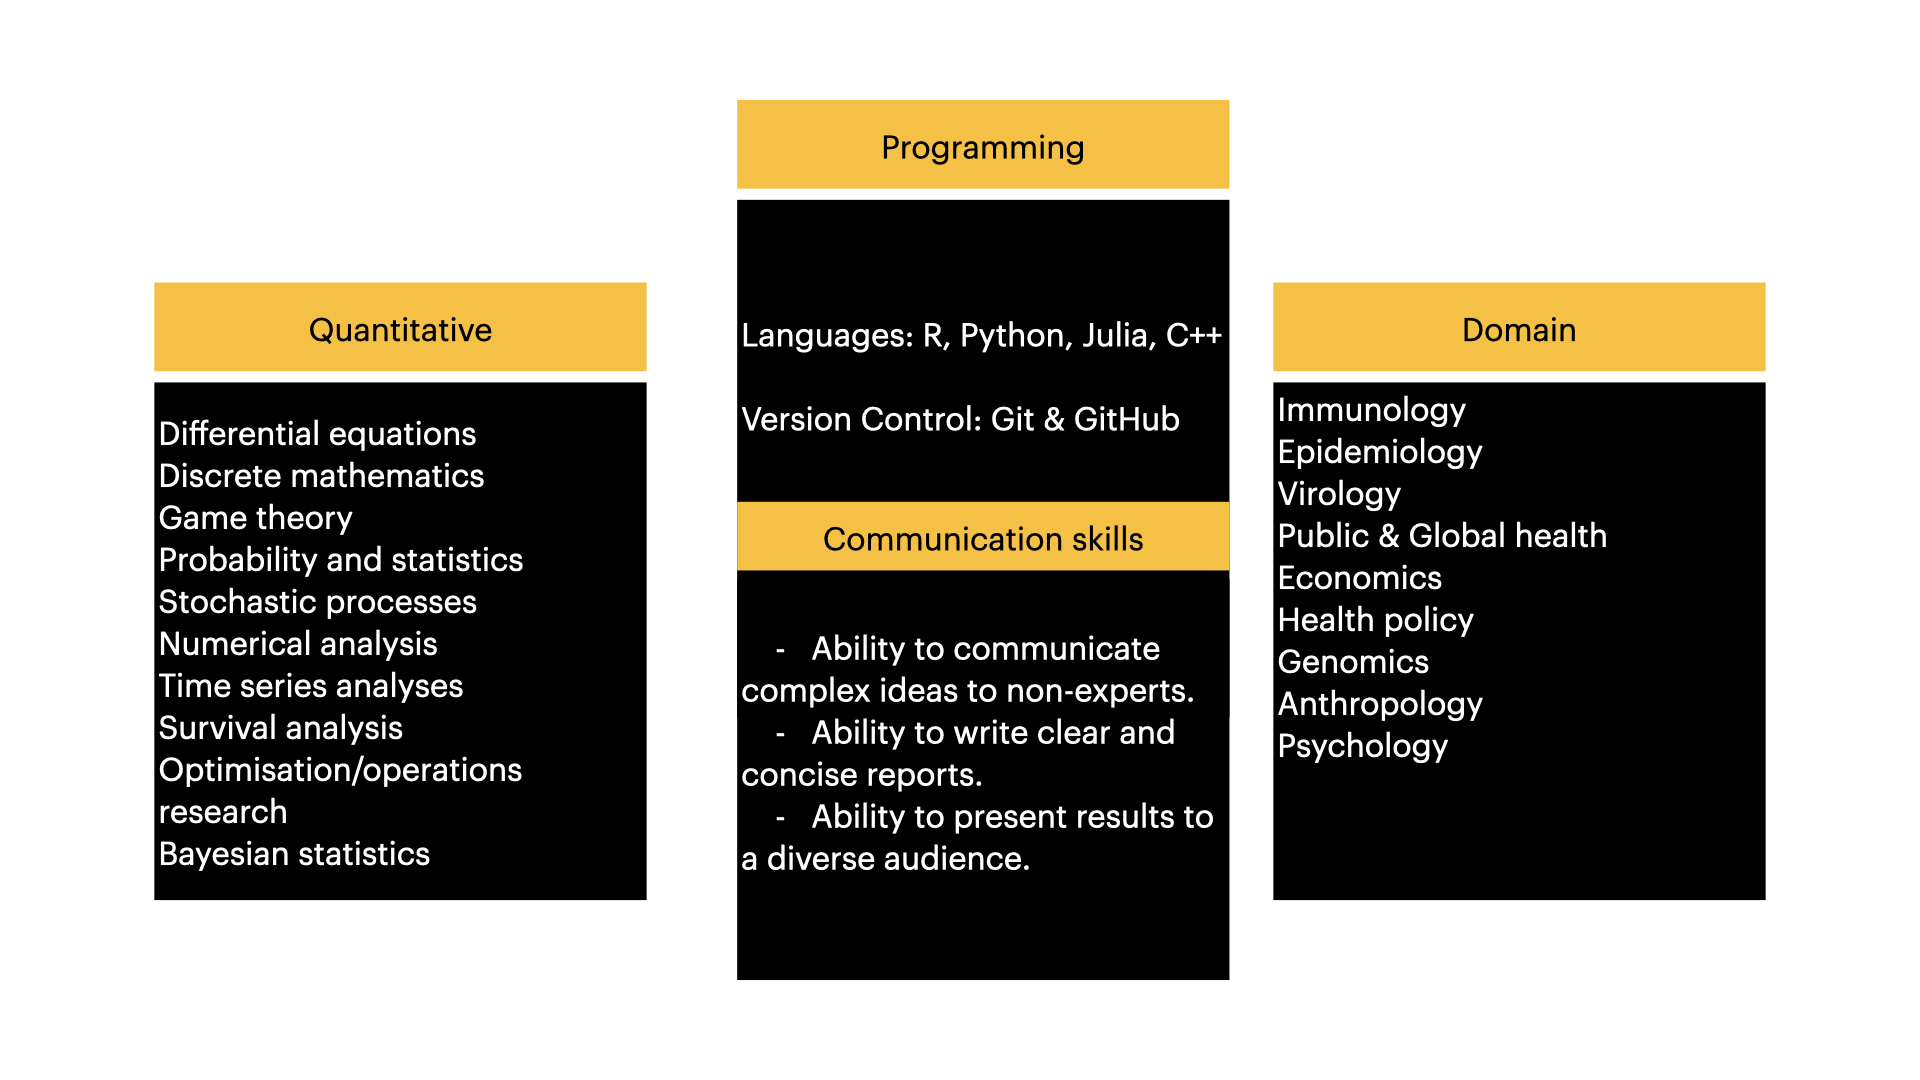
\includegraphics{images/modelling_skills.jpeg}

}

\caption{A non-exhaustive list of skills needed for modelling infectious
diseases.}

\end{figure}%
\end{block}
\end{frame}

\begin{frame}
\begin{block}{Contact Information}
\phantomsection\label{contact-information}
\textbf{James Mba Azam, PhD}

\href{https://epiverse-trace.github.io/}{\emph{Epiverse-TRACE
Initiative, London School of Hygiene and Tropical Medicine, UK}}

\textbf{Email:}
\href{mailto:james.azam@lshtm.ac.uk}{\nolinkurl{james.azam@lshtm.ac.uk}}

\textbf{ORCID:}
\href{https://orcid.org/0000-0001-5782-7330}{0000-0001-5782-7330}

\textbf{Social Media:}

\textbf{LinkedIn:}
\href{https://www.linkedin.com/in/james-azam-phd-6b5b00176/}{James Azam}

\textbf{Twitter:} \href{https://twitter.com/james_azam}{james\_azam}

\textbf{GitHub:} \href{https://github.com/jamesmbaazam}{jamesmbaazam}
\end{block}
\end{frame}

\begin{frame}

\includegraphics{slides_files/mediabag/88x31.png} This presentation is
made available through a
\href{https://creativecommons.org/licenses/by/4.0/}{Creative Commons
Attribution 4.0 International License}
\end{frame}

\begin{frame}{List of Resources}
\phantomsection\label{list-of-resources}
\begin{block}{Textbooks}
\phantomsection\label{textbooks}
\begin{figure}

\begin{minipage}{0.50\linewidth}

\begin{figure}[H]

{\centering 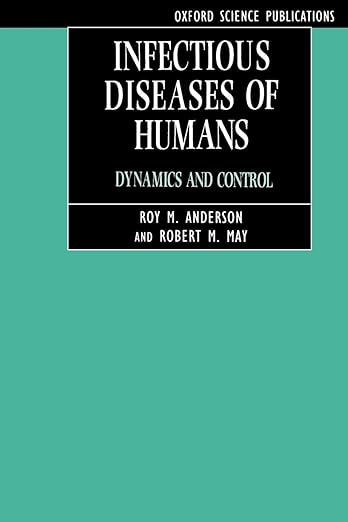
\includegraphics[width=0.6\textwidth,height=\textheight]{images/Anderson_and_May.jpeg}

}

\subcaption{Infectious Diseases of Humans: Dynamics and Control by Roy
M. Anderson and Robert M. May}

\end{figure}%

\end{minipage}%
%
\begin{minipage}{0.50\linewidth}

\begin{figure}[H]

{\centering 
\includegraphics[width=0.6\textwidth,height=\textheight]{images/ID_modelling_Vynnycky_and_White.jpeg}

}

\subcaption{Infectious Disease Modelling by Emilia Vynnycky and Richard
White}

\end{figure}%

\end{minipage}%

\end{figure}%
\end{block}
\end{frame}

\begin{frame}
\begin{figure}

\begin{minipage}{0.50\linewidth}

\begin{figure}[H]

{\centering 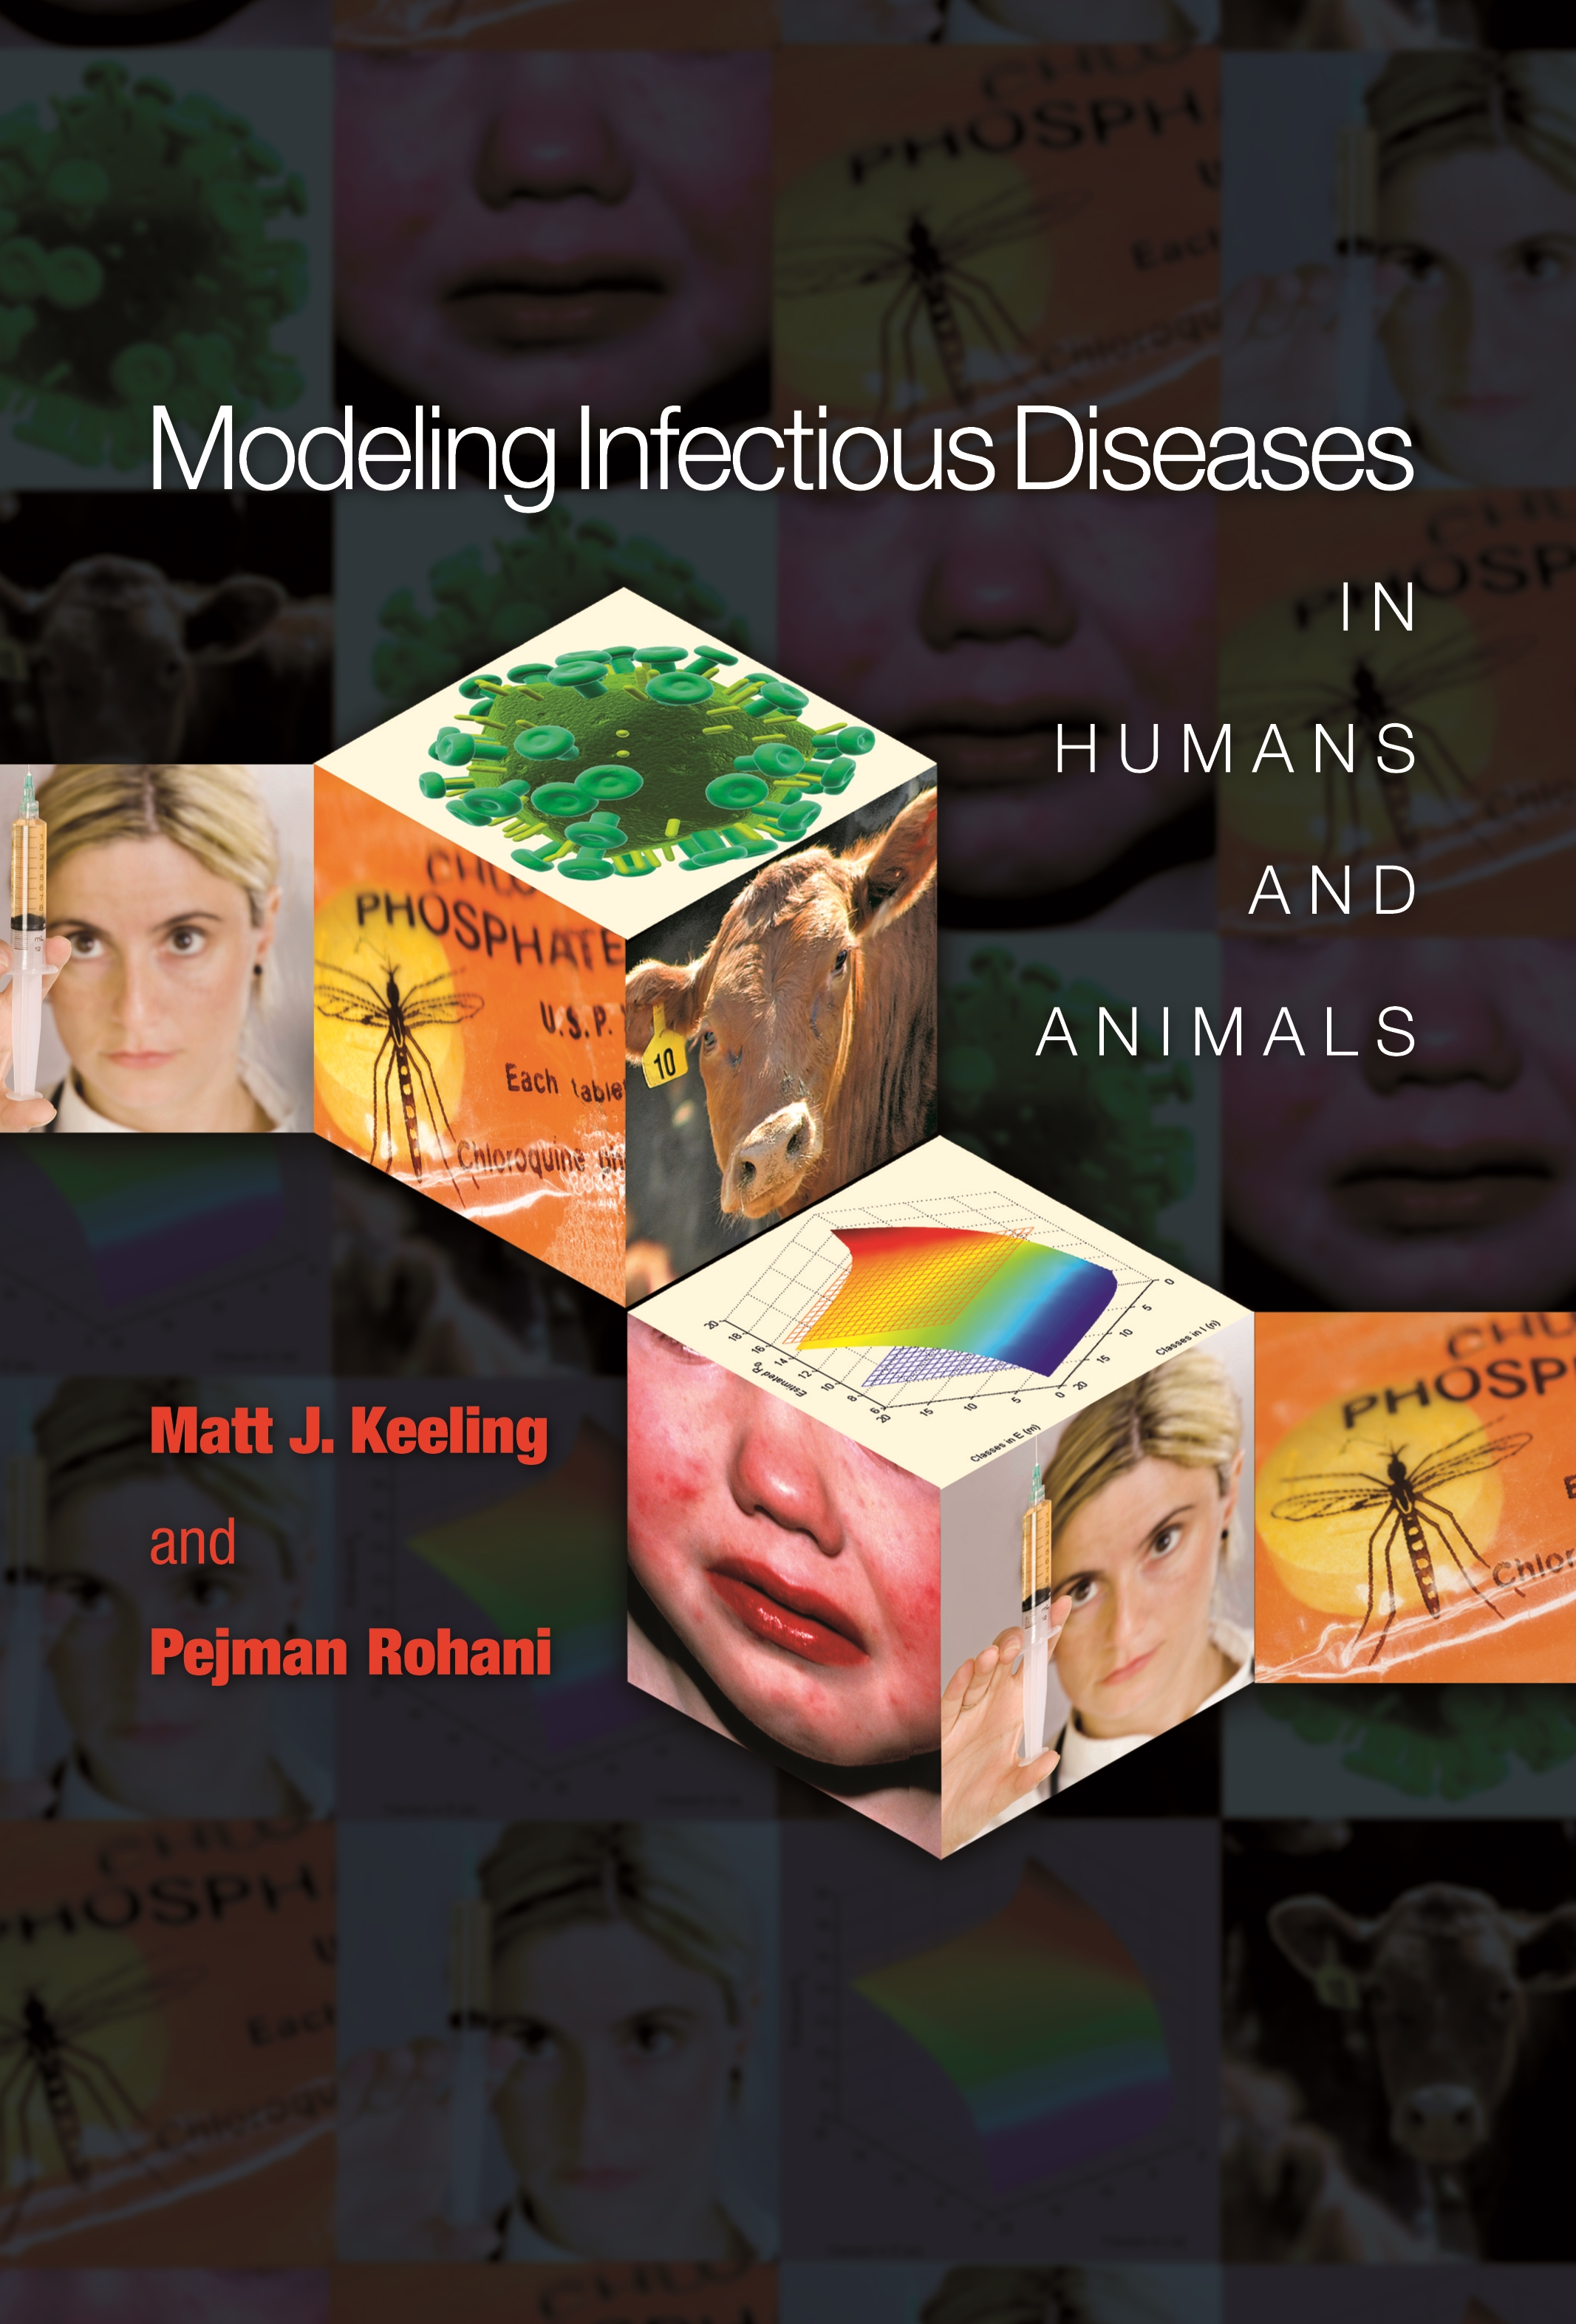
\includegraphics[width=0.6\textwidth,height=\textheight]{images/Rohani_and_Keeling.jpeg}

}

\subcaption{Modeling Infectious Diseases in Humans and Animals by Matt
Keeling and Pejman Rohani}

\end{figure}%

\end{minipage}%
%
\begin{minipage}{0.50\linewidth}

\begin{figure}[H]

{\centering 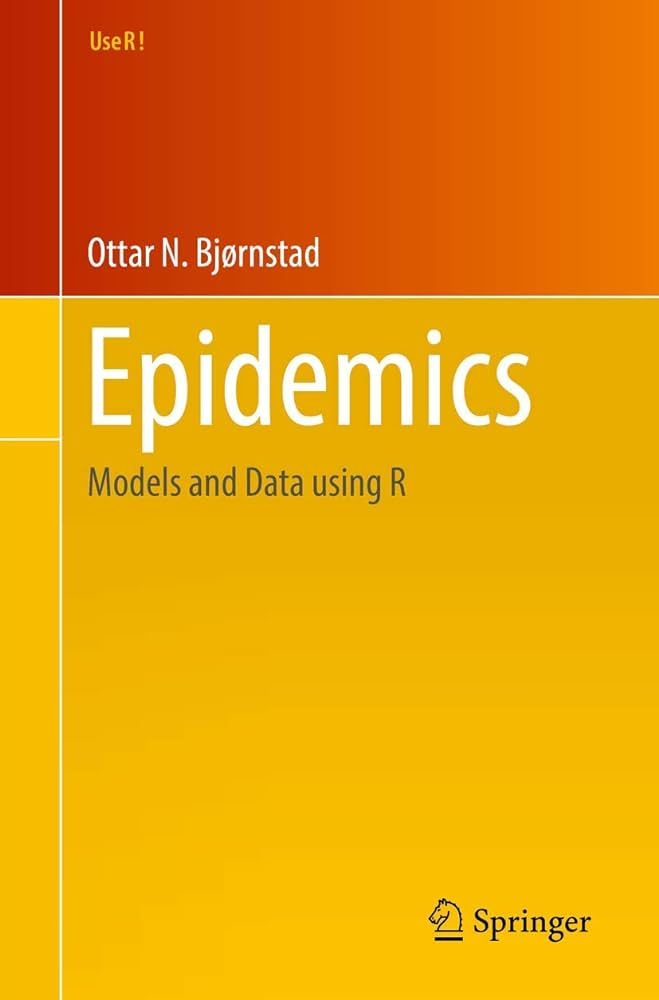
\includegraphics[width=0.6\textwidth,height=\textheight]{images/Epidemics_Ottar.jpg}

}

\subcaption{Epidemics: Models and Data Using R by Ottar N. Bjornstad}

\end{figure}%

\end{minipage}%

\end{figure}%
\end{frame}

\begin{frame}
\begin{block}{Papers and Articles}
\phantomsection\label{papers-and-articles}
\end{block}
\end{frame}

\begin{frame}
\begin{block}{Modelling infectious disease transmission}
\phantomsection\label{modelling-infectious-disease-transmission}
\begin{itemize}
\item
  Grassly, N. C., \& Fraser, C. (2008). Mathematical models of
  infectious disease transmission. Nature Reviews Microbiology, 6(6),
  477--487. \url{https://doi.org/10.1038/nrmicro1845}
\item
  Kirkeby, C., Brookes, V. J., Ward, M. P., Dürr, S., \& Halasa, T.
  (2021). A practical introduction to mechanistic modeling of disease
  transmission in veterinary science. Frontiers in veterinary science,
  7, 546651.
  \url{https://www.frontiersin.org/articles/10.3389/fvets.2020.546651/full}
\end{itemize}
\end{block}
\end{frame}

\begin{frame}
\begin{itemize}
\tightlist
\item
  Blackwood, J. C., \& Childs, L. M. (2018). An introduction to
  compartmental modeling for the budding infectious disease modeler.
  \url{https://vtechworks.lib.vt.edu/items/61e9ca00-ef21-4356-bcd7-a9294a1d2f17}
\end{itemize}
\end{frame}

\begin{frame}
\begin{itemize}
\item
  Cobey, S. (2020). Modeling infectious disease dynamics. Science,
  368(6492), 713--714. \url{https://doi.org/10.1126/science.abb5659}
\item
  Bjørnstad, O. N., Shea, K., Krzywinski, M., \& Altman, N. (2020).
  Modeling infectious epidemics. Nature Methods, 17(5), 455--456.
  \url{https://doi.org/10.1038/s41592-020-0822-z}
\end{itemize}
\end{frame}

\begin{frame}
\begin{itemize}
\item
  Bodner, K., Brimacombe, C., Chenery, E. S., Greiner, A., McLeod, A.
  M., Penk, S. R., \& Soto, J. S. V. (2021). Ten simple rules for
  tackling your first mathematical models: A guide for graduate students
  by graduate students. PLOS Computational Biology, 17(1), e1008539.
  \url{https://doi.org/10.1371/journal.pcbi.1008539}
\item
  Mishra, S., Fisman, D. N., \& Boily, M.-C. (2011). The ABC of terms
  used in mathematical models of infectious diseases. Journal of
  Epidemiology \& Community Health, 65(1), 87--94.
  \url{https://jech.bmj.com/content/65/1/87}
\end{itemize}
\end{frame}

\begin{frame}
\begin{itemize}
\item
  James, L. P., Salomon, J. A., Buckee, C. O., \& Menzies, N. A. (2021).
  The Use and Misuse of Mathematical Modeling for Infectious Disease
  Policymaking: Lessons for the COVID-19 Pandemic. 41(4), 379--385.
  \url{https://doi.org/10.1177/0272989X21990391}
\item
  Holmdah, I., \& Buckee, C. (2020). Wrong but useful---What COVID-19
  epidemiologic models can and cannot tell us. New England Journal of
  Medicine. \url{https://doi.org/10.1056/nejmp2009027}
\end{itemize}
\end{frame}

\begin{frame}
\begin{itemize}
\item
  Metcalf, C. J. E. E., Edmunds, W. J., \& Lessler, J. (2015). Six
  challenges in modelling for public health policy. Epidemics, 10(2015),
  93--96. \url{https://doi.org/10.1016/j.epidem.2014.08.008}
\item
  Roberts, M., Andreasen, V., Lloyd, A., \& Pellis, L. (2015). Nine
  challenges for deterministic epidemic models. Epidemics, 10(2015),
  49--53. \url{https://doi.org/10.1016/j.epidem.2014.09.006}
\end{itemize}
\end{frame}

\begin{frame}
\begin{block}{Deriving and Interpreting R0}
\phantomsection\label{deriving-and-interpreting-r0}
\begin{itemize}
\item
  Jones, J. H. (2011). Notes On R0. Building, 1--19.
  \url{https://web.stanford.edu//~jhj1/teachingdocs/Jones-on-R0.pdf}
\item
  Diekmann, O., Heesterbeek, J. A. P., \& Metz, J. A. J. (1990). On the
  definition and the computation of the basic reproduction ratio R0 in
  models for infectious diseases in heterogeneous populations. Journal
  of Mathematical Biology, 28(4), 365--382.
  \url{https://doi.org/10.1007/BF00178324}
\end{itemize}
\end{block}
\end{frame}

\begin{frame}
\begin{itemize}
\tightlist
\item
  Diekmann, O., Heesterbeek, J. A. P., \& Roberts, M. G. (2010). The
  construction of next-generation matrices for compartmental epidemic
  models. Journal of the Royal Society Interface, 7(47), 873--885.
  \url{https://doi.org/10.1098/rsif.2009.0386}
\end{itemize}
\end{frame}

\begin{frame}
\begin{block}{Code repositories}
\phantomsection\label{code-repositories}
\begin{itemize}
\item
  \href{http://epirecip.es/epicookbook/}{epirecipes}: Code for collate
  mathematical models of infectious disease transmission, with
  implementations in R, Python, and Julia.
\item
  \href{http://www.modelinginfectiousdiseases.org/}{Modeling Infectious
  Diseases in Humans and Animals}: Code for the labelled programs in the
  book ``Modeling Infectious Diseases in Humans and Animals''. They are
  generally available as C++, Fortran and Matlab files.
\end{itemize}
\end{block}
\end{frame}

\begin{frame}{References}
\phantomsection\label{references}
\phantomsection\label{refs}
\begin{CSLReferences}{1}{0}
\bibitem[\citeproctext]{ref-Blackwood2018a}
Blackwood, Julie C., and Lauren M. Childs. 2018. {``An Introduction to
Compartmental Modeling for the Budding Infectious Disease Modeler.''}
\emph{Letters in Biomathematics} 5 (1): 195--221.
\url{https://doi.org/10.1080/23737867.2018.1509026}.

\bibitem[\citeproctext]{ref-Box1979}
Box, GE. 1979. {``All Models Are Wrong, but Some Are Useful.''}
\emph{Robustness in Statistics} 202 (1979): 549.

\bibitem[\citeproctext]{ref-kermack1927contribution}
Kermack, William Ogilvy, and Anderson G McKendrick. 1927. {``A
Contribution to the Mathematical Theory of Epidemics.''}
\emph{Proceedings of the Royal Society of London. Series A, Containing
Papers of a Mathematical and Physical Character} 115 (772): 700--721.

\end{CSLReferences}
\end{frame}



\end{document}
